\documentclass[a4paper,landscape,twocolumn]{article}
\usepackage[utf8]{inputenc}
\usepackage[T1]{fontenc}
\usepackage[ngerman,english]{babel}
\usepackage{amsmath}
\usepackage{amssymb}
\usepackage{amsthm}
\usepackage{csquotes}
\usepackage{fancyhdr}
\usepackage[margin=1in]{geometry}
\usepackage[makeindex]{imakeidx}  % before hyperref
\usepackage[pdfborder={0 0 0}]{hyperref}
\usepackage{marvosym}
\usepackage{mathtools}
\usepackage{mdframed}
\usepackage{stmaryrd}
\usepackage[normalem]{ulem}
\usepackage{wasysym}

\parskip5pt
\parindent0pt

\theoremstyle{definition}

\newtheorem{theorem}{Theorem}
\newtheorem{defi}{Definition}
\newtheorem{rem}{Remark}
\newtheorem{ex}{Example}
\newtheorem{cor}{Corollary}
\newtheorem{lemma}{Lemma}

\newcommand\okay{\qquad\checkmark}
\newcommand\set[1]{\left\{#1\right\}}
\newcommand\setdef[2]{\left\{#1\,\middle|\,#2\right\}}
\newcommand\abs[1]{\left|#1\right|}
\newcommand\seq[1]{{\left(#1\right)}_{n \in \mathbb N}}
\newcommand\reg{\mathcal B}
\newcommand\card[1]{\left|\,#1\,\right|}
\newcommand\meta[3]{\hrule{} This #1 took place on #2 with lecturer #3.\par}
\newcommand\done{\hspace{10pt}\checkmark}
\newcommand\norm[1]{\left\|#1\right\|}
\newcommand\inorm[1]{\left\|#1\right\|_\infty}
\newcommand\fun[1]{\left\langle{#1}\right\rangle}

\pagestyle{fancy}
\fancyhf{}
\chead{\Large{\textsc{Mathematical Analysis II -- Lecture Notes}}}
\lfoot{\makebox[\columnwidth]{\thepage}}
\rfoot{\makebox[\columnwidth]{\number\numexpr\value{page}+1}\stepcounter{page}}
\setlength{\headheight}{18pt}

\makeindex[name={German},title={German keywords}]
\makeindex[name={English},title={English keywords}]
\twocolumn

\title{
  Mathematical analysis 2 -- Lecture notes \\
  \small{course by Wolfgang Ring}
}
\author{Lukas Prokop}
\date{March to July 2016}

\begin{document}
\maketitle
\tableofcontents

\clearpage
\meta{lecture}{1st of March 2016}{Wolfgang Ring}

Course organization:
\begin{itemize}
  \item Tuesday, 1 hours 30 minutes, beginning at 8:15
  \item Thursday, 45 minutes, beginning at 8:15
  \item Friday, 1 hours 30 minutes, beginning at 8:15
\end{itemize}

Literature:
\begin{itemize}
  \item Königsberger, Analysis 1
\end{itemize}

\clearpage
\section{Exponential function (cont.)}
%
Let $(z_n)_{n \in \mathbb N}$ be a complex series with $\lim_{n\to\infty} z_n = z$
and $\lim_{n\to\infty} (1 + \frac{z_n}{n})^n = \sum_{k=0}^\infty \frac{z^k}{k!}$.
For every complex number $z \in \mathbb C$ this series converges on entire $\mathbb C$.

\[ \exp(z) = \lim_{n\to\infty} \left(1 + \frac{z}n\right)^n = \sum_{k=0}^\infty \frac{z^k}{k!} \]
\[ \exp(z + w) = \exp(z) \cdot \exp(w) \]
\[ \lim_{z\to0} \frac{\exp(z) - 1}{z} = 1 \]
\[ \exp(1) = e \in \mathbb R \]
\[ z = \frac mn \in \mathbb Q \land n \neq 0 \Rightarrow \exp\left(\frac mn\right) = e^{\frac mn} \]

So we also denote
\[ \exp(z) = e^z \qquad \text{for } z \in \mathbb C \]
It holds that
\[ \exp(z) \neq 0 \qquad \forall z \in \mathbb C \]

$\exp(x)$ for $x \in \mathbb R$
\[ e^x > 0 \qquad \forall x \in \mathbb R \]

\[ (e^x)' = e^x \]
It follows immediately that the exponential function is strictly monotonically increasing in $\mathbb R$.
\[ (e^x)'' = (e^x)' = e^x > 0 \]
It follows that the exponential function is convex. But as usual,
\[ e^0 = 1 \]

\begin{figure}[!h]
  \begin{center}
    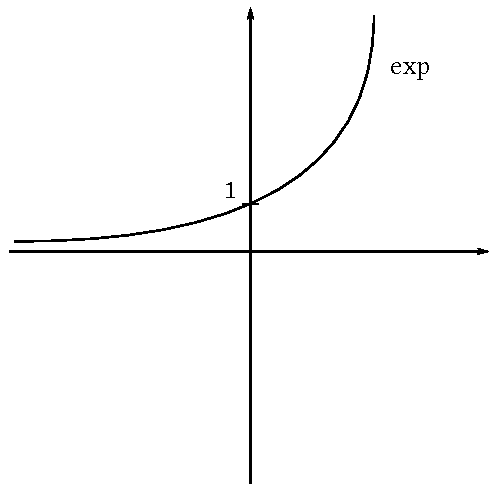
\includegraphics{img/exp-graph.pdf}
    \caption{Graph of the exponential function}
  \end{center}
\end{figure}

Let $n \in \mathbb N$
\[ \lim_{x\to+\infty} \frac{e^x}{x^n} = \infty \]
\[ \lim_{x\to-\infty} e^x \cdot x^n = 0 \]

\section{The natural logarithm}
%
\[ \exp: \mathbb R \to (0,\infty) \]
is injective, because $x_1 < x_2 \Rightarrow e^{x_1} < e^{x_2}$

\begin{lemma}
  $\exp: \mathbb R \to (0,\infty)$
  is surjective.
\end{lemma}
\begin{proof}
  We need to show that the equation $e^x = y$ has some solution for every $y > 0$.
  We will use the Intermediate Value Theorem, we discussed in the previous course \enquote{Analysis 1}.

  \begin{description}
    \item[Case 1]
      First of all, let $y \in [1,\infty)$. Then it holds that
      \[ e^0 = 1 \leq y \quad\text{and}\quad e^y = 1 + y + \underbrace{\frac{y^2}{2} + \frac{y^3}{3!} + \frac{y^4}{4!} + \ldots}_{\geq 0} \]
      \[ \geq 1 + y > y \]
      Therefore $e^0 \leq y < e^y$.
      Hence $\exp$ is continuous and the Intermediate Value Theorem applies:
      \[ \exists \xi \in [0,y]: \quad e^\xi = y \]
    \item[Case 2]
      Let $y \in (0,1)$. Then it holds that $w = \frac1{y} > 1$.
      The same as in Case~1 applies:
      \[ \exists \xi \in [0,w]: \quad e^\xi = w = \frac1{y} \]
      \[ \Rightarrow e^{-\xi} = \frac{1}{e^\xi} = y \]
  \end{description}

  So it holds that $\exp: \mathbb R \to (0,\infty)$ is bijective.
\end{proof}

\index[English]{Natural logarithm}
\index[German]{\foreignlanguage{ngerman}{Natürlicher Logarithmus}}
\begin{defi}
  We call the inverse function \emph{natural logarithm}\footnote{In non-German literature $\ln(y)$ is almost exclusively written with the more general $\log(y)$.}.
  \[ \exp^{-1}: (0,\infty) \to \mathbb R \]
  \[ \exp^{-1} = \ln(y) = \log(y) \]

  Properties:
  \begin{itemize}
    \item It holds $\forall x \in \mathbb R: \ln(e^x) = x$ and $\forall y \in (0,\infty): e^{\ln(y)} = y$.
    \item $\ln: (0,\infty) \to \mathbb R$ is strictly monotonically increasing
      \begin{proof}
        Let $0 < y_1 < y_2$. Assume $\ln(y_1) \geq \ln(y_2) \xRightarrow{\text{monotonicity}} e^{\ln(y_1)} \geq e^{\ln(y_2)} \Rightarrow y_1 \geq y_2$. Contradiction!
      \end{proof}
  \end{itemize}
\end{defi}

\subsection{Functional equations of logarithm}
%
\begin{itemize}
  \item
    For all $x,y > 0$ it holds that
    \[ \ln(x \cdot y) = \ln(x) + \ln(y) \]
  \item Limes:
    \[ \lim_{x \to 1} \frac{\ln(x)}{x - 1} = 1 \]
\end{itemize}
\begin{proof}
  \begin{itemize}
    \item
      \[ x \cdot y = e^{\ln(x \cdot y)} \]
      \[ e^{\ln(x)} \cdot e^{\ln(y)} = e^{\ln(x) + \ln(y)} \]
      Injectivity of $\exp$:
      \[ \ln(x \cdot y) = \ln(x) + \ln(y) \]
    \item
      Let $(x_n)_{n\in\mathbb N}$ with $x_n > 0$ be an arbitrary
      sequence with $\lim_{n\to\infty} x_n = 0$.
      Let $w_n = 1 + x_n$. Then it holds that
      $\lim_{n\to\infty} w_n = 1$ and $y_n = \ln(1 + x_n) = \ln(w_n)$.
      \[ \lim_{n\to\infty} y_n = \ln(1) = 0 \]
      \[ \lim_{n\to\infty} \frac{\ln(w_n)}{w_n - 1} = \lim_{n\to\infty} \frac{y_n}{e^{y_n} - 1} = \frac11 = 1 \]
      where
      \[ e^0 = 1 \Rightarrow \ln(1) = 0 \]
  \end{itemize}
\end{proof}

\begin{theorem}[Logarithmic growth]
  $\forall n \in \mathbb N_+$ it holds that $\lim_{n\to\infty} \frac{\ln(x)}{\sqrt[n]{x}} = 0$
\end{theorem}
\begin{proof}
  Let $x \in (0,\infty)$ with $x = e^{n\cdot\xi}$. That is,
  \[ \xi = \frac{\ln(x)}{n} \]
  \[ x \to \infty \Leftrightarrow \xi \to \infty \]
  \[
    \lim_{x\to\infty} \frac{\ln(x)}{\sqrt[n]{x}}
    = \lim_{\xi\to\infty} \frac{n \cdot \xi}{\sqrt[n]{e^{n \cdot \xi}}}
    = \lim_{\xi\to\infty} \frac{n \cdot \xi}{e^\xi} = 0
  \]
  because $n \cdot \xi < \xi^2$ for $\xi > n$ and $\lim_{\xi\to\infty} \frac{\xi^2}{e^\xi} = 0$.
\end{proof}

\begin{theorem}
  The logarithm function is differentiable in $(0,\infty)$ and it holds that $(\ln(x))' = \frac1x \quad \forall x > 0$.
\end{theorem}
\begin{figure}[!h]
  \begin{center}
    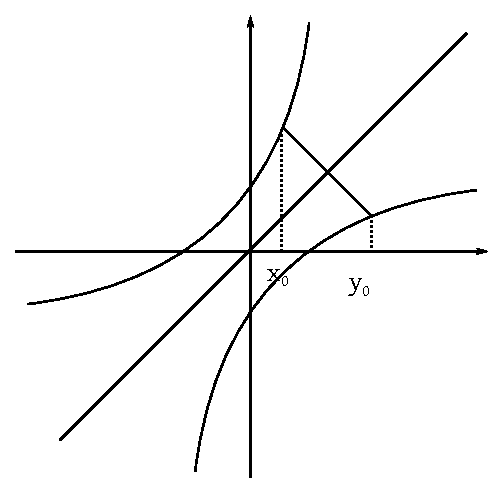
\includegraphics{img/geometric-exp-proof.pdf}
    \caption{A geometric proof of differentiability}
    \label{img:geo-diff}
  \end{center}
\end{figure}
\begin{proof}
  \begin{description}
    \item[First approach]
      Let $x > 0$, $x_n \to x$ with $x_n \neq x$, $x_n > 0$.
      Let $\xi_n = \ln(x_n)$ and $\xi = \ln(x) \Rightarrow \xi_n \neq \xi$.
      \[ e^{\xi_n} = x_n \qquad e^\xi = x \qquad \xi_n \to \xi \]
      Then it holds that
      \[ \lim_{n\to\infty} \frac{\ln(x_n) - \ln(x)}{x_n - x} = \lim_{n\to\infty} \frac{\xi_n - \xi}{e^{\xi_n} - e^\xi} \]
      \[
        = \lim_{n\to\infty} \frac{1}{\frac{e^{\xi_n} - e^\xi}{\xi_n - \xi}}
        = \frac{1}{\underbrace{\lim_{n\to\infty} \frac{e^{\xi_n} - e^\xi}{\xi_n - \xi}}_{(e^\xi)' = e^\xi}}
        = \frac1{e^\xi} = \frac1x
      \]
    \item[Second approach using chain rule]
      Compare with Figure~\ref{img:geo-diff}.
      \[ (f^{-1})'(y_0) = \frac{1}{f'(f^{-1}(y_0))} \]
      \[ f(f^{-1}(y)) = y \Rightarrow f(f^{-1}) f(f^{-1}(y)) = y = f'(f^{-1}(y)) \cdot (f^{-1})'(y) = 1 \]
      \[ \Rightarrow (f^{-1})'(y) = \frac{1}{f'(f^{-1}(y))} \text{ for } f(x) = \exp(x) \]
      \[ \Rightarrow (\ln)'(y) = \frac{1}{\exp(\ln(y))} = \frac{1}{y} \]

      \[ f(f^{-1}(y)) = y \]
      \[ f'(f^{-1}(y)) \cdot (f^{-1}) \]
      \[ = (f^{-1})'(y) = \frac{1}{f'(f^{-1}(y))} \]
      again for $f(x) = \exp(x)$.
    \item[Third approach]
      Let $x > 0$.
      \[ 0 = \ln(1) = \ln\left(x \cdot \frac1x\right) = \ln(x) + \ln\left(\frac1x\right) \]
      \[ \Rightarrow \ln\left(\frac1x\right) = -\ln(x) \]

      Let $x,y > 0$. Then it holds that
      \[ \ln{\frac{x}{y}} = \ln(x) - \ln(y) \]
      because $\ln\frac{x}{y} = \ln(x \cdot \frac1y) = \ln(x) - \ln(y)$.
  \end{description}
\end{proof}

\subsection{Extension of the functional equation of logarithm}
%


\subsection{A different proof for the derivative of logarithm}
%
\begin{proof}
  \[
    [\ln(x)]'
    = \lim_{h\to0} \frac{\ln(x + h) - \ln(x)}{h}
    = \lim_{h\to0} \frac{\ln\left(\frac{x+h}{x}\right)}{h}
    = \lim_{h\to0} \frac{\ln\left(1 + \frac{h}{x}\right)}{x \cdot \frac hx}
  \] \[
    = \frac1x \cdot \lim_{h\to0} \frac{\ln\left(1 + \frac{h}{x}\right)}{\frac{h}{x}}
    \text{ where } \frac hx \to 0
  \]
  $1 + \frac{h}{x} = w$ then it holds that $h \to 0 \Rightarrow w \to 1$.
  \[ \frac{h}{x} = w - 1 \]
  \[ \lim_{h\to0} \frac{\ln\left(1 + \frac{h}{x}\right)} = \lim_{h\to0} \frac{\ln(w)}{w - 1} = 1 \]
\end{proof}

\begin{rem}
  The exponential function can be defined from $\mathbb C$ to $\mathbb C$.
  \[ \exp: \mathbb C \to \mathbb C \]
  It is not possible to define the logarithm \emph{continuously} in entire $\mathbb C$
  (or $\mathbb C \setminus \set{0}$). We can only define a continuous inverse function
  of $\exp$ in $\mathbb C \setminus \set{x \in \mathbb R: x \leq 0}$
\end{rem}

\begin{figure}[!h]
  \begin{center}
    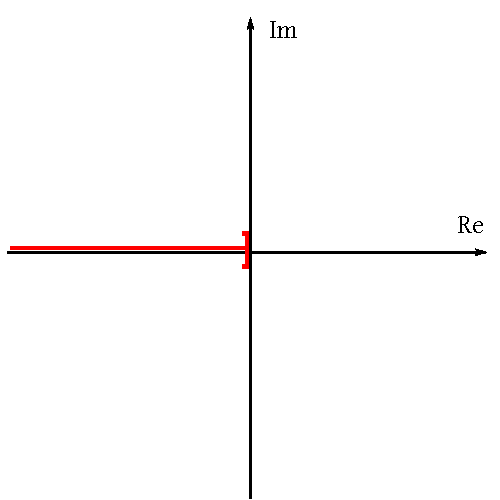
\includegraphics{img/continuous-exp-in-C.pdf}
    \caption{Continuous exponential function in $\mathbb C$}
  \end{center}
\end{figure}

\meta{lecture}{3rd of March 2016}{Wolfgang Ring}

\subsection{Further remarks on differential calculus}

\begin{theorem}
  Let $f: I \to \mathbb R$ be strictly monotonically increasing (or s. m. decreasing)
  where $I$ is an interval. Then $f^{-1}: f(I) \to \mathbb R$ is defined and the inverse function.

  Let $f$ in $x_0 \in I$ be differentiable and $f'(x_0) \neq 0$. Then $f^{-1}$ is in $y_0 = f(x_0)$
  differentiable and it holds that
  \[ (f^{-1})'(y_0) = \frac{1}{f'(x_0)} = \frac{1}{f'(f^{-1}(y_0))} \]
\end{theorem}

\begin{proof}
  Let $y_n \to y_0$ and $y_n \in f(I)$; $y_0 = f(x_0)$; $y_0 \in f(I)$; $y_n = f(x_n)$.
  $y_n \neq y_0 \Rightarrow x_n \neq x_0$.
  \[ \lim_{n\to\infty} \frac{f^{-1}(y_n) - f^{-1}(y_0)}{y_n - y_0} \]
  \[
    = \lim_{n\to\infty} \frac{x_n - x_0}{f(x_n) - f(x_0)}
    = \frac{1}{\lim_{n\to\infty} \underbrace{\frac{f(x_n) - f(x_0)}{x_n - x_0}}}_{\text{ex} = f'(x_0)} = \frac{1}{f'(x_0)}
  \]
\end{proof}

\begin{lemma}
  \label{lemma:const-diff}
  Let $f: I \to \mathbb R$ where $I$ is some interval. Then it holds that
  \[ f = \text{ const} \Leftrightarrow f \text{ is differentiable in $I$ and } f'(x) = 0 \forall x \in I \]
\end{lemma}
\begin{proof}
  \begin{description}
    \item[$\Rightarrow$]
      Immediate.
    \item[$\Leftarrow$]
      Let $f$ be differentiable and $f' \equiv 0$.
      Assume $f$ is not constant. Then there exist $x_1, x_2 \in I$, $x_1 \neq x_2$
      and $f(x_1) \neq f(x_2)$. Without loss of generality, $x_1 < x_2$.
      The Intermediate Value Theorem states that
      \[ \exists \xi \in (x_1, x_2) \subseteq I: f'(\xi) = \frac{f(x_2) - f(x_1)}{x_2 - x_1} \neq 0 \]
      This is a contradiction to the assumption that $f' \equiv 0$.
  \end{description}
\end{proof}

\index[English]{Primitive}
\index[German]{\foreignlanguage{ngerman}{Stammfunktion}}
\begin{defi}
  Let $I$ be an interval, $f: I \to \mathbb R$.
  A function $F: I \to \mathbb R$ is called \emph{primitive} or \emph{antiderivative} of $f$
  if $F$ is differentiable and
  \[ \forall x \in I: F'(x) = f(x) \]
\end{defi}
\begin{lemma}
  Let $f: I \to \mathbb R$. Let $F_1$ and $F_2$ be two primitive functions of $f$.
  Then it holds that $F_1 - F_2 = \text{const}$.
\end{lemma}
\begin{proof}
  $F_1$, $F_2$ are differentiable.
  \[ (F_1 - F_2)'(x) = F_1'(x) - F_2'(x) = f(x) - f(x) = 0 \]
  \[ \xRightarrow{\text{Lemma~\ref{lemma:const-diff}}} F_1 - F_2 = \text{ const} \]
\end{proof}

\begin{theorem}
  Let $I$ be an interval.
  Let $(f_n)_{n\in\mathbb N}$ be a sequence of differentiable functions in $I$.
  \[ f_n: I \to \mathbb R \text{ differentiable} \]
  Furthermore let $f: I \to \mathbb R$.
  It holds that,
  \begin{enumerate}
    \item
      $\forall x \in I$ let $f(x) = \lim_{n\to\infty} f_n(x)$
      ($f_n \to f$ pointwise)
    \item
      for every $x \in I$ let $(f'_n(x))_{n\in\mathbb N}$ be convergent
      (hence $\varphi(x) = \lim_{n\to\infty} f_n'(x)$ exists for every $x$)
    \item
      $\forall \varepsilon > 0 \exists N \in \mathbb N$ such that
      \[ n \geq N \Rightarrow \abs{(f_n - f)(u) - (f_n - f)(v)} \leq \varepsilon \abs{u - v} \forall u,v \in I \]
      Then $f$ is differentiable in $I$ and it holds that $f'(x) = \varphi(x) = \lim_{n\to\infty} f'_n(x)$.
      \[ f'(x) = [\lim_{n\to\infty} f]'(x) \]
  \end{enumerate}
\end{theorem}
\begin{proof}
  Let $x_0 \in I$ and $x \in I$. Let $\varepsilon > 0$ arbitrary.
  \[ \abs{\frac{f(x) - f(x_0)}{x - x_0} - \varphi(x_0)} \]
  \[ = \abs{\frac{f(x) - f(x_0)}{x - x_0} - \lim_{n\to\infty} f_N'(x_0)} \]
  \[ = \abs{\frac{f(x) - f(x_0)}{x - x_0} - f'_N(x_0)} + \abs{f'_N(x_0) - \lim_{n\to\infty} f'_n(x_0)} \forall N \in \mathbb N \]
  \[
    \leq \abs{\frac{f(x) - f(x_0)}{x - x_0} - \frac{f_N(x) - f_N(x_0)}{x - x_0}}
  \] \[
    + \abs{\frac{f_N(x) - f_N(x_0)}{x - x_0} - f'_N(x_0)}
    + \abs{f'_N(x_0) - \varphi(x_0)}
  \]

  \begin{description}
    \item[1st term]
      \[
        \abs{\frac{(f(x) - f_N(x)) - (f(x_0) - f_N(x_0))}{x - x_0}}
        = \abs{\frac{(f - f_N)(x) - (f - f_N)(x_0)}{x - x_0}}
      \] \[
        \leq \frac\varepsilon3 \frac{\abs{x - x_0}}{\abs{x - x_0}}
        \stackrel{\text{condition 3}}{=} \frac{\varepsilon}{3}
      \]
      for sufficiently large $N$.
    \item[3rd term]
      $\abs{f'_N(x_0) - \varphi(x)} < \frac{\varepsilon}{3}$ for sufficiently large $N$.
  \end{description}

  Now let $N$ be fixed (with a value such that the first and third term is less than $\frac\varepsilon3$).

  \begin{description}
    \item[2nd term]
      \[ \abs{\frac{f_N(x) - f_N(x_0)}{x - x_0}} - f'_N(x_0) \]
  \end{description}

  Differentiability of $f_N$:
  Therefore for $\abs{x - x_0} < \delta$.
  \[
    \abs{\frac{f(x) - f(x_0)}{x - x_0} - \varphi(x_0)}
    < \frac\varepsilon3 + \frac\varepsilon3 + \frac\varepsilon3
    = \varepsilon
  \]
  $f$ is differentiable in $x_0$ and $f'(x_0) = \varphi(x_0)$.
\end{proof}

\begin{theorem}
  Let $f_n: I \to \mathbb R$ and $f: I \to \mathbb R$ ($n \in \mathbb N$)
  and $f_n$ is differentiable in $I$.

  Assumption:
  \begin{enumerate}
    \item $f_n \to f$ converges pointwise in $I$
      (like the first statement in the previous Theorem)
    \item There exists $g: I \to \mathbb R$ such that
      $f'_n \to g$ is continuous in $I$
  \end{enumerate}
  Then $f$ is differentiable in $I$ and it holds that
  \[ f'(x_0) = g(x_0) \quad \forall x_0 \in I \]
\end{theorem}

\meta{lecture}{4th of March 2016}{Wolfgang Ring}

\begin{theorem}[Reminder of theorem]
  \label{thm:diff-conv}
  Let $(f_n)_{n\in\mathbb N}$ be a sequence of functions in $I$ and
  let $f_n$ be differentiable $\forall n \in \mathbb N$. Furthermore,
  \begin{itemize}
    \item $f_n \to f$ pointwise
    \item $f'_n(x) \to \varphi(x)$ for every $x$
    \item $\forall \varepsilon > 0 \forall u,v \in I \exists N: n \geq N
      \Rightarrow \abs{(f_n - f)(u) - (f_n - f)(v)} < \varepsilon \abs{u - v}$
  \end{itemize}
  Then it holds that $f$ is differentiable and $f'(x) = \varphi(x) \forall x \in I$.
\end{theorem}

Conclusion:
\begin{theorem}
  \label{thm:concl}
  Let $f_n$ and $f$ be differentiable as in Theorem~\ref{thm:diff-conv}:
  $f_n: I \to \mathbb R$ and $f: I \to \mathbb R$ and it holds that
  \begin{itemize}
    \item $f_n \to f$ pointwise in $I$ for $n \to \infty$
    \item $\exists g: I  \to \mathbb R$ such that $f'_n \to g$ is \emph{uniform} in $I$,
      hence $\forall \varepsilon > 0 \exists N \in \mathbb N:
      n \geq N \land x \in I \Rightarrow \abs{f'_n(x) - g(x)} < \varepsilon$
  \end{itemize}
  Then $f$ is differentiable in $I$ and $f'(x) = g(x) \forall x \in I$.
\end{theorem}
\begin{proof}
  We check whether the two conditions lead to the conditions of Theorem~\ref{thm:diff-conv}.

  We look at the conditions of Theorem~\ref{thm:diff-conv}:
  \begin{itemize}
    \item[2.] Uniform convergences of $f'_n \to g$ implies pointwise convergence
      \[ \forall x \in I: f'_n(x) \to g(x) \]
    \item[3.] From uniform convergence of $f'_n \to g$ it follows that
      Let $\varepsilon > 0$ be arbitrary and $N$ is sufficiently large enough, such that
      $\forall n \geq N$ and $\forall x \in I$:
      \[ \abs{f_n'(x) - g(x)} < \frac\varepsilon2 \]
      Choose $n,m \geq N$ and $x \in I$ arbitrary. Then it holds that
      \[ \abs{f'_n(x) - f'_m(x)} = \abs{f'_n(x) - g(x) + g(x) - f'_m(x)} \]
      \[ \leq \abs{f'_n(x) - g(x)} + \abs{g(x) - f'_m(x)} < \frac\varepsilon2 + \frac\varepsilon2 = \varepsilon \]
      So $(f_n)_{n\in\mathbb N}$ is a uniform Cauchy sequence.

      Let $\varepsilon > 0$ be arbitrary and $N$ such that $n,m \geq N$ and $x \in I$:
      \[ \abs{f'_n(x) - f'_m(x)} < \varepsilon \]

      Consider the third condition of Theorem~\ref{thm:diff-conv}. Let $u,v \in I$
      \[ \abs{(f - f_n)(u) - (f - f_n)(v)} = \lim_{m\to\infty} \abs{(f_m - f_n)(u) - (f_m - f_n)(v)} \]
      where $(f_m - f_n)$ and $(f_m - f_n)$ is differentiable. Then according to the
      mean value theorem of differential calculus (dt. Mittelwertsatz der Differentialrechnung)
      \begin{align*}
        &= \lim_{m\to\infty} \abs{(f_m - f_n)'(\xi_{m,n}) \cdot (u - v)} \\
        &= \lim_{m\to\infty} \abs{f'_m(\xi_{m,n}) - f'_n(\xi_{m,n})} \cdot \abs{u - v}
      \end{align*}
      For $m \geq N$:
      \[ \leq \varepsilon \cdot \abs{u - v} \]
      So the third condition of Theorem~\ref{thm:diff-conv} is satisfied.
  \end{itemize}
\end{proof}

\begin{figure}[!h]
  \begin{center}
    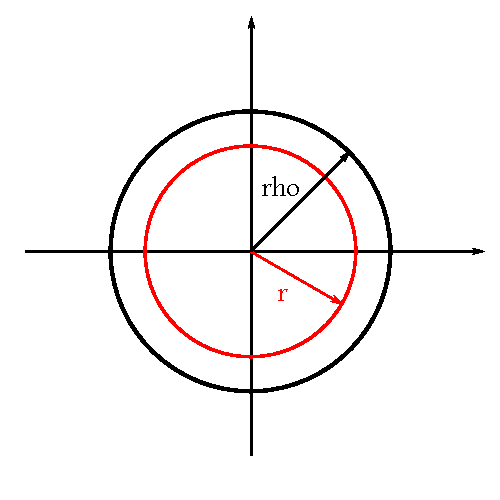
\includegraphics{img/convergence_radius.pdf}
    \caption{Convergence radius}
    \label{fig:convr}
  \end{center}
\end{figure}


\begin{rem}[An application of Theorem~\ref{thm:concl}]
  Let $P(z) = \sum_{k=0}^\infty a_k z^k$ be a power series with convergence radius $\rho(P)$ with
  \[ \rho(P) = \frac1L \qquad L = \limsup_{n\to\infty} \sqrt[n]{\abs{a_n}} \]
  \[ P_n(z) = \sum_{k=0}^n a_k z^k \qquad \text{\dots $n$-th partial sum} \]
  Let $r < \rho(P)$. Then it holds that $P_n(z) \to P(z)$ uniform in $\overline{B(0,r)}$~\footnote{Where overline means \enquote{closed}}.
  \[ P_n(x) \to P(x) \forall x \in [-r, r] \]

  Compare with Figure~\ref{fig:convr}.

  \[ P'_n(x) = \sum_{k=0}^n a_k k \cdot x^{k-1} = \sum_{j=0}^{n-1} a_{j+1} (j + 1) x^j \]
  is the $n-1$-th partial sum.
  \[ Q(z) = \sum_{j=0}^\infty a_{j+1} (j + 1) z^j \]
  Convergence radius of $Q$?
  \[ \tilde{L} = \limsup_{j\to\infty} \sqrt[j]{a_{j+1}} \cdot \sqrt[j]{j + 1} = \limsup_{j \to \infty} \abs{a_{j+1}}^{\frac{j+1}{j} \cdot \frac{1}{j+1}} \cdot (j+1)^{\frac{j+1}{j} \cdot \frac{1}{j+1}} \]
  \[
    = \limsup_{j\to\infty} \underbrace{\left(\abs{a_{j+1}}^{\overbrace{\frac{1}{j+1}}^{\to 1}}\right)^{\frac{j+1}{j}}}_{L^1 = L}
    \cdot \underbrace{\lim_{j\to\infty} \left[(j+1)^{\frac{1}{j+1}}\right]^{\frac{j+1}{j}}}_{1^1}
    = L
  \]
  In conclusion we have $\tilde L = L$ and $\rho(Q) = \frac1{L} = \rho(P)$.
  So $P'_n(z) = \sum_{k=1}^n k \cdot a_k z^{k-1}$ uniformly convergent in $\overline{B(0,r)}$ for $r<\rho$
  and therefore also uniformly convergent  in $[-r,r]$.

  From Theorem~\ref{thm:diff-conv} (or \ref{thm:concl}?) it follows that $P(x)$ is differentiable % TODO: or?
  in $[-r,r]$ and $P'(x) = \sum_{k=1}^\infty k \cdot a_k \cdot x^{k-1}$.

  Let $\abs{x} < \rho(P)$. Let $r = \frac12 (\abs{x} + \rho(P))$, then it holds that
  $x \in [-r, r]$ and $P$ is differentiable in point $x$ with
  \[ P'(x) = \sum_{k=1}^\infty k \cdot a_k \cdot x^{k-1} \]
\end{rem}

\begin{lemma}
  Let $P(z) = \sum_{k=0}^\infty a_k z^k$ be a power series with convergence radius $\rho(P) > 0$.
  Let $x \in (-\rho(P), \rho(P))$. Then $P$ is differentiable in $x$ and it holds that
  \[ P'(x) = \sum_{k=1}^\infty k \cdot a_k \cdot x^{k-1} \]

  Furthermore the power series $\sum_{k=1}^\infty k \cdot a_k \cdot x^{k-1}$ is uniformly convergent
  in every interval $[-r, r]$ with $0 < r < \rho(P)$.
\end{lemma}

\subsection{About logarithm functions}
%
We consider the power series
\[ g(z) = \sum_{k=1}^\infty \frac{z^k}{k} \]
\[ \rho(g) = \frac1L \text{ with } L = \limsup_{k\to\infty} \sqrt[k]{\frac1k} = \frac{1}{\lim_{k\to\infty} \sqrt[k]{k}} = 1 \]
So it holds that $\rho(g) = 1$.

Apply the previous theorem, followingly $g$ is differentiable in $(-1,1)$ and it holds that
\[ g'(x) = \sum_{k=1}^\infty \frac{k}{k} x^{k-1} = \sum_{j=0}^\infty x^j = \frac1{1 - x} \]

Remark:
\[ \left[-\ln(1 - x)\right]' = -\frac{1}{1 - x} \cdot (-1) = \frac1{1 - x} \]
\[ \Rightarrow \sum_{k=1}^\infty \frac{x^k}{k} + \ln(1 - x) = \text{ constant} \]
Let $x = 0$ (we determine the constant for this $x=0$):
\[ 0 + 0 = 0 = \text{ constant} \]
\[ \Rightarrow \ln(1 - x) = -\sum_{k=1}^\infty \frac{x^k}{k} \qquad \text{ for } \abs{x} < 1 \]

Let $x \in (-1,1) \Rightarrow -x \in (-1,1)$.
\[ \Rightarrow \ln(1 - (-x)) = \ln(1 + x) = -\sum_{k=1}^\infty \frac{(-x)^k}{k} \]
\[ = \sum_{k=1}^\infty \frac{(-1)^{k-1} \cdot x^k}{k} = x - \frac{x^2}{2} + \frac{x^3}{3} - \frac{x^4}{4} + \ldots \]

\index[English]{Logarithmic series}
\index[German]{\foreignlanguage{ngerman}{Logarithmische Reihe}}
Therefore: We introduce \emph{logarithmic series}:
\[ \ln(1 - x) = -\sum_{k=1}^\infty \frac{x^k}{k} \]
\[ \ln(1 + x) = \sum_{k=1}^\infty \frac{(-1)^{k-1} x^k}{k} \]
\[
  \ln\left(\frac{1 + x}{1 - x}\right)
  = \ln(1 + x) - \ln(1 - x)
  = 2 \sum_{l=1}^\infty \frac{x^{2l - 1}}{2l - 1}
  \quad \text{ for } x \in (-1,1)
\]

\begin{figure}[!h]
  \begin{center}
    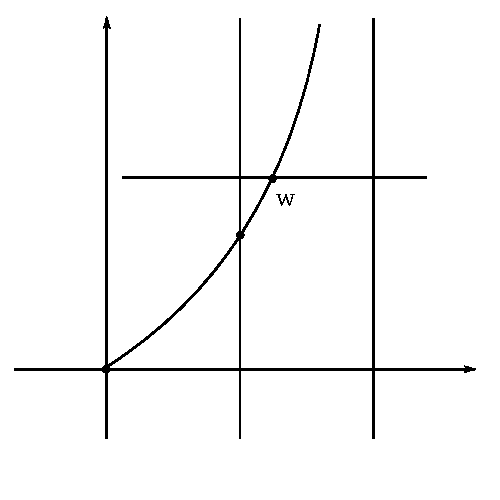
\includegraphics{img/1x_1-x.pdf}
    \caption{Plot of $\frac{1+x}{1-x}$}
    \label{img:1x-1x}
  \end{center}
\end{figure}

\[ f(x) = \frac{1 + x}{1 - x} \]
Compare with Figure~\ref{img:1x-1x}.
\[ f'(x) = \frac{1 - (-1)}{(1 - x)^2} = \frac{2}{(1 - x)^2} > 0 \quad \text{ in } (-1, 1) \]
Solve $\frac{1 + x}{1 - x} = w$ for $x$.

\[ \Rightarrow 1 + x  = w - wx \]
\[ x (1 + w) = w - 1 \]
\[ x = \frac{w - 1}{w + 1} \]

\[ \ln(w) = 2 \sum_{l=1}^\infty \frac{x^{2l-1}}{2l - 1} \]

\section{Trigonometic functions}

We define trigonometic functions using the exponential function in $\mathbb C$.

Let $t \in \mathbb R$.
\[ e^{it} = \sum_{k=0}^\infty \frac{(it)^k}{k!} = \lim_{n\to\infty} \left(\underbrace{1}_{\mathbb R} + \underbrace{\frac{it}{n}}_{i \mathbb R}\right)^n \]
\[
  e^{-it}
    = \lim_{n\to\infty} \left(1 - \frac{it}{n}\right)^n
    = \lim_{n\to\infty} \left[\overline{\left(1 + \frac{it}{n}\right)}\right]^n
\] \[
  = \lim_{n\to\infty} \overline{\left(1 + \frac{it}{n}\right)^n}
  = \overline{\lim_{n\to\infty} \left(1 + \frac{it}{n}\right)^n}
  = e^{it}
\] \[
  \abs{e^{it}}^2 = e^{it} \cdot \overline{e^{it}} = e^{it} \cdot e^{-it}
\] \[
  e^{it - it} = e^0 = 1
\]
So it holds that $\forall t \in \mathbb R$:
\[ \abs{e^{it}} = 1 \]
So $e^{it}$ lies inside the complex unit circle. Compare with Figure~\ref{img:unitc}.

\begin{figure}[!h]
  \begin{center}
    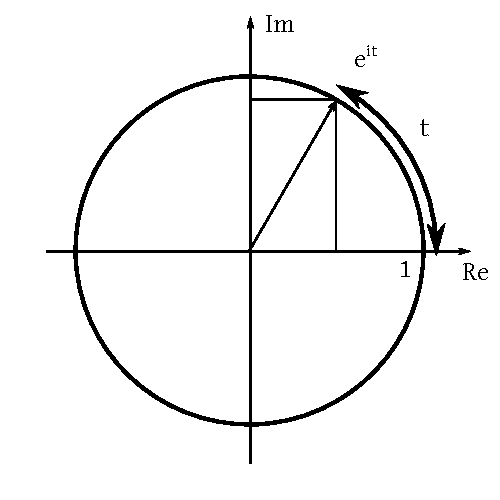
\includegraphics{img/unitcircle_in_C.pdf}
    \caption{Unit circle in $C$ with $t$}
    \label{img:unitc}
  \end{center}
\end{figure}

\index[English]{Sine function}
\index[German]{\foreignlanguage{ngerman}{Sinusfunktion}}
\index[English]{Cosine function}
\index[German]{\foreignlanguage{ngerman}{Cosinusfunktion}}
We define the cosine function $\cos: \mathbb R \to \mathbb R$ as
\[ \cos(t) = \Re(e^{it}) \]
and the sine function $\sin: \mathbb R \to \mathbb R$ as
\[ \sin(t) = \Im(e^{it}) \]

The following relations hold:
\begin{enumerate}
  \item $e^{it} = \cos(t) + i \cdot \sin(t)$ (Euler's identity)
  \item $\abs{e^{it}}^2 = 1 = (\cos{t})^2 + (\sin{t})^2$
  \item \[ \Re(z) = \frac12 (z + \overline{z}) \]
    \[ \Rightarrow \cos(t) = \Re(e^{it}) = \frac12 \left(e^{it} + e^{-it}\right) \]
    \[ \Im(z) = \frac1{2i} [z - \overline{z}] \]
    \[ \sin(t) = \Im(e^{it}) = \frac{1}{2i} \left[e^{it} - e^{-it}\right] \]
  \item
    \[ e^{-it} = \overline{e^{it}} = \cos{t} - i \cdot \sin{t} \]
\end{enumerate}

We use property 3 to extend the domain of sine and cosine:
\begin{defi}
  Let $z \in \mathbb C$. We define $\sin: \mathbb C \to \mathbb C$
  and $\cos: \mathbb C \to \mathbb C$ by
  \[ \cos(z) = \frac12 \left[e^{iz} + e^{-iz}\right] \]
  \[ \sin(z) = \frac1{2i} \left[e^{iz} - e^{-iz}\right] \]
\end{defi}

\meta{lecture}{8th of March 2016}{Wolfgang Ring}

\begin{figure}
  \begin{center}
    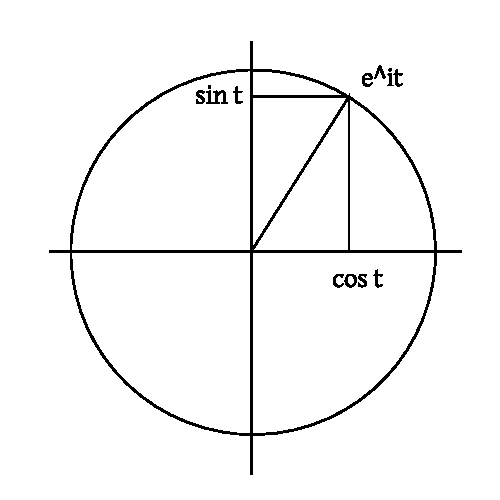
\includegraphics{img/complex_unit.pdf}
    \caption{The trigonometric values $\sin{t}$ and $\cos{t}$ in the unit circle}
    \label{img:cossin}
  \end{center}
\end{figure}
%
Compare with Figure~\ref{img:cossin}.

\begin{align*}
  t \in \mathbb R:
    \cos{t} = \Re(e^{it}) = \frac12 (e^{it} + e^{it}) \\
    \sin{t} = \Im(e^{it}) = \frac{1}{2i} (e^{it} - e^{-it})
\end{align*}

\begin{align*}
  z \in \mathbb C:
    \cos{z} &= \frac12 (e^{iz} + e^{-iz}) \\
    \sin{z} &= \frac{1}{2i} (e^{iz} - e^{-iz})
\end{align*}

Properties:
\begin{align*}
  \cos{-z} &= \frac12 (e^{i(-z)} + e^{-i}(-z)) = \cos{z} \\
  \intertext{$\cos{z}$ is even}
  \sin{-z} &= \frac1{2i} (e^{-iz} - e^{iz}) = -\sin{z}
  \intertext{$\sin{z}$ is odd}
\end{align*}

The cosine function in the complex space is even.

\subsection{Series representation of trigonometric functions}

\begin{lemma}[Addition of series of absolute convergence]
  Let $(a_n)_{n\in\mathbb N}$, $(b_n)_{n\in\mathbb N}$ be complex sequences
  and the series $\sum_{n=0}^\infty a_n$ and $\sum_{n=0}^\infty b_n$ are absolute
  convergent with series value $\sum_{n=0}^\infty a_n = a$ and $\sum_{n=0}^\infty b_n = s'$.

  Then $\sum_{n=0}^\infty (a_n + b_n)$ is absolute convergent with sum $s + s'$.
\end{lemma}
\begin{proof}[series sum]
  Absolute convergence.
  Show that $\sum_{k=0}^n = \abs{a_k + b_k} = t_n$ and $(t_n)_{n\in\mathbb N}$ is bounded.

  Follows immediately, because
  \[ \sum_{k=0}^n \abs{a_kk + b_k} \leq \underbrace{\sum_{k=0}^n \abs{a_k}}_{\text{bounded}} + \underbrace{\sum_{k=0}^n \abs{b_k}}_{\text{bounded}} \]
\end{proof}

\begin{ex}[Application]
  Let $P(z) \coloneqq \sum_{k=0}^\infty a_k z^k$ and $Q(z) \coloneqq \sum_{k=0}^\infty b_k z^k$ be power series.
  Both are convergent in $B(0, \delta)$. Then also $\sum_{k=0}^\infty (a_k + b_k) z^k$ is convergent in $B(0,\delta)$
  and it holds that $\sum_{k=0}^\infty (a_k + b_k) z^k = P(z) + Q(z)$.
\end{ex}

\subsection{Application to trigonometric functions}
%
\[ e^{iz} = \sum_{k=0}^\infty \frac{(iz)^k}{k!} = \sum_{k=0}^\infty i^k \cdot \frac{z^k}{k!} \]
\[ i^0 = 1 \qquad i^1 = i \qquad i^2 = -1 \qquad i^3 = -i \qquad i^4 = 1 = i^0 \qquad i^5 = i \qquad \ldots \]
\[ \Rightarrow = 1 + i \frac{z}{1!} - \frac{z^2}{2!} - i \frac{z^3}{3!} + \frac{z^4}{4!} + i \frac{z^5}{5!} - \frac{z^6}{6!} \]

\[ e^{-iz} = \sum_{k=0}^\infty \frac{(-iz)^k}{k!} = \sum_{k=0}^\infty (-i)^k \frac{z^k}{k!} \]
\[ (-i)^0 = 1 \qquad (-i)^1 = -i \qquad (-i)^2 = -1 \qquad (-i)^3 = i \qquad (-i^4) = 1 \qquad \ldots \]
\[ \Rightarrow = 1 - i \frac{z}{1!} - 1\frac{z^2}{2!} + i \frac{z^3}{3!} + \frac{z^4}{4!} - i \frac{z^5}{5!} - \frac{z^6}{6!} + \ldots \]

\[ \frac12 (e^{iz} + e^{-iz}) = 1 - \frac{z^2}{2!} + \frac{z^4}{4!} - \frac{z^6}{6!} + \frac{z^8}{8!} - \frac{z^{10}}{10!} + \ldots \]

Followingly,
\begin{align*}
  \cos{z} &= 1 - \frac{z^2}{2!} + \frac{z^4}{4!} - \frac{z^6}{6!} + \frac{z^8}{8!} - \ldots \\
          &= \sum_{l=0}^\infty (-1)^l \frac{z^{2l}}{(2l)!} \text{ convergent in } \mathbb C \\
  \sin{z} &= \frac1{2i}(e^{iz} - e^{-iz}) = z - \frac{z^3}{3!} + \frac{z^5}{5!} - \frac{z^7}{7!} + \frac{z^9}{9!} + \ldots \\
          &= \sum_{l=0}^\infty (-1)^l \frac{z^{2l + 1}}{(2l+1)!}
\end{align*}

\subsection{Functional equations of trigonometric functions}
%
\begin{theorem}[Addition and substraction theorems]
  We derive them directly:

  Let $z,w \in \mathbb C$.
  \begin{align*}
    e^{z+w} &= e^z \cdot e^w = (\cos{z} + i \cdot \sin{z}) (\cos{w} + i \cdot \sin{w}) \\
    \intertext{but also}
            &= (\cos(z + w) + i \sin(z + w)) \\
            &\Rightarrow = (\cos{z} \cdot \cos{w} - \sin{z} \cdot \sin{w}) + i (\cos{z} \cdot \sin{w} + \sin{z} \cdot \cos{w})
  \end{align*}

  Analogously,
  \begin{align*}
    e^{-(z+w)} &= e^{-z} \cdot e^{-w} = (\cos(-z) + i \cdot \sin(-z)) (\cos(-w) + i \cdot \sin(-w)) \\
               &= \cos{z} \cdot \cos{w} - \sin{z} \sin{w} + i \left(-\cos{z} \sin{w} - \cos{w} \sin{z}\right) \\
    \intertext{but also}
            &= (-\cos(z + w) + i \sin(-(z + w))) \\
            &\Rightarrow = \cos{(z + w)} - i \sin(z + w)
  \end{align*}

  \begin{align*}
    \intertext{Addition:} \\
    2 \cos(z+w) &= 2 (\cos{z} \cdot \cos{w} - \sin{z} \sin{w}) \\
    \Rightarrow \cos(z + w) &= \cos{z} \cos{w} - \sin{z} \sin{w}
    \intertext{Subtraction:}
    \Rightarrow \sin(z + w) &= \cos{z} \sin{w} + \sin{z} \cos{w} \forall z,w \in \mathbb C
  \end{align*}

  Variations: $w \leftrightarrow -w$
  \begin{align*}
    \cos(z - w) &= \cos{z} \cdot \underbrace{\cos{w}}_{=\cos(-w)} + \sin{z} \underbrace{\sin{w}}_{=-\sin(-w)} \\
    \sin(z - w) &= -\cos{z} \cdot \sin(w) + \sin(z) \cos(w)
  \end{align*}
\end{theorem}

\begin{cor}
  \[ z = \frac12 (z + w) + \frac12 (z - w) \]
  \[ \Rightarrow \cos{z} = \cos{\frac{z + w}{2}} \cos{\frac{z - w}{2}} - \sin{\frac{z + w}{2}} \sin{\frac{z - w}{2}} \]
  \[ w = \frac12 (w + z) + \frac12 (w - z) = \frac12 (z + w) - \frac12 (z - w) \]
  \[ \cos{w} = \cos{\frac{z + w}{2}} \cdot \cos{\frac{z - w}{2}} + \sin{\frac{z + w}{2}} \cdot \sin{\frac{z - w}{2}} \]
  \[ \cos{z} - \cos{w} = -2 \sin{\frac{z + w}{2}} \sin{\frac{z - w}{2}} \]
  Analogously,
  \[ \sin{z} - \sin{w} = 2 \cos{\frac{z + w}{2}} \cdot \cos{\frac{z - w}{2}} \]
\end{cor}

We consider
\begin{align*}
  \lim_{\substack{z \to 0 \\ z \neq 0}} \frac{\sin{z}}{z}
    &= \lim_{z \to 0} \frac{1}{2i} \left(\frac{e^{iz} - e^{-iz}}{z}\right) \\
    &= \lim_{z \to 0} e^{-iz} \left(\frac{e^{2iz} - 1}{2iz}\right) \\
    &= \underbrace{\lim_{z \to 0} e^{-iz}}_{=e^0 = 1} \cdot \underbrace{\lim_{z \to 0} \frac{e^{2iz} - 1}{2iz}}_{\substack{e = 2iz; z \to 0 \Leftrightarrow w = 0 \\ \lim_{w \to 0} \frac{e^w - 1}{w} = 1}}
\end{align*}

So it holds that
\[ \lim_{z\to0} \frac{\sin{z}}{z} = 1 \]

\subsection{Trigonometric functions for real arguments}
%
Subtitled \enquote{definition of $\pi$} and \enquote{periodicity}.

Let $x \in \mathbb R$.
\[ \cos{x} = \overbrace{1}^{=c_0} - \overbrace{\frac{x^2}{2}}^{=c_1} + \overbrace{\frac{x^4}{24}}^{=c_2} - \overbrace{\frac{x^6}{720}}^{=c_3} + \overbrace{\frac{x^8}{40320}}^{=c_4} - \ldots \]
\[ \sin{x} = \underbrace{x}_{=s_0} - \underbrace{\frac{x^3}{6}}_{=s_1} + \underbrace{\frac{x^5}{120}}_{=s_2} - \underbrace{\frac{x^7}{5040}}_{=s_3} + \ldots \]

\[ c_n = \frac{x^{2k}}{(2k)!} \qquad s_k = \frac{x^{2k+1}}{(2k+1)!} \]

For $x \in [0,2]$ and $k \geq 1$ it holds that
\[ \abs{\frac{c_{k+1}}{c_k}} = \abs{\frac{x^2}{(2k + 2)(2k + 1)}} \leq \frac{4}{3 \cdot 4} = \frac13 \]
so $(c_k)_{k\geq1}$ is strictly monotonically decreasing.

Leibniz criterion:
\[ 1 - \frac{x^2}{2} < \cos{x} < 1 - \frac{x^2}{2} + \frac{x^4}{24} \]
for $x \in (0,2]$.

Similarly for $x \in (0,2]$:
\[ \abs{\frac{s_{k+1}}{s_k}} = \abs{\frac{x^2}{(2k + 2)(2k + 3)}} \leq \frac{4}{4 \cdot 5} = \frac15 < 1 \]
So the Leibniz criterion tells us that
\[ x - \frac{x^3}{6} < \sin{x} < x \quad \text{ in } [0, 2] \]
So it holds that
\[ \cos(0) = 1 \]
\[ \cos(2) < 1 - 2 + \frac{16}{24} = -1 + \frac23 = -\frac13 \]
Intermediate value theorem (power series is continuous):
\[ \exists \xi \in (0,2) \text{ with } \cos(\xi) = 0 \]
Let $0 \leq w < z \leq 2$,
\[ 0 < \frac{z-w}{2} \leq \frac{z+w}{2} < \frac{z + z}{2} \leq 2 \]

Let $x \in (0,2]$, then it holds that
\[ \sin(x) > x - \frac{x^3}{6} = \underbrace{x}_{>0} \underbrace{\left(1 - \frac{x^2}{6}\right)}_{>1 - \frac46 = \frac13 > 0} > 0 \]
So it holds that $\sin(x) > 0$ in $(0,2]$.

Functional equation for $\cos{z} - \cos{w}$.
\[ \cos{z} - \cos{w} = \underbrace{-2  \cdot \underbrace{\sin{\underbrace{\frac{z+w}{2}}_{\in (0,2]}} \cdot \sin{\underbrace{\frac{z-w}{2}}_{\in (0,2]}}}_{>0}}_{<0} \]
$\cos{z} < \cos{w}$ for $0 \leq w < z \leq 2$.

So it holds that $\cos$ is a strictly monotonically decreasing functionin $[0,2)$. Hence $\cos$ has only one root because it is continuous in $(0,2]$.

\begin{defi}
  The number $\pi \in \mathbb R$ is defined as $\pi = 2\xi$, where $\xi$ is the uniquely defined root of the cosine in $(0,2]$.
\end{defi}

Some further important function values:
\[ 0 < \frac{\pi}{2} < 2 \text{ and } \cos{\frac\pi2} = 0 \]
because $\cos^2\left(\frac\pi2\right) + \sin^2\left(\frac\pi2\right) = 1$.
\[ \Rightarrow \abs{\sin\frac\pi2} = 1 \]
We know that $\sin{x} > 0$ for $x \in (0,2]$.
\[ \Rightarrow \sin\frac\pi2 = 1 \]

\[ e^{i \frac\pi2} = \cos\frac\pi2 + i \sin\frac\pi2 = i \]
\[ e^{i\pi} = e^{i\frac\pi2 + i\frac\pi2} = \left(e^{i\frac\pi2}\right)^2 = i^2 = -1 \]
\[ e^{i \frac32\pi} = e^{i\pi + \frac{i}2 \pi} = e^{i\pi} \cdot e^{i \frac\pi2} = -1 \cdot i = -i \]

Furthermore,
\[ e^{z + i\pi} = e^z \cdot \underbrace{e^{i\pi}}_{=-1} = -e^z \]
\[ e^{z + 2i\pi} = e^z \cdot \left(e^{i\pi}\right)^2 = e^z \]
So the exponential function is periodic in $\mathbb C$ with period $2i\pi$.

\begin{align*}
  \cos(z + 2\pi) &= \frac12 \left(e^{iz + 2\pi i} + e^{-iz - 2\pi i}\right) \\
    &= \frac12 \left(e^{iz} + e^{-iz} \cdot \underbrace{\frac1{e^{2\pi i}}}_{=1}\right) = \cos{z}
\end{align*}

Therefore the cosine is periodic in $\mathbb C$ with period $2\pi$.
Analogously, sine is periodic in $\mathbb C$ with period $2\pi$.

\meta{lecture}{10th of March 2016}{Wolfgang Ring}

\subsection{Periodicity and roots of trigonometric functions}

TODO: equations missing

\[ \cos(z + 2\pi) = \cos(z) \]
\[ \sin(z + 2\pi) = \sin(z) \]

\begin{table}
  \begin{tabular}{cccccc}
TODO: table missing &&&&&
  \end{tabular}
\end{table}

\begin{figure}[!h]
  \begin{center}
    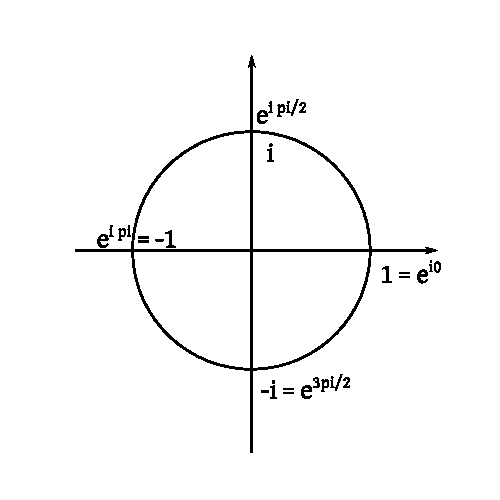
\includegraphics[width=0.5\textwidth]{img/trigonometric-periodicity.pdf}
  \end{center}
\end{figure}

\begin{rem}
  We will show: $\forall c \in (0, 2\pi)$, $\cos$ and $\sin$ are non-periodic with period $c$,
  hence $\exists x \in \mathbb R$ such that $\cos(x) \neq \cos(x + c)$.
\end{rem}

\index[English]{Periodic function}
\index[German]{\foreignlanguage{ngerman}{Periodische Funktion}}
\index[English]{Period}
\index[German]{\foreignlanguage{ngerman}{Periode}}
\begin{defi}
  \[ f: \mathbb C \to \mathbb C \qquad (f: \mathbb R \to \mathbb R) \]
  is called \emph{periodic} with period $c \in \mathbb C$ ($c \in \mathbb R$)
  if $\forall z \in \mathbb C$ it holds that
  \[ f(z + c) = f(z) \]
  \[ (\forall x \in \mathbb R: f(x + c) = f(x)) \]
  $c$ is called \emph{period of $f$}.
\end{defi}

\begin{rem}
  If $f$ is periodic with period $c \in \mathbb C$,
  then $f$ is also periodic with period $k \cdot c$ for every $k \in \mathbb Z \setminus \set{0}$.
\end{rem}

\begin{rem}
  \[ z = u + iv \]
  \[ \Re(i \cdot z) = \Re(i u - v) = -v = - \Im(z) \]
  \[ \Im(i \cdot z) = \Im(iu - v) = u = \Re(z) \]
\end{rem}

\begin{rem}
  Let $x \in \mathbb R$.
  \begin{align*}
    \cos\left(x + \frac\pi2\right)
      &= \Re(e^{i(x + \frac\pi2)}) \\
      &= \Re(e^{ix} \cdot e^{i\frac\pi2}) \\
      &= \Re(i e^{ix}) \\
      &= -\Im(e^{ix}) \\
      &= -\sin(x)
  \end{align*}

  \begin{align*}
    \sin\left(x + \frac\pi2\right)
      &= \Im\left(e^{i(x + \frac\pi2)}\right) \\
      &= \Im(ie^{ix}) \\
      &= \Re(e^{ix}) \\
      &= \cos(x)
  \end{align*}

  \begin{align*}
    \cos\left(x - \frac\pi2\right)
      &= \sin\left(x - \frac\pi2 + \frac\pi2\right) \\
      &= \sin(x)
  \end{align*}

  \begin{align*}
    \sin\left(x - \frac\pi2\right)
      &= -\cos\left(x - \frac\pi2 + \frac\pi2\right) \\
      &= -\cos(x)
  \end{align*}

  Summary:
  \begin{align*}
    \cos\left(x + \frac\pi2\right) &= -\sin(x) \\
    \sin\left(x + \frac\pi2\right) &= \cos(x) \\
    \cos\left(x - \frac\pi2\right) &= \sin(x) \\
    \sin\left(x - \frac\pi2\right) &= -\cos(x)
  \end{align*}
\end{rem}

\begin{rem}[A remark on the name \enquote{cosine}]
  \[ \sin\left(\frac\pi2 - x\right) = -\sin\left(x - \frac\pi2\right) = \cos(x) \]

  \begin{figure}[!h]
    \begin{center}
      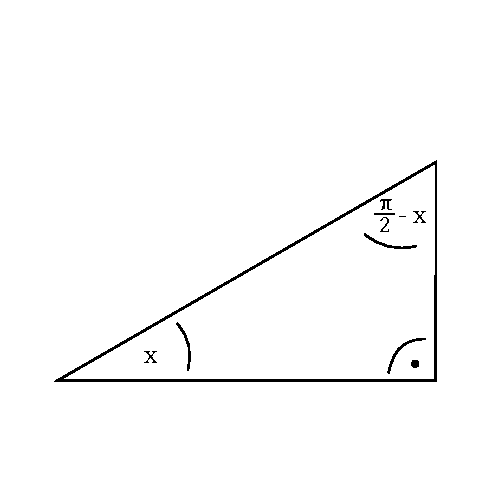
\includegraphics[width=0.4\textwidth]{img/complementary-angle.pdf}
      \caption{Complementary angle: co-sinus}
      \label{img:cosine}
    \end{center}
  \end{figure}

  The sine of the complementary angle is the co-sine of $x$ (Compare with Figure~\ref{img:cosine}).
\end{rem}

\begin{rem}
  \begin{align*}
    \cos(x + \pi) &= \Re(e^{i(x + \pi)}) \\
      &= \Re(-e^{ix}) \\
      &= -\cos(x) \\
    \sin(x + \pi) &= - \sin(x)
  \end{align*}
\end{rem}

\begin{rem}
  Let $0 < c < 2\pi$. Assume $\cos$ is periodic with period $c$.
  We know that $\cos$ has exactly one root in $[0,2]$,
  \[ \cos(x) = \cos(-x) \]
  $\cos$ has exactly two roots in $[-2,2]$, namely $\frac\pi2$ and $-\frac\pi2$.

  \begin{enumerate}
    \item Consider $c \in (0,\pi)$. Then $\cos\left(-\frac\pi2 + c\right) = \cos\left(-\frac\pi2\right) = 0$.
      \[ -\frac\pi2 + c < -\frac\pi2 + \pi = \frac\pi2 < 2 \]
      \[ -\frac\pi2 + c \geq -\frac\pi2 > -2 \]
      Therefore $\cos$ would have another root in $[-2,2]$, namely $-\frac\pi2 + c$.
      This is a contradiction.
    \item
      Consider $c \in [\pi,2\pi)$.
      $c = \pi$ is not a period because $\cos(0) = 1$ and $\cos(0 + \pi) = -1$.
      Let $\pi < c < 2\pi$.
      Then $\frac32 \pi - c < \frac32 \pi - \pi = \frac\pi2$ and $\frac32 \pi - c > \frac32 \pi - 2\pi = -\frac\pi2$.
      Hence,
      \[ \frac32 \pi - c \in \left(-\frac\pi2, \frac\pi2\right) \]
      \[ \cos\left(\frac32 \pi - c\right) = \cos\left(\frac32 \pi - c + c\right) = \cos\left(\frac32 \pi\right) = 0 \]
      $c$ would be the period.
      \[ \Rightarrow \frac32 \pi - c \text{ is a root of $\cos$ in } (-\frac\pi2, \frac\pi2) \]
      This is a contradiction.
  \end{enumerate}

  Therefore it holds that
  \[ \forall c \in (0,2\pi): \exists x \in \mathbb R: \cos(x + c) \neq \cos(x) \]
  Therefore $\cos$ is not periodic with period $c$.
  Hence $2\pi$ is indeed the smallest period of $\cos$.

  Analogously it holds for $\sin$.
\end{rem}

\begin{rem}[Roots of $\cos$]
  \[ \cos\left(\frac\pi2 + 2k\pi\right) = \cos\left(\frac\pi2\right) = 0 \qquad \forall k \in \mathbb Z \]
  \[ \cos\left(\frac32 \pi + 2k \pi\right) = \cos\left(\frac32 \pi\right) = 0 \qquad \forall k \in \mathbb Z \]
  \[ x_k = \frac\pi2 + 2k \pi = \frac{\pi}{2} \left(1 + 4k\right) \]
  \[ y_k = \frac32 \pi + 2k \pi = \frac\pi2 \left(3 + 4k\right) \]
  Hence for $z_l = \frac\pi2 \left(2l + 1\right)$ with $l \in \mathbb Z$ it holds that $\cos(z_l) = 0$.
  These are the odd multiples of $\frac\pi2$.

  \begin{align*}
    \sin(0 + 2k\pi) &= \sin(0) = 0 \\
    \sin(\pi + 2k\pi) &= \sin((2k + 1)\pi) = \sin(\pi) = 0
  \end{align*}
  \[ \Rightarrow (l\pi) = 0 \qquad \forall l \in \mathbb Z \]
\end{rem}

\subsection{Derivatives of trigonometric functions}
%
It holds that
\begin{mdframed}
  \[ \lim_{z \to 0} \frac{\sin{z}}{z} = 1 \]
\end{mdframed}
Furthermore it holds that
\begin{mdframed}
  \[ \lim_{z \to 0} \frac{1 - \cos{z}}{z} = 0 \]
\end{mdframed}

\begin{proof}
  \begin{align*}
    \frac{1 - \cos{z}}{z}
      &= \frac1z \left(1 - 1 + \frac{z^2}{2} - \frac{z^4}{4!} + \frac{z^6}{6!} - \frac{z^8}{8!} + \ldots\right) \\
      &= \frac{z}{2!} - \frac{z^3}{4!} + \frac{z^5}{6!} - \frac{z^7}{8!} + \ldots
  \end{align*}
  is convergent in $\mathbb C$ and (especially) continuous in $0$
  \[ \lim_{z \to 0} \left(\frac{z}{2!} - \frac{z^3}{4!} + \frac{z^5}{6!} - \ldots\right) = 0 \]
\end{proof}

\[
  \lim_{h\to0} \frac{\cos(x + h) - \cos(x)}{h}
\]

\meta{lecture}{11th of March 2016}{Wolfgang Ring}

Recall:
\[ \lim_{z\to0} \frac{\sin{z}}{z} = 1 \]
\[ \lim_{z\to0} \frac{1-\cos{z}}{z} = 0 \]

\begin{lemma}
  The trigonometric functions $\sin$ and $\cos$ are differentiable in $\mathbb R$
  (because they can be expressed as power series with infinite convergence radius)
  and it holds that
  \[ \cos'(x) = -\sin(x)  \qquad  \sin'(x) = \cos(x) \]
\end{lemma}
\begin{proof}
  \begin{align*}
    \lim_{h\to0} \frac{\cos(x + h) - \cos(h)}{h}
      &= \lim_{h\to0} \frac{\cos{x} \cdot \cos{h} - \sin{x} \cdot \sin{h} - \cos{x}}{h} \\
      &= \lim_{h\to0} \cos{x} \cdot \frac{\cos(h) - 1}{h} - \lim_{h\to0} \frac{\sin{x} \cdot \sin{h}}{h} \\
      &= \cos{x} \cdot \underbrace{\lim_{h\to0} \frac{\cos(h) - 1}{h}}_{=0} - \sin{x} \cdot \underbrace{\lim_{h\to0} \frac{\sin(h)}{h}}_{=1} \\
      &= -\sin(x)
  \end{align*}

  Analogously:
  \begin{align*}
    \lim_{h\to0} \frac{\sin(x + h) - \sin(h)}{h}
      &= \lim_{h\to0} \frac{\sin{x} \cdot \cos{h} + \sin{h} \cdot \cos{x} - \sin{x}}{h} \\
      &= \sin(x) \cdot \underbrace{\lim_{h\to0} \frac{\cos(h) - 1}{h}}_{=0} + \cos(x) \cdot \underbrace{\lim_{h\to0} \frac{\sin{h}}{n}}_{=1} \\
      &= \cos(x)
  \end{align*}
\end{proof}

TODO: incomplete graphics, verify text

\begin{figure}[!h]
  \begin{center}
    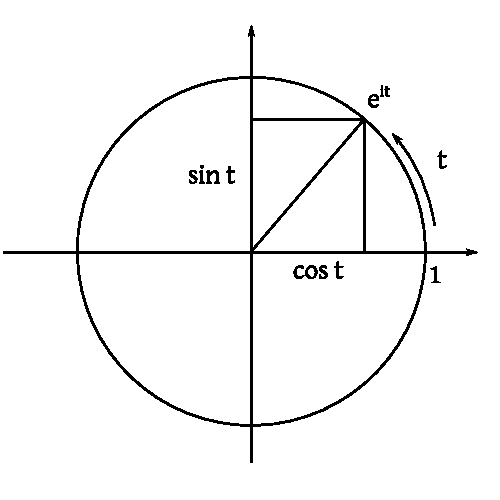
\includegraphics{img/arc-length-sincos.pdf}
    \caption{The arc length is related to $\sin$ and $\cos$}
    \label{img:arc-length}
  \end{center}
\end{figure}

Figure~\ref{img:arc-length}. We now use tools of integral calculus:

Let $I = [a,b]$ and $\gamma: I \to \mathbb R$ ($\mathbb R^2$).
\[ \gamma(t) = \begin{bmatrix} \gamma_1(t) \\ \vdots \\ \gamma_n(t) \end{bmatrix} \]
Assumption: $\gamma_1: [a,b] \to \mathbb R^n$.

\[ \gamma'(t) = \begin{bmatrix} \gamma'_1(t) \\ \vdots \\ \gamma'_n(t) \end{bmatrix} \]

TODO: graphics missing

Let $t \in [a,b]$. Then the arc length of $\gamma$ between $a$ and $t$
is given by
\[ S(t) = \int_a^t \abs{\gamma'(\tau)} \, d\tau \]

We identify $\mathbb C$ with $\mathbb R^2$:
\[ x + iy \leftrightarrow \begin{bmatrix} x \\ y \end{bmatrix} \]

\[ \gamma: t \mapsto e^{it} = \cos{t} + i \cdot \sin{t} \]
is a curve in $\mathbb C \cong \mathbb R^2$.
\[ \gamma: [0,2\pi] \to \mathbb C \]

\[ \gamma(t) = \begin{bmatrix} \cos{t} \\ \sin{t} \end{bmatrix} \]
\[ \gamma'(t) = \begin{bmatrix} -\sin{t} \\ \cos{t} \end{bmatrix} \]

\begin{figure}[!h]
  \begin{center}
    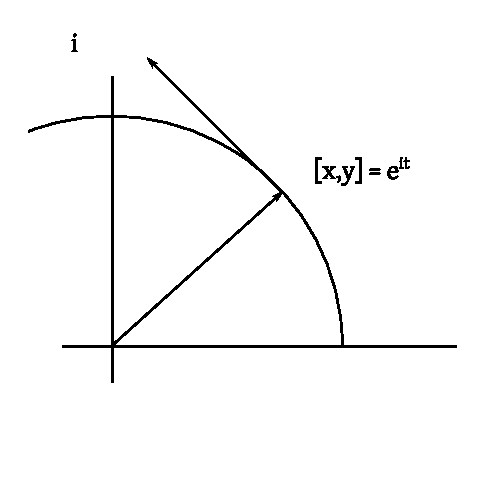
\includegraphics{img/derivative-in-r2.pdf}
    \caption{Derivative in $\mathbb R^2$}
    % TODO: incomplete
    \label{img:deriv-r2}
  \end{center}
\end{figure}

Compare with Figure~\ref{img:deriv-r2}.
\[ \abs{\gamma'(t)} = \sqrt{(-\sin(t))^2 + (\cos(t))^2} = 1 \]
\[ \int_0^t \abs{\gamma'(\tau)} \, d\tau = \int_0^t 1 \, d\tau = t \]

\section{Integration calculus}
%
Integration calculus was developed to determine areas of curves regions.
It was developed by Leibniz, Cauchy, Riemann and Lebeque. There are different
notions of integrations and it will discussed in further details in the courses
\enquote{Functional analysis} and \enquote{Measure and integration theory}.
For now, we look at the basis (as discussed by \foreignlanguage{ngerman}{Königsberger}).

\index[English]{Step function}
\index[German]{\foreignlanguage{ngerman}{Treppenfunktion}}
Let $[a,b]$ be an interval, $a,b \in \mathbb R$ with $a<b$ and $\phi: [a,b] \to \mathbb R$.
We call $\varphi$ a \emph{step function}, if $n \in \mathbb N$ and $x_0, \ldots, x_n$
exist such that
\[ x_0 = a < x_1 < x_2 < \ldots < x_n = b \]
and $\varphi|_{(x_{j-1}, x_j)} = c_j$ is constant.
The points $x_j$ define a partition of the interval $[a,b]$.

$\tau[a,b]$ defines the set of step functions of interval $[a,b]$.
The function values defining the partitions do not have any constraints and
are therefore irrelevant for further considerations (compare with Figure~\ref{img:partition-int}).

\begin{figure}[!h]
  \begin{center}
    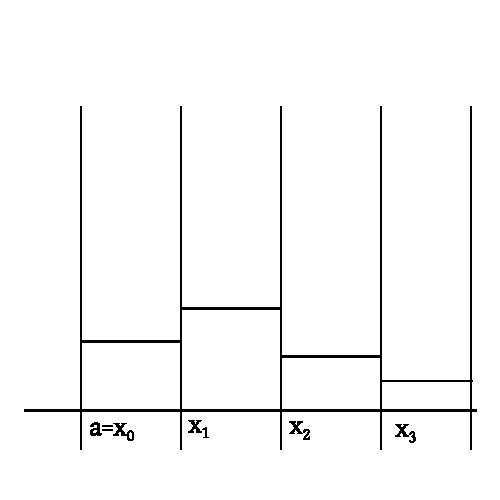
\includegraphics{img/partition-of-integral.pdf}
    \caption{Partition of an area into rectangles}
    \label{img:partition-int}
  \end{center}
\end{figure}

\index[English]{Integral}
\index[German]{\foreignlanguage{ngerman}{Integral}}
\begin{defi}
  Let $\varphi:[a,b] \to \mathbb R$ be a step function and
  $x_0 = a < x_1 < \ldots < x_n = b$ as partition of
  $[a,b]$ and let $\varphi|_{(x_{j-1}, x_j)} = c_j$
  for $j = 1,\ldots,n$.
  Then we define
  \[ \int_a^b \varphi \,dx = \sum_{j=1}^n c_j \triangle x_j \]
  where
  $\triangle x_j = x_j - x_{j-1}$ (for $j=1,\ldots,n$).
  \[ \int_a^b \varphi \, dx \text{ is called \emph{integral} of $\varphi$ over $[a,b]$} \]
\end{defi}

$\varphi$ is the step function in terms of the partition $\set{x_0,x_1,\ldots, x_5}$.

It remains to show that if $\varphi$ satisfies the definition of a step function in terms of
partition $\set{x_0,\ldots,x_n}$ and $\varphi|_{(x_{j-1}, x_j)} = c_j$
(TODO: text missing: \enquote{but \ldots})
and $\varphi$ is a step function in terms of $\set{w_0,w_1,\ldots,w_m}$
and $\varphi|_{(w_{l-1},w_l)} = c'_l$, then it holds that
\[ \sum_{j=1}^n c_j \triangle x_j = \sum_{l=1}^m c'_l \triangle w_l \]
Compare with Figure~\ref{img:step-function}.

\begin{figure}[!h]
  \begin{center}
    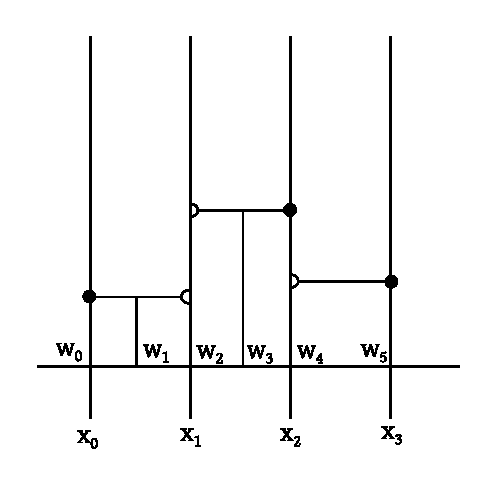
\includegraphics{img/step-function.pdf}
    \caption{Step function $\varphi$}
    \label{img:step-function}
  \end{center}
\end{figure}

% TODO: verify
\begin{proof}
  Let $Z = \set{x_0, \ldots, x_n}$ and $Z' = \set{w_0,\ldots,w_m}$.
  We define $Z'' = Z \cup Z'$ and $Z'' = \set{\alpha_0, \alpha_1, \ldots, \alpha_L}$.
  Duplicates get lost in the set.
  \[ \alpha_0 = a < \alpha_1 < \ldots < \alpha_L = b \]
  Because $Z \subseteq Z''$,
  \[ \forall x_j \exists k_j: x_j = \alpha_{k_j} \]
  Because $x_{j-1} < x_j$, it holds that $\alpha_{k_{j-1}} < \alpha_{k_j}$.
  Followingly,
  \[ k_{j-1} < k_j \]
  Let $k_{j-1} < l \leq k_j$.
  It holds that $(\alpha_{l-1}, \alpha_l) \subseteq (x_{j-1}, x_j)$,
  because $l > k_{j-1} = l-1 \geq k_{j-1} \Rightarrow \alpha_{l-1} \geq \alpha_{k_{j-1}} = x_{j-1}$
  and $l \leq k_j$.
  \[ \Rightarrow \alpha_l \leq \alpha_{k_j} = x_j \]
  So for $x \in (\alpha_{l-1}, \alpha_l) \subseteq (x_{j-1}, x_j)$ it holds that
  $\varphi(x) = c_j$.

  $k_0 = 0$ because $x_0 = \alpha_0 = a$ and $k_n = L$ because $x_n = \alpha_L = b$.
  $\forall l \in \set{0,\ldots,L}$ there exists $j \in \set{1,\ldots,n}$ such that
  $k_{j-1} \leq l \leq k_j$.

  \[ \Rightarrow \varphi|_{(\alpha_{l-1},\alpha_l)} \text{ is constant} \]

  Hence $\varphi$ is a step function in terms of the partition $\set{\alpha_0, \ldots, \alpha_L}$.

  Let $l \in \set{0,1,\ldots,L}$ and $j$ such that
  \[ k_{j-1} < l \leq k_j \Rightarrow (\alpha_{l-1},\alpha_l) \subset (x_{j-1},x_j) \]
  and $c''_l = \varphi(x)$ for $x \in (\alpha_{l-1},\alpha_l)$, then $c''_l = c_j$.

  \[ \sum_{l=1}^L c''_l \cdot \triangle \alpha_l = \sum_{j=1}^n \sum_{l=k_{j-1}+1}^{k_j} c''_l \triangle \alpha_l \]
  \[ = \sum_{j=1}^n c_j \sum_{l=k_{j-1}}^{k_j} \triangle \alpha_l \]
  \[ \sum_{l=k_{j-1} + 1}^{k_j} \triangle \alpha_l = (\alpha_{k_{j-1}+1} - \alpha_{k_{j-1}})
    + (\alpha_{k_{j-1}+2} - \alpha_{k_{j-1}+1}) + (\alpha_{k_{j-1}+3} - \alpha_{k_{j-1}+2})
  \] \[
    + \ldots + (\alpha_{k_j-1} - \alpha_{k_j-2}) + (\alpha_{k_j} - \alpha_{k_j-1})
  \]
  This is a telescoping sum. What remains is:
  \[ = \alpha_{k_j} - \alpha_{k_{j-1}} \]

  \[ x_j - x_{j-1} = \triangle x_j \]
  Analogously,
  \[ \sum_{l=1}^L c''_l \cdot \triangle \alpha_l = \sum_{k=1}^m c'_k \triangle w_k \]
  So it holds that
  \[ \sum_{j=1}^n c_j \triangle x_j = \sum_{k=1}^m c'_k \triangle w_k \]
\end{proof}

\meta{lecture}{15th of March 2016}{Wolfgang Ring}

\begin{lemma}
  Let $\varphi \in \tau[a,b]$ be a step function in terms of partition
  $a = x_0 < x_1 < \ldots < x_n = b$.
  Let $a = \alpha_0 < \alpha_1 < \ldots < \alpha_L = b$ with
  $Z = \set{x_0, \ldots, x_n} \subseteq \set{\alpha_0, \alpha_1, \ldots, \alpha_L} = z'$
  ($z'$ has more intervals than $Z'$).

  Then also $\varphi$ is step function in terms of partition $z'$.
\end{lemma}

\begin{proof}
  see above
\end{proof}

\index[English]{Linearity of integration}
\index[German]{\foreignlanguage{ngerman}{Linearität des Integral}}
\begin{lemma}
  Let $\varphi_1, \varphi_2 \in \tau[a,b]$ and $\alpha, \beta \in \mathbb C$.

  Then it holds that
  \begin{itemize}
    \item $\alpha \varphi + \beta \psi \in \tau[a,b]$ and
      \[ \int_a^b (\alpha \varphi + \beta \psi) \, dx = \alpha \int_a^b \varphi \, dx + \beta \int_a^b \psi \, dx \]
      Hence (\enquote{linearity}),
      \[ \int_a^b: \tau[a,b] \to \mathbb R \text{ is linear} \]
    \item $\abs{\varphi} \in \tau[a,b]$ and it holds that
      \[ \abs{\int_a^b \varphi \, dx} \leq \int_a^b \abs{\varphi} \, dx \leq \norm{\varphi}_\infty (b-a) \]
      Reminder: $\norm{\varphi}_\infty = \max\set{\abs{\varphi(x)}: x \in [a,b]}$ \\
      This gives \enquote{boundedness}.
    \item Let $\varphi$ and $\psi$ be real values and it holds that
      \[ \forall x \in [a,b]: \varphi(x) \leq \psi(x) \]
      Then
      TODO
      Monotonicity
  \end{itemize}
\end{lemma}
\begin{proof}
  \begin{itemize}
    \item Let $\varphi|_{(x_{k-1},x_k)} = c_k$ $\psi|_{(w_{j-1},w_j)} = d_k$
      \[ z'' = \set{\alpha_0, \alpha_1, \ldots, \alpha_L} = \set{x_0, \ldots, x_n} \cup \set{w_0, \ldots, w_m} \]
      where $\alpha_i$ is sorted ascendingly.
      $\varphi$ and $\psi$ are step functions in terms of $z''$, hence
      \[ \varphi|_{(\alpha_{i-1},\alpha_i)} = c_i' \text{ and } \psi|_{(\alpha_{i-1},\alpha_i)} = d'_i \]
      \[ \Rightarrow (\alpha \varphi + \beta \psi) |_{(\alpha_{i-1},\alpha_i)} = \alpha c_i' + \beta d_i' \text{ constant} \]
      \[ \Rightarrow \alpha \varphi + \beta \psi \in \tau[a,b] \text{ and } \int_a^b (\alpha \varphi + \beta \psi) \, dx = \sum_{i=1}^L (\alpha c'_i + \beta d'_i) \cdot \triangle \alpha_i \]
      \[ = \alpha \sum_{i=1}^L c'_i \triangle \alpha_i + \beta \sum_{i=1}^L d_i' \triangle \alpha_i \]
      \[ = \alpha \int_a^b \varphi \, dx + \beta \int_a^b \psi \, dx \]
    \item
      Let $\varphi|_{(x_{i-1},x_i)} = c_i$ ($i = 1, \ldots, n$). Then,
      \[ \abs{\varphi} |_{(x_{i-1},x_i)} = \abs{c_i} \]
      \[
        \abs{\sum_{i=1}^n c_i \triangle x_i}
        \leq \sum_{i=1}^n \abs{c_i} \cdot \underbrace{\abs{\triangle x_i}}_{x_i - x_{i-1} > 0}
        = \sum_{i=1}^n \abs{c_i} \cdot \triangle x_i = \int_a^b \abs{\varphi} \, dx
      \]
      \[
        \leq \sum_{i=1}^n \norm{\varphi}_\infty \triangle x_i
        = \norm{\varphi}_\infty \sum_{i=1}^n \triangle x_i
      \] \[
        = \norm{\varphi}_\infty \left((x_1 - x_0) + (x_2 - x_1) + \ldots + (x_{n-1} - x_{n-2}) + (x_n - x_{n-1})\right)
      \] \[
        = \norm{\varphi}_\infty (x_n - x_0) = \norm{\varphi}_\infty (b-a)
      \]
    \item
      Let $\varphi$, $\psi$ and $z''$ as in the linearity statement.
      \[
        \left.\begin{array}{rl}
          \varphi|_{(\alpha_{i-1},\alpha_i)} &= c'_i \in \mathbb R \\
          \psi|_{(\alpha_{i-1}, \alpha_i)} &= d'_i \in \mathbb R
        \end{array}\right\}
      \] \[
        \int_a^b \varphi \, dx = \sum_{i=1}^L c'_i \underbrace{\triangle \alpha_i}_{>0} \leq \sum_{i=1}^L d'_i \, dx
      \] \[
        \int_a^b \varphi \, dx
      \]
  \end{itemize}
\end{proof}
\index[English]{Characteristic function}
\index[German]{\foreignlanguage{ngerman}{Charakteristische Funktion}}
\begin{defi}
  Let $A \subseteq \mathbb R$. Then we call $\chi_A = (\mathcal 1_A): \mathbb R \to \mathbb R$ as
  \[ \chi_A(x) = \begin{cases} 1 & x \in A \\ 0 & x \not\in A \end{cases} \]
  the characteristic function of $A$. Hence $\chi_A(x)$ is $1$ if and only if $x$ is inside interval $A$.
\end{defi}
\begin{rem}
  Let $a \leq a' < b' \leq b$. Then
  \[ \chi_{(a',b')} \in \tau[a,b] \qquad \int_a^b \chi_{(a',b')} \, dx = 1 \cdot (b' - a') \]
  Every linear combination of characteristic functions is also in $\tau[a,b]$.

  On the opposite side, let $\varphi \in \tau[a,b]$ with $\varphi|_{(x_{i-1},x_i)} = c_i$
  and $\varphi(x_i) \eqqcolon r_j$ with $1 \leq i \leq n$ and $0 \leq j \leq n$.
  \[
    \Rightarrow \varphi = \sum_{i=1}^n c_i \chi_{(x_{i-1},x_i)}
    + \sum_{j=0}^n r_j \chi_{\set{x_j}}
  \]
  The step function is a linear combination of characteristic functions
  of open intervals and of characteristic functions of one-point sets.
  \[
    \int_a^b \varphi \, dx
    = \sum_{i=1}^n c_i \cdot (x_i - x_{i-1})
    = \sum_{i=1}^n c_j \int_a^b \chi_{(x_{i-1},x_i)} \, dx
  \]
\end{rem}

% TODO
\section{Regulated functions}

\index[English]{Left-sided limit}
\index[German]{\foreignlanguage{ngerman}{Linksseitiger Grenzwert}}
\index[English]{Right-sided limit}
\index[German]{\foreignlanguage{ngerman}{Rechtsseitiger Grenzwert}}
\index[English]{One-sided limit}
\index[German]{\foreignlanguage{ngerman}{Einseitiger Grenzwert}}
\begin{defi}
  Let $D \subseteq \mathbb R$. Let $x_0$ be a limit point of $D \cap (-\infty, x_0)$
  hence $\exists (z_n)_{n \in \mathbb N}$ with $z_n \in D \cap (-\infty, x_0)$,
  hence $z_n < x_0$, and $\lim_{n\to\infty} z_n = x_0$.
  Let $f: D \to \mathbb C$ be given.

  We state that $f$ has left-sided limit $y_0$ in $x_0$ if
  \[ \forall \varepsilon > 0 \exists \delta > 0: \left[x \in D \cap (-\infty, x_0) \land \abs{x - x_0} < \delta \right] \]
  \[ \Rightarrow \abs{f(x) - y_0} < \varepsilon \]

  Equivalently $\forall (z_n)_{n\in\mathbb N}$ with $z_n \in D$
  and $z_n < x_0$ and $\lim_{n\to\infty} z_n = x_0$ $\forall n \in \mathbb N$
  \[ \lim_{n\to\infty} f(x_n) = y_0 \]

  Analogously for the right-sided limes, we replace $(-\infty, x_0)$ by $(x_0, \infty)$.

  We denote: $y_0$ is left-sided limit of $f$ in $x_0$:
  \[ y_0 = \lim_{x\to x_0^-} f(x) \]
  and right-sided limit of $f$ in $x_0$:
  \[ y_0 = \lim_{x\to x_0^+} f(x) \]
\end{defi}

\index[English]{Regulated function}
\index[German]{\foreignlanguage{ngerman}{Regelfunktion}}
\begin{defi}
  Let $a,b \in \mathbb R$ and $a < b$. A function $f: [a,b] \to \mathbb C$ is called
  \emph{regulated functions} if
  \begin{itemize}
    \item $\forall x \in (a,b)$ $f$ has a left-sided and a right-sided limes in $x$
    \item $f$ has a right-sided limes in $a$
    \item $f$ has a left-sided limes in $b$
  \end{itemize}
\end{defi}

Examples for regulated functions:
\begin{itemize}
  \item Every continuous function in $[a,b]$ is a regulated function.
  \item Every step function is a regulated function. \\
    Why? Consider $x \in (x_{i-1},x_i)$. Then
    \[ \lim_{\xi\to x^+} \varphi(\xi) = c_i = \lim_{\xi \to x^-} \varphi(\xi) \]
    Let $x = x_i$ be a partitioning point.
    \[ \lim TODO \text{ and } \lim TODO \]
    So $\tau[a,b] \subseteq R[a,b]$. Compare with Figure~\ref{img:step-regulated}.
  \item
    Let $f: [a,b] \to \mathbb R$ be monotonically.
    Then it holds that
    \[ f \in R[a,b] \]
\end{itemize}

\begin{figure}[!h]
  \begin{center}
    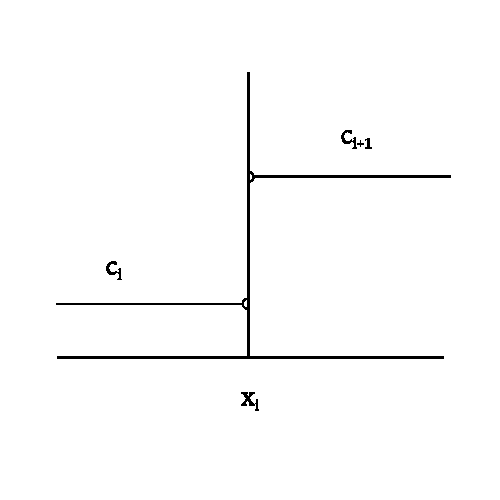
\includegraphics{img/step-functions-are-regulated-functions.pdf}
    \caption{Step functions are also regulated functions}
    \label{img:step-regulated}
  \end{center}
\end{figure}

\subsection{Approximation theorem for regulated functions}

Let $f: [a,b] \in \mathbb C$. Then it holds that $f \in R[a,b] \Leftrightarrow \forall \varepsilon > 0 \exists \varphi \in \tau[a,b]$ such that $\norm{f - \varphi}_{\infty} < \varepsilon$. Hence $\forall x \in [a,b]: \abs{f(x)}$ TODO

\[ \Leftrightarrow \underbrace{\sup\set{\abs{f(x) - \varphi(x)}: x \in [a,b]}}_{\norm{f - \varphi}_{\infty}} < \varepsilon \]

$S$ $\varepsilon_n = \frac1n \Rightarrow \exists \varphi_n \in \tau[a,b]$ such that
\[ \abs{\varphi_n(x) - f(x)} < \varepsilon \forall x \in [a,b] \]
hence $f$ is a continuous limit point of a sequence of step functions.
Hence the function sequence $(\varphi_n)_{n\in\mathbb N}$ converges continuously towards $f$.

\begin{proof}
  \begin{description}
    \item[$\Rightarrow$]
      Let $f \in R[a,b]$.
      Assume $\exists \varepsilon > 0$ fixed such that $\forall \varphi \in \tau[a,b]$
      \[ \exists x \in [a,b]: \abs{\varphi(x) - f(x)} \geq \varepsilon \]
      We build nested intervals such that the desired property $\abs{\varphi(x) - f(x)} \geq \varepsilon$
      holds on every subinterval $[a_n, b_n]$.

      Induction:
      \begin{description}
        \item[$n=0$] Let $a_0 = a$ and $b_0 = b$, hence the property holds in $[a_0, b_0]$.
        \item[$n\mapsto n+1$]
        Let $m = \frac12 (a_n + b_n)$. In $[a_n,b_n]$ the property holds.

        Then the property either holds in $[a_n,m]$ or $[m,b_n]$.
        If the property does not hold in $[a_n,m]$:
        \[ \exists \varphi_1 \in \tau[a_n,m] \text{ with } \abs{\varphi_1(\xi) - f(\xi)} < \varepsilon \qquad \forall \xi \in [a_n,m] \]
        If the property does not hold in $[m,b_n]$:
        \[ \exists \varphi_2 \in \tau[m,b_n] \text{ with } \abs{\varphi_2(\xi) - f(\xi)} < \varepsilon \qquad \forall \xi \in [m,b_n] \]
        Let
        \[
          \varphi(x) = \begin{cases}
            \varphi_1(x) & \text{ for } x \in [a_n,m] \\
            \varphi_2(x) & \text{ for } x \in [m,b_n]
          \end{cases}
        \]
        \[ \Rightarrow \varphi \in \tau[a,b] \text{ and } \abs{\varphi(\xi) - f(\xi)} < \varepsilon \qquad \forall \xi \in [a_n,b_n] \]
        So in at least one of the intervals the property holds.
        Let this interval be $[a_{n+1},b_{n+1}]$.

        $([a_n,b_n])_{n\in \mathbb N}$ are nested intervals.
        Let $\varphi \in \bigcap_{n \in \mathbb N} [a_n, b_n]$.

        \begin{description}
          \item[Case $\mathbf{\xi \in (a,b)}$]
            Let $\varepsilon$ satisfy the desired property.
            $f \in R[a,b]$, hence $f$ has left-sided limit $c_-$ in $\xi$
            and right-sided limit $c_+$. Hence $\exists \delta > 0$ such that
            \begin{itemize}
              \item $\abs{x - \xi} < \delta \land a \leq x < \xi
              \Rightarrow \abs{f(x) - c_-} < \varepsilon$
              \item $\abs{x - \xi} < \delta \land \delta < x \leq b
              \Rightarrow \abs{f(x) - c_+} < \varepsilon$
            \end{itemize}
            Choose $\delta$ sufficiently small such that
            \[ a < \xi - \delta < \xi + \delta < b \]
            Let
            \[
              \varphi(x) = \begin{cases}
                c_- & \text{ for } x \in (\xi - \delta, \xi) \\
                f(\xi) & \text{ for } x = \xi \\
                c_+ & \text{ for } x \in (\xi, \xi + \delta)
              \end{cases}
            \]
            $\varphi$ is necessarily a step function in $(\xi - \delta, \xi + \delta)$
            and it holds that $\forall x \in (\xi - \delta, \xi + \delta):
            \abs{\varphi(x) - f(x)} < \varepsilon$.

            Let $n$ be sufficiently large such that
            \[ [a_n,b_n] \subseteq (\xi - \delta, \xi + \delta) \]
            then
            \[
              \varphi|_{[a_n,b_n]} \in \tau[a_n,b_n]
              \text{ and }
              \abs{\varphi(x) - f(x)} < \varepsilon \quad \forall x \in [a_n,b_n]
            \]
            This is a contradiction to our desired property.
        \end{description}

        For $\xi = a$ or $\xi = b$ only with one-sided limit.
      \end{description}
  \end{description}
\end{proof}

\meta{lecture}{17th of March 2016}{Wolfgang Ring}

We learned: All regulated functions can be approximated with step functions.

$f \in R[a,b]$ in the proof $\Leftrightarrow$ $f$ is uniform limit of step functions.
We have prove direction $\Rightarrow$.

\begin{lemma}[Cauchy criterion for limits of functions]
  Let $f: D \subseteq \mathbb C \to \mathbb C$ and $z_0$ is a limit point
  of $D$. Then $f$ has a limit in $z_0$ if and only if $\forall \varepsilon > 0
  \exists \delta > 0: v,w \in D\setminus\set{z_0} \land \abs{v - z_0} < \delta \land
  \abs{w - z_0} < \delta \Rightarrow \abs{f(v) - f(w)} < \varepsilon$.

  If $D \subseteq \mathbb R$ and $x_0$ is limit point of $D \cap (x_0, \infty)$,
  then $f$ has a \emph{right-sided limit} in $x_0$ if and only if
  $\forall \varepsilon > 0 \exists \delta > 0: [v,w \in D \cap (x_0, \infty)
  \land \abs{v - x_0} < \delta \land \abs{w-x_0} < \delta \Rightarrow
  \abs{f(v) - f(w)} < \varepsilon]$.

  Analogously for left-sided limit.
\end{lemma}
\begin{proof}
  This proof is done only for the first point.

  \begin{description}
    \item[$\Rightarrow$] \hfill{} \\
      Assume $f$ has a limit $\eta$ in $z_0$. Choose $\delta$ such that $v,w \in D$
      with $\abs{v - z_0} < \delta$ and $\abs{w - z_0} < \delta$ implies
      that $\abs{f(v) - \eta} < \frac\varepsilon2$ and $\abs{f(w) - \eta} < \frac\varepsilon2$.
      Then $\abs{f(v) - f(w)} \leq \abs{f(v) - \eta} + \abs{\eta - f(w)}
      \leq \frac\varepsilon2 + \frac\varepsilon2 = \varepsilon$.
    \item[$\Leftarrow$] \hfill{} \\
      Assume the Cauchy criterion holds. Show: There exists $\eta \in \mathbb C$
      such that for every sequence $(w_n)_{n \in \mathbb N}$
      with $w_n \in D \setminus \set{z_0}$ with $\lim_{n\to\infty} w_n = z_0$
      it holds that $\lim_{n\to\infty} f(w_n) = \eta$.

      Let $(w_n)_{n\in\mathbb N}$ be as above. Show: $(f(w_n))_{n\in\mathbb N}$
      is a Cauchy sequence. Let $\varepsilon > 0$ be given and $\delta$ as above.
      Choose $N \in \mathbb N$ such that $n,m \geq N$
      \[ \Rightarrow \abs{w_n - z_0} < \delta \land \abs{w_m - z_0} < \delta \]
      The Cauchy criterion holds for $n,m \geq N$:
      \[ \abs{f(w_n) - f(w_m)} < \varepsilon \]
      So $(f(w_n))_{n \in \mathbb N}$ is a Cauchy sequence and (because $\mathbb C$ is complete)
      is also convergent.
      So $\exists \eta' \in \mathbb C: \lim_{n\to\infty} f(w_n) = \eta'$.

      It remains to show: $\eta'$ is unique.

      Let $(v_n)_{n\in\mathbb N}$ be another sequence with $\lim_{n\to\infty} v_n = z_0$
      and $v_n \in D \setminus \set{z_0}$. As above: $\exists \eta'' \in \mathbb C$ such that
      $\lim_{n\to\infty} f(v_n) = \eta''$.

      We construct:
      \[ (\xi_n)_{n\in\mathbb N} = (w_0, v_0, w_1, v_1, w_2, v_2, \ldots) \]
      Then it holds that $\lim_{n\to\infty} \xi_n = z_0$.

      We use the argument from above: $(f(\xi_n))_{n\in\mathbb N}$ is convergent,
      hence $\lim_{n\to\infty} f(\xi_n) = \eta$.
      Both subsequences $(f(w_n))_{n\in\mathbb N}$ and $(f(v_n))_{n\in\mathbb N}$
      must have the same limit, hence $\eta' = \eta = \eta''$.
  \end{description}
\end{proof}

\begin{proof}[Proof of approximation theorem]
  \begin{description}
    \item[$\Leftarrow$] \hfill{} \\
      Let $f = \lim_{n\to\infty} \varphi_n$ be uniform on $[a,b]$.
      Let $\varphi_n \in \tau[a,b]$ and let $x_0 \in [a,b)$.
      Show: $f$ has a right-sided limit in $x_0$.
      Let $\varepsilon > 0$ arbitrary. Choose $N \in \mathbb N$ sufficiently
      large such that
      \[
        \abs{f(x) - \varphi_N(x)} < \frac\varepsilon2
        \forall x \in [a,b]
      \]
      $\varphi_N$ is a step function (hence interval-wise constant).
      Choose $\delta > 0$ such that $\varphi_N|_{(x_0,x_0 + \delta)} = c$
      constant. Let $v,w \in (x_0, x_0 + \delta)$. Then it holds that
      \[ \abs{f(v) - f(w)} \leq \abs{f(v) - c} + \abs{c - f(w)} \]
      \[
        = \abs{f(v) - \varphi_N(v)} + \abs{f(w) - \varphi_N(w)}
        < \frac\varepsilon2 + \frac\varepsilon2 = \varepsilon
      \]
      The Cauchy criterion implies that $f$ has a right-sided limit in $x_0$.
  \end{description}
\end{proof}

\begin{cor}
  $f \in R[a,b]$ if and only if $f(x) = \sum_{j=0}^\infty \psi_j(x)$ with
  $\psi_j \in \tau[a,b]$ and the series converges uniformly in $[a,b]$.
\end{cor}
\begin{proof}
  \begin{description}
    \item[$\Leftarrow$] \hfill{} \\
      Let $\varphi_n = \sum_{j=0}^n \psi_j \in \tau[a,b]$ and $\varphi_n \to f$
      continuously in $[a,b]$. From the approximation theorem it follows that
      $f \in R[a,b]$.
    \item[$\Rightarrow$] \hfill{} \\
      Let $f \in R[a,b]$. Let $(\varphi_n)_{n \in \mathbb N}$ be a sequence of step
      functions with $\varphi_n \to f$ uniform in $[a,b]$. Let $\psi_0 = \varphi_0$.
      \[ \psi_j \coloneqq \varphi_j - \varphi_{j-1} \text{ for } j \geq 1 \]
      Then it holds that
      \[
        \sum_{j=0}^n \psi_j = \varphi_0 + (\varphi_1 - \varphi_0) +
          (\varphi_2 - \varphi_1) + \ldots + (\varphi_{n-1} - \varphi_{n-2}) +
          (\varphi_n - \varphi_{n-1})
        = \varphi_n
      \]
      and $(\varphi_n)_{n\in\mathbb N}$ converges uniform if and only if
      the series is uniformly convergent.
  \end{description}
\end{proof}

\begin{lemma}[Sidenote]
  \label{lemma-cont-func-seq}
  Let $(f_n)_{n\in\mathbb N}$ with $f_n: D \to \mathbb C$ a sequence of functions
  in $D$, let $z_0 \in D$ and $\forall n \in \mathbb N$ $f_n$ is continuous in $z_0$.
  Furthermore let $f: D \to \mathbb C$ and $f_n \to f$ is uniform in $D$.
  Then $f$ is continuous in $z_0$.
\end{lemma}
\begin{proof}
  Let $\varepsilon > 0$ arbitrary. Choose $N$ sufficiently large such that
  $\abs{f(z) - f_w(z)} < \frac\varepsilon3 \quad \forall z \in D$ (uniform convergence).
  Because $f_N$ is continuous in $z_0$, $\exists \delta > 0$ such that
  $z \in D$ and $\abs{z - z_0} < \delta$ then $\abs{f_N(z) - f_N(z_0)} < \frac\varepsilon3$.

  Then for $\abs{z - z_0} < \delta$ (with $z \in D$)
  \[
    \underbrace{\abs{f(z) - f(z_0)}}_{< \frac\varepsilon3} \leq
    \underbrace{\abs{f(z) - f_N(z)} + \abs{f_N(z) - f_N(z_0)}}_{< \frac\varepsilon3} +
    \underbrace{\abs{f_N(z_0) - f(z_0)}}_{< \frac\varepsilon3}
  \]
\end{proof}

\meta{lecture}{18th of March 2016}{Wolfgang Ring}

\begin{theorem}
  Let $f$ be a regulated function in $[a,b]$.
  Then $f$ is in at most countable infinite points of $[a,b]$ non-continuous.
\end{theorem}
\begin{proof}
  \[ f = \sum_{k=0}^\infty \psi_k \]
  where $\psi_k$ is a sequence of step functions and
  and the series is uniformly convergent.
  $\psi_k \in \tau[a,b]$.

  Let $\{x_0^k, \ldots, x_{n(k)}^k\}$ be the partition points of $\psi_k$.
  Then $\psi_k$ is continuous in $[a,b] \setminus Z_k$.
  Let $Z = \bigcup_{k=0}^\infty Z_k$ be countable.
  Let $x \in [a,b] \setminus Z$ and $\varphi_n = \sum_{k=0}^n \psi_k$.
  Then it holds that $\varphi_n \to f$ is uniform in $[a,b]$ and $\varphi_n$
  is continuous in $x$, because $x \not\in Z$.

  From Lemma~\ref{lemma-cont-func-seq} it follows that
  $f$ is continuous in $x$.
\end{proof}

\subsection{Norms and vector spaces}
%
\index[English]{Norm}
\index[German]{\foreignlanguage{ngerman}{Norm}}
\index[English]{Normed vector space}
\index[German]{\foreignlanguage{ngerman}{Normierter Vektorraum}}
\index[English]{Definity}
\index[German]{\foreignlanguage{ngerman}{Definitheit}}
\index[English]{Positive homogeneity}
\index[German]{\foreignlanguage{ngerman}{Positive Homogenität}}
\index[English]{Triangle inequality}
\index[German]{\foreignlanguage{ngerman}{Dreiecksungleichung}}
%
\begin{defi}[Normed vector spaces]
  Let $V$ be a vector space over $\mathbb C$ (or $\mathbb R$).
  A map $n: V \mapsto [0,\infty)$ is called \emph{norm} in $V$, if
  \begin{enumerate}
    \item $n(V) = 0 \Leftrightarrow V = 0$ ($V$ is null vector) \\
      \enquote{definity}
    \item $\forall \lambda \in \mathbb C$ ($\mathbb R$) $\forall v \in V: n(\lambda v) = \abs{\lambda} \cdot n(v)$
      \enquote{positive homogeneity}
    \item $\forall v,w \in V: n(v + w) \leq n(v) + n(w)$ \\
      \enquote{triangle inequality}
  \end{enumerate}
  Common notation: $\norm{v}$ for $n(v)$ (\enquote{norm of $v$}) \\
  A vector space satisfying the norm properties is called \emph{Normed vector space}
\end{defi}

\begin{ex}
  \begin{itemize}
    \item $\abs{x}$ is a norm in $\mathbb R$.
    \item $\abs{z}$ is a norm in $\mathbb C$.
  \end{itemize}
  $\norm{\vec{x}}$ is norm in $\mathbb R^n$.

  Let $D \subseteq \mathbb C$.
  \[ B(D) = \set{f: D \to \mathbb C: f \text{ limited to } D} \]
  $B(D)$ is a vector space. For $f \in B(D)$ we define:
  \[ \norm{f}_{\infty} = \sup\set{\abs{f(z)}: z \in D} \]
  \enquote{supremum norm} of $\infty$-norm of $f$ in $D$.

  It holds that $\norm{\cdot}_{\infty}$ is a norm in $B(D)$.
  \[ \norm{f}_\infty = 0 \Leftrightarrow \sup\set{\underbrace{\abs{f(z)}}_{\geq 0}: z \in D} = 0 \]
  \[ \Leftrightarrow \abs{f(z)} = 0 \quad \forall z \in D \]
  \[ \Rightarrow f = 0 \text{ in } B(D) \]
  Homogeneity:
  \begin{align*}
    \abs{\lambda \cdot f}_\infty
      &= \sup\set{\abs{\lambda f(z)}: z \in D} \\
      &= \sup\set{\abs{\lambda} \abs{f(z)}: z \in D} \\
      &= \sup\set{\abs{f(z)}: z \in D} \cdot \abs{\lambda} \\
      &= \abs{\lambda} \cdot \norm{f}_\infty
  \end{align*}
  % TODO: verify

  Triangle inequality:
  Let $f,g \in B(D)$.
  \begin{align*}
    \norm{f+g}_\infty
      &= \sup\set{\abs{f(z) + g(z)}: z \in D} \\
      &= \sup\set{\underbrace{\abs{f(z)}}_{\leq \norm{f}_\infty} + \underbrace{\abs{g(z)}}_{\leq \norm{g}_\infty}:} \\
      &\leq TODO
      &= \norm{f}_\infty + \norm{g}_\infty \\
  \end{align*}
\end{ex}

\begin{rem}
  Let $V \subseteq B(D)$ be an arbitrary subvectorspace of $B(D)$.
  So $\norm{\cdot}_\infty$ is also a norm in $V$.

  Important example:
  \[ V = \mathcal C_b(D) = \set{f: D \to \mathbb C: f \text{ is continuous and bounded in } D} \]

  Special case: $D = K$ compact in $\mathbb C$.
  Then every continuous function is also bounded.
  \begin{align*}
    \mathcal C(K) &= \set{f: K \to \mathbb C: f \text{ is continuous}} \\
      &\subseteq B(K) \qquad \text{(sub vector space)}
  \end{align*}

  Another special case: $D = [a,b] \subseteq \mathbb C$
  \[ \tau[a,b] \subseteq B([a,b]) \text{ and } \]
  \[ R[a,b] \subseteq B([a,b]) \]
\end{rem}

\begin{rem}[Further properties of the norm]
  The inverse triangle inequality holds:
  \[ \forall v,w \in V: \abs{\norm{v} - \norm{w}} \leq \norm{v - w} \]
\end{rem}
\begin{proof}
  \[ v = (v - w) + w \]
  From triangle inequality it follows that
  \[ \norm{v} \leq \norm{v - w} + \norm{w} \]
  \[ w = (w - v) + w \]
  \[ \norm{w} \leq \norm{w - v} + \norm{w} \]
  \begin{align*}
    &= \norm{(-1) \cdot (v - w)} + \norm{v} \\
    &= \abs{(-1)} \cdot \norm{v - w} + \norm{v} \\
    &= \norm{v - w} + \norm{v}
  \end{align*}
  \begin{align*}
    \text{requirement 1} &\Rightarrow \norm{v} - \norm{w} \leq \norm{v - w} \\
    \text{requirement 2} &\Rightarrow \norm{w} - \norm{v} \leq \norm{v - w} \\
    \text{requirements} &\Rightarrow  TODO
  \end{align*}
\end{proof}

\begin{defi}
  Let $V$ be a normed vector space, $(v_n)_{n\in\mathbb N}$ be a sequence of
  elements in $V$ and $v \in V$. We define $(v_n)_{n\in\mathbb N}$ is convergent
  with limit $V$ if
  \[
    \forall \varepsilon > 0 \exists N \in \mathbb N:
    \left[n \geq \mathbb N \Rightarrow \norm{V_n - V} \leq \varepsilon\right]
  \]
\end{defi}
\begin{rem}[Metric on $V$]
  \[ d(v, w) = \norm{v - w} \]
  defines a metric on $V$.
  Properties of a metric:
  \begin{enumerate}
    \item $d(v,w) \geq 0$
    \item $d(v,w) = 0 \Leftrightarrow v = w$
    \item $\norm{v - w} = 0 \Leftrightarrow v - w = 0 \Leftrightarrow v = w$
  \end{enumerate}
  Triangle inequality of metrics:
  Let $v,w,u \in V$.
  \[ d(v,u) = \norm{v - u} = \norm{v - w + w - u} \]
  \[ \leq \norm{v - w} + \norm{w - u} = d(v,w) + d(w,u) \]
  Works only if $d(v,w) = d(w,v)$ and can be simply proven:
  \[ d(v,w) = \norm{v-w} = \norm{w - v} = d(w,v) \]
\end{rem}

\index[English]{Cauchy sequence in normed vector spaces}
\index[German]{\foreignlanguage{ngerman}{Cauchyfolge in normierten Vektorräumen}}
\index[English]{Complete normed vector space}
\index[German]{\foreignlanguage{ngerman}{Vollständig normierter Vektorraum}}
\index[English]{Banach space}
\index[German]{\foreignlanguage{ngerman}{Banachraum}}
\begin{rem}
  $(V_n)_{n\in\mathbb N}$ is called \emph{Cauchy sequence in $V$} if
  \[ \forall \varepsilon > 0 \exists N \in \mathbb N: [n,m \geq N \Rightarrow \norm{v_n - v_m} < \varepsilon] \]
  $V$ is called \emph{complete normed vector space} if every Cauchy sequence in $V$
  is also a convergent sequence in $V$.

  A complete normed vector space is called \emph{Banach space}.
\end{rem}

\subsection{Integration of regulated functions}
%
\begin{theorem}
  Let $f \in \reg[a,b]$ and $\seq{\varphi_n}$ with $\varphi_n \in \tau[a,b]$ and $\varphi_n \to_{n\to\infty} f$
  uniform in $[a,b]$ ($\Leftrightarrow \norm{\varphi_n - f} \to 0$ for $n \to \infty$).

  Then we define
  \[ \int_a^b f\, dx = \lim_{n\to\infty} \int_a^b \varphi_n \, dx \]
  for the integral of $f$ in $[a,b]$.
  The right-sided limit exists for every sequence $\seq{\varphi}$ with the property above
  and is independent of the choice of the sequence $\seq{\varphi_n}$.
\end{theorem}
\begin{proof}
  Let $\seq{\varphi_n}$ such that
  \[
    \forall \varepsilon > 0 \exists N \in \mathbb N:
    [\underbrace{n \geq N \Rightarrow \abs{\varphi(x) - f(x)} < \varepsilon \forall x \in [a,b]}_{\sup\set{\abs{\varphi_n(x) - f(x)}: x \in [a,b] \leq \varepsilon}}]
  \] \[
    \Rightarrow \norm{\varphi_n - f}_\infty \leq \varepsilon
  \]
  So $\varphi_n$ converges towards $f$ in terms of $\norm{\cdot}_\infty$ in $\reg[a,b]$.

  Let $N$ be sufficiently large such that
  \[ \forall n \geq N: \norm{\varphi_n - f}_\infty < \frac\varepsilon{2(b-a)} \]
  Then it holds for $i_n = \inf_a^b \varphi_n \, dx$ and $n,m \geq N$,
  \begin{align*}
    \abs{i_n - i_m}
      &= \abs{\int_a^b \varphi_n\,dx - \int_a^b \varphi_m\,dx} \\
      &= \abs{\int_a^b (\varphi_n - \varphi_m) \, dx} \\
      &\leq \norm{\varphi_n - \varphi_m}_\infty (b-a) \\
      &= \norm{\varphi_n - f + f - \varphi_m}_\infty (b-a) \\
      &\leq (\norm{\varphi_n - f}_\infty + \norm{f - \varphi_m}_\infty) (b - a) \\
      &< \left(\frac{\varepsilon}{2(b-a)} + \frac{\varepsilon}{2(b - a)}\right)(b - a) \\
      &= \varepsilon
  \end{align*}
  So $\seq{i_n}$ is a Cauchy sequence in $\mathbb C$ and therefore convergent.
  So there exists
  \[ \lim_{n\to\infty} \int_a^b \varphi_n \, dx \]

  Let $i = \lim_{n\to\infty} \int_a^b \varphi_n \, dx$.
  Let $\seq{\psi_n}$ be another sequence of step functions with
  $\psi_n \to_{n\to\infty} f$ is uniform in $[a,b]$.
  Analogously as above:
  \[ j_n = \int_a^b \psi_n \, dx \]
  $\seq{j_n}$ is convergent and has limes $j$.

  Show that $i = j$. We again use a zip-like construction:

  \[ F = (\varphi_0, \psi_0, \varphi_1, \psi_1, \varphi_2, \ldots) \]
  $F$ is a sequence of step functions, which converge towards $f$ uniformly.
  Let $l$ be the limit of integrals of this sequence of step functions.
  Then it holds that TODO (subsequences have the same limit)
  \[ i = l = j \]
\end{proof}

\begin{theorem}[Elementary properties of the integral]
  Let $f,g \in \reg[a,b]$ and $\alpha,\beta \in \mathbb C$.
  Then it holds that
  \begin{description}
    \item[linearity]
      \[ \int_a^b (\alpha f + \beta g) \, dx = \alpha \int_a^b f \, dx + \beta \int_a^b g\, dx \]
    \item[boundedness]
      \[ \abs{\int_a^b f \, dx} \leq \int_a^b \abs{f} \, dx \leq \norm{f}_\infty (b - a) \]
    \item[monotonicity]
      Let $f,g \in \reg[a,b]$ with values in $\mathbb R$ and it holds that
      \[ f(x) \leq g(x) \qquad \forall x \in [a,b] \]
      Then it holds that
      \[ \int_a^b f\, dx \leq \int_a^b g \, dx \]
  \end{description}
\end{theorem}
\begin{proof}
  \begin{itemize}
    \item Let $\seq{\varphi_n}$ and $\seq{\psi_n}$ be sequences of step functions
      with $\varphi_n \to f$ and $\psi_n \to g$ uniform in $[a,b]$.
      Then it holds that
      \[ \alpha \varphi_n + \beta \psi_n \to_{n\to\infty} \alpha f + \beta g \]
      (proof left as exercise to the reader) \\
      uniform in $[a,b]$. So it holds that
      \begin{align*}
        \int_a^b (\alpha f + \beta g) \, dx
          &= \lim_{n\to\infty} \int_a^b (\alpha \varphi_n + \beta \psi_n) \, dx \\
          &= \alpha \lim_{n\to\infty} \int_a^b \varphi_n \, dx + \beta \lim_{n\to\infty} \int_a^b \varphi_n \, dx \\
          &= \alpha \int_a^b f \, dx + \beta \int_a^b g \, dx
      \end{align*}
    \item
      Let $\seq{\varphi_n}$ be a sequence of step functions with $\varphi_n \to_{n\to\infty} f$ continuous
      in $[a,b]$. Then also $\seq{\abs{\varphi_n}}$ is a sequence of step functions and it holds that
      \[ \abs{\varphi_n} \to_{n\to\infty} \abs{f} \text{ uniform in } [a,b] \]
      \begin{proof}
        Let $N$ be sufficiently large such that $\forall n \geq N \forall x \in [a,b]:$
        \[
          \abs{\varphi_n(x) - f(x)} < \varepsilon
          \Rightarrow \abs{\abs{\varphi_n(x)} - \abs{f(x)}} \leq \abs{\varphi_n(x) - f(x)} < \varepsilon
        \] \[
          \abs{\varphi_n} \to_{n\to\infty} \abs{f} \text{ uniform in } [a,b]
        \]
        So it holds that
        \[
          \abs{\int_a^b f \, dx}
          = \abs{\lim_{n\to\infty} \int_a^b \varphi_n \, dx}
          = \lim_{n\to\infty} \abs{\int_a^b \varphi_n \, dx}
          \leq \lim_{n\to\infty} \int_a^b \abs{\varphi_n} \, dx
          = \int_a^b \abs{f} \, dx
        \]
        Because $\abs{f - \varphi_n}_\infty \to_{n\to\infty} 0$ it follows that
        \[ \abs{\inorm{f} - \inorm{\varphi_n}} \leq \inorm{f - \varphi_n} \to 0 \]
        hence $\inorm{f} = \lim_{n\to\infty} \inorm{\varphi_n}$.
      \end{proof}
      Hence,
      \begin{align*}
        \int_a^b \abs{f} \, dx
          &= \lim_{n \to \infty} \int_a^b \abs{\varphi_n} \, dx \\
          &\leq \lim_{n\to\infty} \inorm{\varphi_n} (b - a) \\
          &= \inorm{f} (b - a)
      \end{align*}
      \begin{rem}
        We have proven that $\norm{\cdot}: V \to [0,\infty)$ is a continuous
        map, hence $v_n \to v \Rightarrow \norm{v_n} \to \norm{v}$.
      \end{rem}
  \end{itemize}
\end{proof}

\meta{lecture}{12th of April 2016}{Wolfgang Ring}

\begin{defi}
  Let $f: [a,b] \to \mathbb R$ be given.
  Let $x_0 \in [a,b)$. We claim that $f$ has a right-sided derivative $f'_+(x_0)$ in $x_0$
  if the function
  \[
    \varphi(x) = \begin{cases}
      \frac{f(x) - f(x_0)}{x - x_0} & \text{ for } x \neq x_0 \\
      0                             & \text{ for } x = x_0
    \end{cases}
  \]
  has a right-sided limit in $x_0$.
  Then $f$ is denoted with $f'_+(x_0)$.

  \[ f'_+(x_0) = \lim_{x\to x_0^+} \frac{f(x) - f(x_0)}{x - x_0} \]

  Analogously for the left-sided derivative:
  Let $x_0 \in (a,b]$. $f'_-(x_0) = \lim_{x \to x_0^-} \frac{f(x) - f(x_0)}{x - x_0}$
  if the limit exists.
\end{defi}

\begin{theorem}[Mean value theorem of calculus]
  Let $f: [a,b] \to \mathbb R$ be continuous in $[a,b]$ and $p: [a,b] \to \mathbb R$
  is a regulated function with $p(x) \geq 0 \quad \forall x \in [a,b]$.

  Then there exists $\xi \in [a,b]$ such that
  \[ \int_a^b f(x) \cdot p(x) \, dx = f(\xi) \cdot \int_a^b p(x) \, dx \]
\end{theorem}

\begin{proof}
  Let $M = \max\set{f(x): x \in [a,b]}$ and $m = \min\set{f(x): x \in [a,b]}$
  \[ m p(x) \leq f(x) \underbrace{p(x)}_{\geq 0} \leq M p(x) \qquad \forall x \in [a,b] \]
  Due to monotonicity of the integral it holds that
  \[ m \int_a^b p(x) \, dx \leq \int_a^b f(x) p(x) \, dx \leq M \int_a^b p(x) \, dx \]
  hence $\exists \eta \in [m,M]$ such that $\eta \cdot \int_a^b p(x) \, dx = \int_a^b f(x) p(x) \, dx$.
  From the Intermediate Value Theorem it follows that $\exists \xi \in [a,b]: \eta = f(\xi)$.
  \[ \Rightarrow f(\xi): \int_a^b p(x) \, dx = \int_a^b f(x) p(x) \, dx \]
\end{proof}

\begin{rem}
  Consider $p \equiv 1$.
  \[ \exists \xi \in [a,b]: \int_a^b f(x) \cdot 1 \, dx = f(\xi) \cdot \int_a^b 1 \, dx = f(\xi) \cdot (b-a) \]
  % TODO: missing
  \begin{figure}[!h]
    \begin{center}
      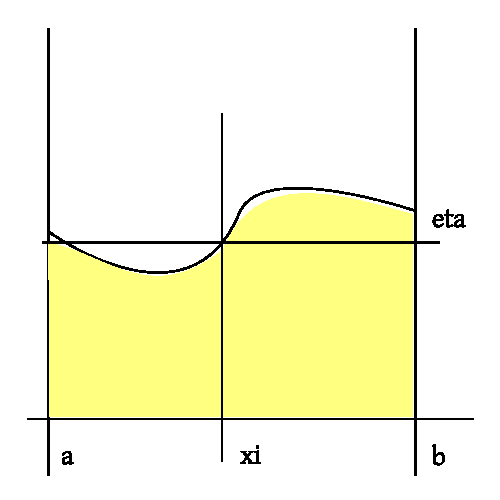
\includegraphics{img/mean_value_theorem.pdf}
      \caption{Mean value Theorem}
    \end{center}
  \end{figure}
\end{rem}

\begin{lemma}
  Let $I = [a,b]$ and $f \in R[a,b]$ and $a \leq \alpha < \beta < \gamma \leq b$ (compare with Figure~\ref{img:nl}).
  Then $f |_{[\alpha,\gamma]} \in R[\alpha,\gamma]$.

  \begin{figure}[!h]
    \begin{center}
      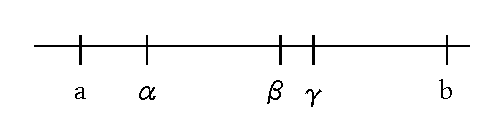
\includegraphics{img/number_line.pdf}
      \caption{Relation of $a \leq \alpha < \beta < \gamma \leq b$}
      \label{img:nl}
    \end{center}
  \end{figure}

  Furthermore it holds that
  \[ \int_{\alpha}^\beta f(x) \, dx = \int_\alpha^\beta f(x) \, dx + \int_\beta^\gamma f(x) \, dx \]
\end{lemma}

\begin{proof}
  Let $\varphi$ be a step function in $[\alpha, \gamma]$. Then $\varphi |_{[\alpha, \beta]} \in \tau[\alpha,\beta]$
  and $\varphi |_{[\beta,\gamma]} \in \tau[\beta,\gamma]$.
  Furthermore it holds (proof not given here)
  \[ \int_\alpha^\gamma \varphi \, dx = \int_\alpha^\beta \varphi \, dx = \int_\beta^\gamma \varphi \, dx \]
  For $(\varphi_n)_{n \in \mathbb N}$ a sequence of subsequences with $\varphi_n \to f$ continuous in $[\alpha,\gamma]$.
  \[ \Rightarrow \varphi_n |_{[\alpha,\beta]} \to f|_{[\alpha,\beta]} \text{ uniform in } [\alpha,\beta] \]
  analogously for $[\beta,\gamma]$.
  \[
    \int_{\alpha}^\gamma f dx
    = \lim_{n\to\infty} \int_\alpha^\gamma \varphi_n \, dx
    = \lim_{n\to\infty} \left[\int_\alpha^\beta \varphi_n \, dx + \int_\beta^\gamma \varphi_n \, dx\right]
  \] \[
    = \underbrace{\lim_{n\to\infty} \int_\alpha^\beta \varphi_n \, dx}_{=\int_\alpha^\beta f \, dx}
    + \underbrace{\lim_{n\to\infty} \int_\beta^\gamma \varphi_n \, dx}_{=\int_\beta^\gamma f \, dx}
  \]
\end{proof}

\begin{rem}
  Notation ($\alpha,\beta \in [a,b]$):
  \[ \int_\beta^\alpha f(x) \, dx = - \int_\alpha^\beta f(x) \, dx \]
  So it follows that
  \[ \int_\alpha^\alpha f(x) \, dx = - \int_\alpha^\alpha f(x) \, dx = 0 \]
  With this notation it holds that $\forall \alpha,\beta,\gamma \in I$:
  \[ \int_\alpha^\gamma f \, dx = \int_\alpha^\beta f \, dx + \int_\beta^\gamma f(x) \, dx \]
  independent of the relation of $\alpha, \beta, \gamma$ towards each other.
  For $\alpha < \beta < \gamma$ everything is fine.

  Let's also look at $\beta < \gamma < \alpha$ as an exercise.

  Then it holds that
  \[ \int_\beta^\alpha f \, dx = \int_\beta^\gamma f \, dx + \int_\gamma^\alpha f \, dx \]
  \[ - \int_\alpha^\beta f \, dx = \int_\beta^\gamma f \, dx - \int_\alpha^\gamma f \, dx \]
  \[ \Rightarrow \int_\alpha^\gamma f \, dx = \int_\alpha^\beta f \, dx + \int_\beta^\gamma f \, dx \]

  Case $\alpha = \beta$ or $\beta = \gamma$ is trivial.
\end{rem}

\index[English]{Primitive function}
\index[German]{\foreignlanguage{ngerman}{Stammfunktion}}
\index[English]{Fundamental theorem of Calculus}
\index[German]{\foreignlanguage{ngerman}{Hauptsatz der Integralrechnung}}
\begin{theorem}[Fundamental theorem of Calculus]
  Originally formulated by Isaac Barrow (1630--1677).
  Followingly popularized by Newton (1642--1727) and Leibniz (1646--1716).

  Let $f: I \to \mathbb R$ be a regulated function. $I$ is an interval and $a \in I$ is fixed.
  For $x \in I$ we define
  \[ F(x) = \int_a^x f(\xi) \, d\xi \]
  Then it holds that (two variants/characterizations)
  \begin{enumerate}
    \item $F$ is right-sided derivable and also left-sided derivable for every $x_0 \in I$
      and it holds that
      \[ F'_+(x) = f_+(x_0) = \lim_{x\to x^+_0} f(x) \qquad \text{ and } \]
      \[ F'_-(x) = f_-(x_0) = \lim_{x\to x^-_0} f(x) \]
      Especially if $f$ is continuous in $x_0$, then $F$ is differentiable in $x_0$ with
      derivative $F'(x_0) = f(x_0)$.

      We call a function with the properties of $F$ above a \emph{primitive function} of the regulated function $f$.
    \item
      Let $\Phi: I \to \mathbb R$ be an arbitrary primitive function of $f$ and
      let $a,b \in I$. Then it holds that
      \[ \int_a^b f(\xi) \, d\xi = \Phi(b) - \Phi(a) \]
  \end{enumerate}

  The first characterization claims that (informally speaking)
  the derivative for the upper limit of the integral of $f$ gives $f$.

  Let $f = \Phi'$ ($\Phi$ is our primitive function of $f$).
  The second characterization claims that the integral of a derivative of $\Phi$ gives $\Phi$.
  \[ \int_a^b \Phi' \, dx = \Phi(b) - \Phi(a) \]
\end{theorem}

\begin{proof}
  \begin{enumerate}
    \item Let $x_1, x_2 \in I$ and wlog $x_1 \leq x_2$.
      \[ \abs{F(x_1) - F(x_2)} = \abs{\int_a^{x_1} f(\xi) \, d\xi - \int_a^{x_2} f(\xi) \, d\xi} \]
      \[ = \abs{\int_a^{x_1} f(\xi) \, d\xi + \int_{x_2}^a f(\xi) \, d\xi} \]
      \[ = \abs{\int_{x_2}^{x_1} f(\xi) \, d\xi} = \abs{\int_{x_1}^{x_2} f(\xi) \, d\xi} \]
      \[ \leq \int_{x_1}^{x_2} \abs{f(\xi)} \, d\xi \leq \abs{x_2 - x_1} \cdot \norm{f}_\infty \]
      hence $F$ is Lipschitz continuous in $I$.
      So $F$ is continuous in $I$.

      One-sided limits:

      Let $\varepsilon > 0$ arbitrary and $x_0 \in I$ and $\delta$ such that $\forall x \in (x_0, x_0 + \delta)$ it holds that:
      \[ \abs{f(x) - f_+(x_0)} < \varepsilon \]
      \begin{align*}
        &\abs{\frac{F(x) - F(x_0)}{x - x_0} - f_+(x_0)} \\
        &= \frac{1}{\abs{x - x_0}} \abs{\int_a^x f(\xi) \, d\xi - \int_a^{x_0} f(\xi) \, d\xi - f_+(x_0) \cdot (x - x_0)} \\
        &= \frac{1}{\abs{x - x_0}} \abs{\int_{x_0}^x f(\xi) \, d\xi - f_+(x_0) \int_{x_0}^x 1 d\xi} \\
        &= \frac{1}{\abs{x - x_0}} \abs{\int_{x_0}^x f(\xi) \, d\xi - \int_{x_0}^x f_+(x_0) \, d\xi} \\
        &= \frac{1}{\abs{x - x_0}} \abs{\int_{x_0}^x f(\xi) - f_+(x_0) \, d\xi} \\
        &\leq \frac{1}{\abs{x - x_0}} \int_{x_0}^x \abs{f(\xi) - f_+(x_0)} \, d\xi \\
      \intertext{$\xi \in (x_0, x) \subseteq (x_0, x_0 + \delta)$}
        &< \frac{1}{\abs{x - x_0}} \cdot \varepsilon \underbrace{\int_{x_0}^x 1 \, d\xi}_{\abs{x - x_0}} \\
        &= \varepsilon \\
        &\Rightarrow F_+'(x_0) = f_+(x_0)
      \end{align*}
      Analogously $F_-'(x_0) = f_-(x_0)$.
  \end{enumerate}
\end{proof}

\meta{lecture}{14th of April 2016}{Wolfgang Ring}

\begin{theorem}[Addition: Lipschitz continuity of differentiable functions]
  Let $I = [a,b]$, $f: I \to \mathbb R$ and $f$ is continuous in $I$.
  Let $A \subseteq I$. Let $A$ be countable and $f$ is differentiable in $I \setminus A$
  and $\exists L > 0: \abs{f'(x)} \leq L \quad\forall x \in I \setminus A$.

  Then it holds that $\forall x_1, x_2 \in I$:
  \[ \abs{f(x_1) - f(x_2)} \leq L\abs{x_1 - x_2} \]
\end{theorem}
\begin{proof}
  Without loss of generality, $x_1 < x_2$. Let $\varepsilon > 0$, define
  $F_\varepsilon: I \to \mathbb R$
  \[ F_{\varepsilon}(x) = \abs{f(x) - f(x_1)} - (L + \varepsilon) (x - x_1) \]
  Show $F_\varepsilon(x_2) \leq 0$.

  Assume there is some $\varepsilon' > 0$ with $F_{\varepsilon'}(x_2) > 0$.
  It holds that
  \begin{itemize}
    \item $F_{\varepsilon'}(A) \subseteq \mathbb R$ is countable
    \item $0 = F_{\varepsilon'}(x_1) < F_{\varepsilon'}(x_2)$.
      Because $F_{\varepsilon'}$ is continuous (by Intermediate Value Theorem,
      $[0,F_{\varepsilon'}(x_2)] \subseteq F_{\varepsilon'}([x_1, x_2])$)
      and $[0, F_{\varepsilon'}(x_2)]$ contains overcountably many points,
      $F_{\varepsilon'}(A)$ is countable.
      \[ \Rightarrow \exists \gamma: 0 < \gamma < F_{\varepsilon'}(x_2) \]
      and
      \[ \gamma \in F_{\varepsilon'}([x_1, x_2] \setminus A) \]
      Let $\underbrace{F_{\varepsilon'}^{-1}(\set{y})}_{B} \cap [x_1, x_2]
      = \setdef{x \in [x_1, x_2]}{F_{\varepsilon'}(x) = y}$.

      $B$ is bounded.
      Let $c = \sup{B}$. Let $(\xi_n)_{n \in \mathbb N}$, $\xi_n \in B$ with
      $\lim_{n\to\infty} \xi_n = c$. Then it holds that $c \in [x_1, x_2]$
      and $F_{\varepsilon'}(\xi_n) = y \xRightarrow{\text{continuity of } F_{\varepsilon'}}
      \underbrace{\lim_{n\to\infty} F_{\varepsilon'}(\xi_n)}_{y} = F_{\varepsilon'}(c)$.

      Therefore $c = \max{B} = \max\set{x \in [x_1, x_2]: F_{\varepsilon'}(x) = y}$.
      Because $F_{\varepsilon'}(x_2) > y$ and $F_{\varepsilon'}(x_1) = 0 < \gamma$,
      it holds that $x_1 < c < x_2$.

      Consider $x \in (c, x_2]$ and let $\varphi(x) \coloneqq
      \frac{F_{\varepsilon'}(x) - F_{\varepsilon'}(c)}{x - c}$.
      Furthermore $F_{\varepsilon'}(x) > \gamma = F_{\varepsilon'}(c)$ for $x \in (c,x_2]$.
      Because if we define $F_{\varepsilon'}(x) < \gamma$, then (due to Intermediate Value Theorem)
      $\exists \xi \in (x, x_2)$ with $F_{\varepsilon'}(\xi) = \gamma$, so $\exists \xi \in B$
      which would be a contradiction to $c = \max{B}$.

      \begin{align*}
        \varphi(x) &= \frac{\abs{f(x) - f(x_1)} - \abs{f(c) - f(x_1)} - (L + \varepsilon')(x - x_1 - c + x_1)}{x - c} \\
          &= \frac{\abs{f(x) - f(x_1)} - \abs{f(c) - f(x_1)} - (L + \varepsilon')(x - c)}{x - c} \\
          &\overset{\text{inv. triangle ineq.}}{\leq} \frac{\abs{f(x) - f(c)}}{x - c} - (L + \varepsilon')
      \end{align*}
      Now as far as $c \not\in A$ holds, $f$ is differentiable in $c$ and it holds that $\abs{f'(c)} \leq L$,
      hence there exists an interval $(c, d)$, $d < x_2$ and $d > c$, such that
      \[ \frac{\abs{f(x) - f(c)}}{x - c} < L + \varepsilon' \]

      Because $F_{\varepsilon'}(x) > \gamma$,
      \[ \Rightarrow \varphi(x) > 0 \qquad \forall x \in (c, x_2] \]
      \[ \Rightarrow 0 < \varphi(x) \leq \abs{f(x) - f(c)}{x - c} - (L + \varepsilon') \]
      \[ \Rightarrow \abs{\frac{f(x) - f(c)}{x - c}} > L + \varepsilon' \]

      This is a contradiction to the assumption that $F_{\varepsilon'}(x_2) > 0$.
      So $F_{\varepsilon}(x_2) \leq 0 \quad \forall \varepsilon > 0$
      \[ \Rightarrow F_0(x_2) \leq 0 \Rightarrow \abs{f(x_2) - f(x_1)} \leq L - \abs{x_2 - x_1} \]
  \end{itemize}
\end{proof}

\begin{rem}
  Let $f$ be differentiable in $[a,b]$ and $\abs{f'(x)} < L \quad \forall x \in [a,b]$.
  Let $x_1, x_2 \in [a,b]$
  \[ \abs{f(x_L) - f(x_1)} = \abs{f'(\xi) \cdot (x_2 - x_1)} \leq L \abs{x_2 - x_1} \]
  by Mean Value Theorem of differential calculus.
\end{rem}

\begin{cor}
  Let $f,g: I \to \mathbb R$. $I$ as above and $f,g$ are differentiable in $I \setminus A$,
  $A$ countable and it holds that $f'(x) = g'(x) \quad \forall x \in I \setminus A$.
  There exists a constant $k$ such that
  \[ f(x) = g(x) + k \qquad \forall x \in I \]
\end{cor}
\begin{proof}
  We use the previous Theorem for
  \[ h(x) = f(x) - g(x) \]
  Then it holds that $\abs{h'(x)} = 0 = L \quad \forall x \in I \setminus A$.
  \[ \Rightarrow \abs{h(x_1) - h(x_2)} \leq 0 \cdot \abs{x_1 - x_2} \quad \forall x_1, x_2 \in I \]
  \[ \Rightarrow h(x_1) = h(x_2) \quad \forall x_1, x_2 \in I \]
  \begin{align*}
    f(x_1) - g(x_1)
      &= f(x_2) - g(x_2) \quad \forall x_1, x_2 \in I \\
      &= k \ldots \text{ constant}
  \end{align*}
  $\forall x_1 \in I$ it holds that $f(x_1) = g(x_1) + k$.
\end{proof}

\meta{lecture}{15th of April 2016}{Wolfgang Ring}

\begin{proof}[cont, 2nd part]
  We need to show: Let $f$ be a regulated function and $\Phi$ is a
  primitive function of $f$ with the following properties
  \[ \Phi'(x) = f(x) \quad \forall x \in I \text{ where f is continuous} \]
  \[ \Phi_+'(x) = \lim_{\xi\to x_+} f(x) \]
  \[ \Phi_-'(x) = \lim_{\xi\to x_-} f(x) \quad \forall x \in I \]
  Then it holds that
  \[ \int_\alpha^\beta f(x) \, dx = \Phi(\beta) - \Phi(\alpha) \]

  \begin{proof}
    For $\Phi(x) = \int_\alpha^x f(\xi) \, d\xi = F(x)$ (where $F$ is also a primitive function)
    it holds that
    \[ \int_\alpha^\beta f(\xi) \, d\xi = F(\beta) - \underbrace{F(\alpha)}_{=0} \]
    Because $\Phi$ and $F$ are both primitive functions of $f$,
    $\Phi'$ and $F'$ correspond in all continuous points,
    hence everywhere, but one countable set.

    By the uniqueness theorem, it holds that
    \[ \Phi(x) = F(x) + c \]
    \[ F(x) = \Phi(x) - c \]
    \[ \int_a^b f(\xi)\, d\xi = F(b) - F(a) = \Phi(b) - c - \Phi(a) + c = \Phi(b) - \Phi(a) \]
  \end{proof}
\end{proof}

\index[English]{Indefinite integral}
\index[German]{\foreignlanguage{ngerman}{Unbestimmtes Integral}}
\begin{rem}[Notational remark]
  Let $f$ be a regulated function. Then we denote
  \[
    \int f(x) \, dx =
    \begin{cases}
      \text{the set of all primitive function of } f & \\
      \text{an arbitrary primitive function of } f
    \end{cases}
  \]
  $\int f(x) \, dx$ is called \emph{indefinite integral}.
\end{rem}

\begin{rem}
  \[
    \int x^n \, dx = \frac{1}{n+1} x^{n+1}
    \qquad \forall n \in \mathbb R \setminus \set{-1} \forall x > 0
  \]
  If you consider all primitive functions of the indefinite integral,
  you consider a constant $c \in \mathbb R$.
  \[
    \int x^n \, dx = \frac{1}{n+1} x^{n+1} + c
    \qquad \forall n \in \mathbb R \setminus \set{-1} \forall x > 0
  \]

  Let $x > 0$: $(\ln{x})' = \frac1x$. \\
  Let $x < 0$: $(\ln{-x})' = \frac1{-x} \cdot (-1) = \frac1x$
  \[
    \int \frac 1x \, dx = \begin{cases}
      \ln(x)  & \text{ for } x > 0 \\
      \ln(-x) & \text{ for } x < 0 \\
    \end{cases}
    = \ln{\abs{x}} \qquad \text{ for } x \neq 0
  \]

  \[ \int \cos{x} \, dx = \sin{x} \]
  \[ \int \sin{x} \, dx = -\cos{x} \]
  \[ \int e^{cx} \, dx = \frac1c \cdot e^{cx} \quad (c \neq 0) \]
\end{rem}

\begin{lemma}
  Let $f_1$ and $f_2$ be regulated functions in $I = [a,b]$ and
  there exists some countable set $A$ such that
  \[ f_1(x) = f_2(x) \qquad \forall x \in I \setminus A \]
  Then it holds that
  \[
    \int f_1(x) \, dx = \int f_2(x) \, dx \text{ and } \int_a^b f_1(x) \, dx = \int_a^b f_2(x) \, dx
    \qquad \forall a,b \in I
  \]
\end{lemma}
\begin{proof}
  Let $F_1$ be a primitive function on $f_1$, $F_2$ be a primitive function of $f_2$.
  Then it holds that $F_1' = F_2'$ in $I \setminus A$.
  Due to identity theorem:
  \[ \Rightarrow F_1 = F_2 + c \Rightarrow \int f_1 \, dx = \int f_2 \, dx \]
\end{proof}

\begin{rem}
  Example of a function, which is differentiable everywhere.
  Its derivative is not a regulated function.

  Let $I = [-1,1]$ and
  \[
    f(x) = \begin{cases}
      x^2 \cdot \sin{\frac1x} & x \neq 0 \\
      0                       & x = 0
    \end{cases}
  \]
  For $x \neq 0$ it holds that
  \[ f'(x) = 2x \cos \sin{\frac1x} - \frac{x^2}{x^2} \cdot \cos{\frac1x} \]
  \[ f'(x) = 2x \sin{\frac1x} - \cos{\frac1x} \]

  \[
    f'(0)
      = \lim_{h\to0} \frac1h \left[h^2 \cdot \sin{\frac1h} - 0\right]
      = \lim_{h\to0} \underbrace{h}_{\to0} \cdot \underbrace{\sin{\frac1h}}_{\in [-1,1]}
      = 0
  \] \[
    f'(x) = \begin{cases}
      0 & \text{ for } x = 0 \\
      \underbrace{2x \sin{\frac1x} - \cos{\frac1x}}_{\text{has no one-sided limit in } x = 0} & \text{ for } x \neq 0
    \end{cases}
  \] \[
    f'_+(0) \neq \lim_{x\to 0^+} f'(x)
  \]
\end{rem}

\subsection{Integration techniques}
%
\begin{theorem}[Integration by parts (dt. \enquote{\foreignlanguage{ngerman}{partielle Integration}})]
  Let $u,v: I \to \mathbb R$ be both primitive functions of regulated functions.
  Then also $u \cdot v$ is a primitive function of a regulated function and it holds that
  \[ \int u' v \, dx = u \cdot v - \int u \cdot v' \, dx \]
  and
  \[ \int_a^b u' v \, dx = \underbrace{u(b) \cdot v(b) - u(a) \cdot v(a)}_{\eqqcolon u \cdot v |_a^b} - \int_a^b u \cdot v' \, dx \]
\end{theorem}
\begin{proof}
  $u$ is continuous and therefore a regulated function. \\
  $v$ is continuous and therefore a regulated function.

  $u'$ and $v'$ are regulated function by assumption.
  \[ \Rightarrow (u' \cdot v + u \cdot v') \in \mathcal R(I) \]
  $u \cdot v$ is differentiable in every point in which $u$ and $v$ is differentiable.
  Let $u$ be differentiable in $I \setminus A$, $v$ is differentiable in $I \setminus B$.
  \[ \Rightarrow u \cdot v \text{ is differentiable in } I \setminus \underbrace{(A \cup B)}_{\text{countable}} \]
  In $I \setminus (A \cup B)$ it holds that
  \[ (u \cdot v)'(x) = u'(x) \cdot v(x) + u(x) v'(x) \]
  Hence the function $u \cdot v$ is primitive function of the regulated function $(u' v + u v')$.
  \[ \Rightarrow \int (u' v + uv') \, dx = u \cdot v \]
  \[ \Rightarrow \int_a^b (u' v + uv') \, dx = u(b) v(b) - u(a) v(a) \]
\end{proof}

\begin{ex}
  Let $a \neq -1$ and $x > 0$.
  \[
    \int x^a \ln{x} \, dx = \begin{vmatrix}
      u' = x^a     & u = \frac1{1+a} \cdot x^{a+1} \\
      v = \ln{x}   & v' = \frac{1}{x}
    \end{vmatrix}
  \] \[
    \overset{\text{int. by parts}}{=} \frac{1}{1+a} x^{1+a} \cdot \ln{x} - \frac{1}{1+a} \int x^a \, dx
  \] \[
    = \frac{1}{1+a} x^{1+a} \ln{x} - \frac{1}{(1 + a)^2} x^{1+a}
    = \frac{1}{1+a} x^{1+a} \left[\ln{x} - \frac{1}{1 + a}\right]
  \]
\end{ex}

\begin{ex}
  \[ \int \cos^k(x) \, dx \text{ for } k = 2,3,4,\ldots \]
  \[
    \begin{vmatrix}
      u' = \cos{x} & \Rightarrow u = \sin{x} \\
      v = \cos^{k-1}(x) & v' = - (k-1) \cdot \cos^{k-2}(x) \cdot \sin(x)
    \end{vmatrix}
  \] \begin{align*}
    \int \cos^k(x) \, dx
      &= \cos^{k-1}(x) \cdot \sin(x) + \int (k-1) \cdot \cos^{k-2}(x) \cdot \underbrace{\sin^2(x)}_{1 - \cos^2(x)} \, dx \\
      &= \cos^{k-1}(x) \cdot \sin(x) + (k-1) \cdot \int \cos^{k-2}(x) \, dx - (k-1) \cdot \int \cos^k(x) \, dx
  \end{align*}
  Recognize that we have $\int \cos^k(x) \, dx$ twice in the equation (LHS and RHS, RHS with a sign).
  \[
    k \cdot \int \cos^k(x) \, dx
      = \cos^{k-1}(x) \cdot \sin(x) + (k-1) \int \cos^{k-2}(x) \, dx
  \] \[
    \int \cos^k(x) \, dx = \frac1k \cos^{k-1}(x) \sin(x) + \frac{k-1}{k} \int \cos^{k-2}(x) \, dx
  \]
  Recursion formula.

  Analogously,
  \[ \int \sin^k(x) \, dx = -\frac1k \sin^{k-1}(x) \cos(x) + \frac{k-1}{k} \int \sin^{k-2}(x) \, dx \]
  Let $c_m = \int_0^{\frac\pi2} \cos^m(x) \, dx$. Then it holds that
  \[
    c_{2n} = \frac{(2n - 1)}{2n} \cdot \frac{(2(n-1) - 1)}{2(n-1)} \cdots \frac34 \cdot \frac12 \cdot \frac\pi2
      = \left(\prod_{k=1}^n \frac{2k - 1}{2k}\right) \cdot \frac\pi2
  \] \[
    c_{2n + 1} = \left(
      \prod_{k=1}^n \frac{2k}{2k+1}
    \right)
  \]
  Proof by complete induction:
  \begin{description}
    \item[Case $n=0$]
      \[ \int_0^{\frac\pi2} \cos^{2\cdot 0} x \, dx = \int_0^{\frac\pi2} 1 \, dx = \frac\pi2 \]
      \[ \int_0^{\frac\pi2} \cos^{2\cdot 0 + 1} x \, dx = \int_0^{\frac\pi2} \cos{x} \, dx = \sin(x)|_0^{\frac\pi2} = 1 \]
      \[
        \int_0^{\frac\pi2} \cos^{2(n+1)} \, dx
          = \frac{1}{2(n+1)} \cdot \cos^{2(n+1)-1}(x) \cdot \sin(x) |_0^{\frac\pi2}
          + \frac{2(n+1) - 1}{2(n+1)} \cdot \int_0^{\frac\pi2} \cos^{2n}(x) \, dx
      \] \[
        = \frac{2n+1}{2n+2} \cdot \left(\underbrace{\prod_{k=1}^n \frac{2k-1}{2k}}_{\text{induction hypothesis}}\right) \cdot \frac\pi2
        = \left(\prod_{k=1}^{n+1} \frac{2k-1}{2k}\right) \cdot \frac\pi2
      \]
  \end{description}
\end{ex}

\begin{theorem}[Wallis product]
  (John Wallis, 1616--1703)
  \[
    \frac\pi2 = \lim_{n\to\infty} w_n
    \quad \text{with} \quad
    w_n = \prod_{k=1}^n \frac{(2k)^2}{(2k-1)(2k+1)}
    = \frac{2 \cdot 2}{1 \cdot 3} \cdot \frac{4 \cdot 4}{3 \cdot 5} \cdot \frac{6 \cdot 6}{5 \cdot 7} \ldots
  \]
\end{theorem}
\begin{proof}
  \[
    \frac\pi2 \cdot \frac{c_{2n+1}}{c_{2n}}
      = \frac\pi2 \cdot \frac{\prod_{k=1}^n \frac{2k}{2k+1}}{\prod_{k=1}^n \frac{2k-1}{2k} \cdot \frac\pi2}
      = \prod_{k=1}^n \frac{(2k)^2}{(2k + 1)(2k - 1)} = w_n
  \]
  It remains to show: $\lim_{n\to\infty} \frac{c_{2n+1}}{c_{2n}} = 1$.

  In $\left[0, \frac\pi2\right]$ it holds that $0 \leq \cos{x} \leq 1$.
  \[
    \Rightarrow \int_0^{\frac\pi2} \cos^{2n}(x) \, dx
    \geq \int_0^{\frac\pi2} \cos^{2n+1}(x) \, dx
    \geq \int_0^{\frac\pi2} \cos^{2n+2}(x) \, dx
  \] \[
    c_{2n} \geq c_{2n+1} \geq c_{2n+2}
  \] \[
    1 \geq \frac{c_{2n+1}}{c_{2n}} \geq \frac{c_{2n+2}}{c_{2n}}
    = \frac{\prod_{k=1}^{n+1} \frac{2k - 1}{2k}}{\prod_{k=1}^n \frac{2k - 1}{2k}}
    = \underbrace{\frac{2n+1}{2n+2}}_{\to 1 \text{ for } n \to \infty}
  \]
  $\Rightarrow \frac{c_{2n+1}}{c_{2n}}$ converges and limit is $1$.
  \[ \lim_{n\to\infty} \frac{\pi}2 \cdot \frac{c_{2n+1}}{c_{2n}} = \frac\pi2 = \lim_{n\to\infty} w_n \]
\end{proof}

\begin{theorem}[Substitution law]
  Let $f: I \to \mathbb R$ be a regulated function with primitive function
  $F$. Furthermore $t: [\alpha, \beta] \to I$ is continuously differentiable.
  Then $F \circ t$ is a primitive function for function $(f \circ t) \cdot t'$
  and it holds that
  \[
    \int_{\alpha}^\beta f(t(x)) \cdot t'(x) \, dx
      = \int_{t(\alpha)}^{t(\beta)} f(t) \, dt
  \]
\end{theorem}

\begin{proof}
  The right-side integral is given (according to the Fundamental Theorem) by
  \[ F(t(\beta)) - F(t(\alpha)) \]
  The left-side integral, because of
  \[ F(t(x))' = F'(t(x)) \cdot t(x) \]
  Hence $F = t$ is primitive function of the left-side integral.
  So it holds that
  \[
    \int_a^b f(t(x)) \cdot t'(x) \, dx
    = F \circ t(b) - F \circ t(a)
    = F(t(b)) - F(t(a))
  \]
\end{proof}

\begin{ex}
  \[ \int_0^1 x \sqrt{1 + x^2} \, dx = \frac12 \int_0^1 2x \sqrt{1 + x^2} \, dx \]
  \[
    \begin{vmatrix}
      t(x) = 1 + x^2    & t'(x) = 2x \\
      f(y) = \sqrt{y}   &
    \end{vmatrix}
  \] \[
    = \frac12 \int_1^2 \sqrt{x} \, dx
    = \left.\frac12 \frac{x^{\frac32}}{\frac32} \right|_1^2
    = \frac23^{\frac32} - \frac13^{\frac32}
    = \frac13 (\sqrt{8} - 1)
  \] \[
    \int_0^1 x \cdot \sqrt{1 + x^2} \, dx =
    \begin{vmatrix}
      \overbrace{y = x^2 + 1}^{\text{transform variables}}        &   \\
      \frac{dy}{dx} = 2x & \underbrace{dy = 2x \, dx}_{\text{transformation of differences}} \\
                         & x\,dx = \frac12 \, dy
    \end{vmatrix}
  \]
  Transformation of limits:
  \[ x = 0 \Leftrightarrow y = 1 \qquad x = 1 \Leftrightarrow y = 2 \]
  \[
    = \frac12 \int_1^2 \sqrt{y} \, dy
    = \left.\frac12 \frac{y^{\frac32}}{\frac32}\right|_1^2
    = \left.\frac{(x^2 + 1)^{\frac32}}{3}\right|_0^1
  \]

  Hence it is also necessary to transform the limits.
\end{ex}

\begin{ex}[Integration by parts]
  \[
    \int \ln{x} \, dx
    = \begin{vmatrix}
      v' = 1 & v = x \\
      u = \ln{x} & u' = \frac1x
    \end{vmatrix}
    = x \ln{x} - \int x \frac{1}{x} \, dx = x \ln{x} - x
  \]
\end{ex}

\index[English]{$\pi$ is irrational}
\index[German]{\foreignlanguage{ngerman}{$\pi$ is irrational}}
\begin{theorem}
  Ivan M. Niven (published in 1947, 1915--1999)

  It holds: $\pi^2$ is an irrational number. So $\pi$ is irrational.
\end{theorem}
\begin{proof}[Proof by contradiction]
  Let $\pi^2 = \frac ab \in \mathbb Q$.

  Because $\lim_{n\to\infty} \frac{a^n}{n!} = 0$ (practicals!)
  there exists $n \in \mathbb N$ such that $\pi \frac{a^n}{n!} < 1$.

  \begin{align*}
    f(x) &= \frac1{n!} x^n (1 - x)^n \\
    \intertext{is symmetrical along axis $x = \frac12$} \\
         &= \frac1{n!} \sum_{k=n}^{2n} c_k x^k \qquad \text{ with } c_k = (-1)^{k-n} \binom{n}{k-n} = \pm \binom{n}{k-n} \in \mathbb Z \\
    f^{(\mu)}(0) &= 0 \text{ for } \mu = 0,1,\ldots,n-1 \in \mathbb Z \qquad\qquad \text{ and also:} \\
    f^{(\mu)}(1) &\in \mathbb Z \text{ for } \mu = n, n+1, \ldots, 2n \\
    f^{(\mu)}(x) &= \frac1{n!} \sum_{k=0}^{2n} \underbrace{k (k-1) \ldots (k-\mu+1)}_{= \mu!} \cdot c_k \cdot x^{k-\mu} \\
    f^{(\mu)}(0) &= \frac1{n!} \mu! \left(\pm \binom{n}{\mu-n}\right) \cdot 1 \\
                 &= \frac1{n!} \mu! \frac{n!}{(\mu - n)! (n - \mu + n)!} \\
                 &= \frac{\mu!}{(\mu - n)! (2n - \mu)!} \\
                 &= \frac{(\mu-n+1) (\mu - n + 2) \ldots \mu}{1 \cdot 2 \cdot 3 \ldots (2n - \mu)} \\
                 &\in \mathbb Z
  \end{align*}
  Why does $\in \mathbb Z$ hold?
  \[ \frac{\mu!}{n!} \underbrace{\binom{n}{\mu - n}}_{\in \mathbb Z} \in \mathbb Z \qquad n \leq \mu \leq 2n \]
  \[ (n + 1) (n + 2) \ldots \nu \in \mathbb Z \]

  \[ n \leq \mu \leq 2n \]
  $f^{(\mu)}(0) \in \mathbb Z$ for $\mu \in \set{n, n+1, \ldots, 2n}$, analogously
  $f^{(\mu)}(1) \in \mathbb Z$ for $\mu \in \set{n, n+1, \ldots, 2n}$.

  \[
    F(x) = b^n \left(\pi^{2n} f(x) - \pi^{2n-2} f''(x) + \pi^{2n-4} f^{(4)} (x) + (-1)^n f^{2n}(x) \pi^0\right)
  \] \[
    F(0) \in \mathbb Z \text{ because } f^{(\mu)}(0) \in \mathbb Z \text{ for } \mu = 0,2,4,6,\ldots,2n
  \] \[
    \pi^2 = \frac ab \qquad \pi^{2n - 2l} = \frac{a^{k-l}}{b^{n-l}}
  \] \[
    b^n \cdot \pi^{2n-2l} = a^{n-l} \cdot b^l \in \mathbb Z
  \]
  Analogously for $F(1) \in \mathbb Z$.

  \[ (F'(x) \cdot \sin(\pi x) - \pi F(x) \cdot \cos(\pi x))' \]
  \[ = F''(x) \cdot \sin(\pi x) + \pi^2 \cdot F(x) \cdot \sin{\pi x} + F'(x) (\cos(\pi x) - \pi \cos{\pi x}) \]
  \[ = (F''(x) + \pi^2 F(x)) \cdot \sin(\pi x) \]
  \[ F''(x) = b^n \cdot \left(\pi^{2n} \cdot f''(x) + \pi^{2n-2} f^{(4)}(x) + \pi^{2n - 4} f^{(6)}(x) - \ldots + (-1)^n f^{(2n+2)}(x)\right) \]
  \[
    \Rightarrow F''(x) + \pi^2 \cdot F(x)
  \] \[
    = b^n \left(
      \pi^{2n} f''(x) - \pi^{2n - 2} f^{(4)}(x) + \pi^{2n - 4} f^{(6)}(x)
      + \ldots + (-1)^n f^{(2n + 2)}(x)
    \right)
  \] \[
    + b^n \left( \pi^{2n + 2} f(x) - \pi^{2n} f''(x) + \pi^{2n - 2} f^{(4)}(x)
    - \pi^{2n-4} f^{(6)}(x) + \ldots + (-1)^n \pi^2 \cdot f^{(2n)}(x) \right)
  \]
  Almost all expressions cancel each other out.
  So it holds that
  \begin{align*}
    &\left(F'(x) \cdot \sin(\pi x) - \pi F(x) \cos(\pi x)\right)' \\
    &= \pi^{2n + 2} \cdot b^n \cdot f(x) \cdot \sin(\pi x) \\
    &= \frac{a^{n+1}}{b^{n+1}} \cdot b^n \cdot f(x) \cdot \sin(\pi x) \\
    &= \frac{a^{n+1}}{b} \cdot f(x) \cdot \sin(\pi x) \\
    &= \pi^2 \cdot a^n f(x) \cdot \sin(\pi x) \\
    &= \pi \left(\pi a^n f(x) \sin(\pi x)\right) \\
    I &= \pi \int_0^1 a^n f(x) \cdot \sin(\pi x) \, dx \\
    &= \left.\frac1{\pi} \cdot \left[F'(x) \cdot \sin(\pi x) - \pi \cdot F(x) \cos(\pi x)\right]\right|_0^1 \\
    &= F(1) + F(0) \in \mathbb Z
  \end{align*}
  On the other hand it holds that
  \[ f(x) = \frac{1}{n!} \underbrace{x^{n}}_{\leq 1} (\underbrace{1 - x}_{\leq 1})^n \]
  So $0 \leq f(x) \leq \frac1{n!}$. Hence,
  \[ 0 \leq a^n f(x) \cdot \sin(\pi x) \leq \frac{a^n}{n!} < \frac{1}{\pi} \]
  So $0 < I < 1 \Rightarrow I \in \mathbb Z$. This is a contradiction to our assumption that
  $I \in \mathbb Z$.
\end{proof}

\begin{rem}
  Hence $\pi$ is not rational. So there exists no linear affine function $g(x) = ax + b$
  with $a,b \in \mathbb Z$ such that $\pi$ is root of $g$.
\end{rem}

\index[English]{Algebraic numbers}
\index[German]{\foreignlanguage{ngerman}{Algebraische numbers}}
\index[English]{Transzedente Zahlen}
\index[German]{\foreignlanguage{ngerman}{Transcedental numbers}}
\begin{rem}
  We state, $\xi \in \mathbb R$ is an \emph{algebraic} number if polynomial
  \[ P(x) = a_n x^n + a_{n-1} x^{n-1} + \ldots + a_n \]
  exists with $a_i \in \mathbb Z$ for $i = 0, \ldots, n$ and $P(\xi) = 0$.

  Algebraic numbers are a generalization of rational numbers.

  $\eta \in \mathbb R$ is called \emph{transcendental}, if $\eta$ is not algebraic.
\end{rem}

\begin{rem}
  $\pi$ is transcendental.
\end{rem}

\begin{theorem}[Integration of non-compact intervals]
  \[ \int_0^\infty e^{-x} \, dx = \lim_{c\to\infty} \int_0^c e^{-x} \, dx \]
\end{theorem}
\begin{defi}[Definition of indefinite integrals]
  Let $I$ be an interval with boundary values $a$ and $b$ with
  $- \infty \leq a < b \leq \infty$.

  Let $f$ be a regulated function in $I$. Then we define
  \begin{enumerate}
    \item if $I = [a,b)$, $\int_a^b f(x) \, dx = \lim_{\beta \to b_-} \int_a^\beta f(x) \, dx$
    \item if $I = (a,b]$, $\int_a^b f(x) \, dx = \lim_{\alpha \to a_+} \int_\alpha^a f(x) \, dx$
    \item if $I = (a,b)$, we choose $c \in I$ and $\int_a^b f(x) \, dx = \lim_{\alpha\to a_+} \int_\alpha^c f(x) \, dx + \lim_{\beta \to b_-} \int_{c}^\beta f(x) \, dx$.
  \end{enumerate}
\end{defi}

\meta{lecture}{21st of April 2016}{Wolfgang Ring}

\[ f: [a,b) \to \mathbb R \qquad b \in (-\infty, \infty] \]
\[ \int_a^b f(x) \, dx = \lim_{\beta \to b_-} \int_a^b f(x) \, dx \]

\begin{ex}[Classic examples]
  \begin{enumerate}
    \item Let $s > 1$.
      \begin{align*}
        \int_1^\infty \frac{1}{x^s} \, dx
          &= \lim \int_1^\beta x^{-s} \, dx \\
          &= \left.\frac{1}{-s+1} \cdot x^{-s+1} \right|_1^\beta \\
          &= \lim_{\beta\to\infty} \frac{1}{1 - s} \cdot \frac{1}{\beta^{s-1}} - \frac{1}{1 - s}
        \intertext{$s - 1 > 0$ and $\frac{1}{1 - s} \to 1$}
          &= \frac{1}{s - 1} \qquad \text{ so indefinite integral exists}
      \end{align*}
    \item Let $s < 1$.
      \begin{align*}
        \int_0^1 x^{-s} \, dx
          &= \lim_{\alpha\to 0_+} \int_\alpha^1 x^{-s} \, dx \\
          &= \left.\lim_{\alpha\to 0_+} \frac{1}{-s+1} x^{-s+1}\right|_{\alpha}^1 \\
          &= \frac{1}{1 - s} - \underbrace{\lim_{\alpha\to 0_+} \frac{1}{1 - s} \alpha^{1 - s}}_{= 0} \\
          &= \frac{1}{1 - s}
      \end{align*}
      Compare with Figure~\ref{img:1divs}.
    \item
      \begin{align*}
        \int_0^\infty e^{-cx} \, dx
          &= \lim_{\beta\to\infty} \int_0^\beta e^{-cx} \, dx \\
          &= \left.\lim_{\beta\to\infty} \frac{1}{-c} \cdot e^{-cx} \right|_0^\beta \\
          &= \lim_{\beta\to\infty} \left(-\frac{1}{c} \cdot e^{-c\beta}\right) + \frac1{c} \\
          &= \frac{1}{c}
      \end{align*}
    \item
      \begin{align*}
        \int_{-\infty}^{\infty} \frac{1}{1 + x^2} \, dx
          &= \lim_{\alpha\to-\infty} \int_{\alpha}^0 \frac{1}{1 + x^2} \, dx + \lim_{\beta\to0} \int_0^\beta \frac{1}{1 + x^2} \, dx \\
          &= \arctan(0) - \underbrace{\lim_{\alpha\to-\infty} \arctan(\alpha)}_{-\frac\pi2} + \underbrace{\lim_{\beta\to\infty} \arctan(\beta)}_{\frac\pi2} - \arctan(0) \\
          &= - \left(-\frac\pi2\right) + \frac\pi2 \\
          &= \pi
      \end{align*}
      % TODO: image missing (with -\frac\pi2 and shit)
  \end{enumerate}
\end{ex}

\begin{figure}[t]
  \begin{center}
    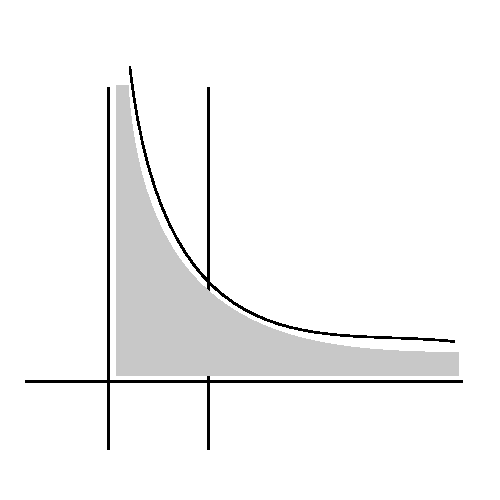
\includegraphics{img/1divsmin1.pdf}
    \caption{$\frac{1}{1 - s}$}
    \label{img:1divs}
  \end{center}
\end{figure}

\begin{rem}
  \enquote{Integral converges} means \enquote{an (indefinite) integral exists}
\end{rem}

\begin{rem}
  \[ \arctan'(x) = \frac{1}{1 + x^2} \]
  \[ \tan'(x) = \frac{\cos{x} \cdot \cos{x} - (\sin{x}) (-\sin{x})}{\cos^2{x}} = \frac{1}{\cos^2(x)} \]
  \[ \tan(x) = \frac{\sin{x}}{\cos{x}} \]
  \begin{align*}
    \arctan'(x)
      &= \frac{1}{\tan'(\arctan(x))} \\
      &= \begin{vmatrix} \arctan{x} = s \end{vmatrix} \\
      &= \left(\frac{1}{\cos^2(s)}\right)^{-1} \\
      &= \left(\frac{\cos^2(s) + \sin^2(s)}{\cos^2(s)}\right)^{-1} \\
      &= \left(1 + \left(\frac{\sin{s}}{\cos{s}}\right)^2\right)^{-1} \\
      &= \left(1 + \left[\tan(\arctan{x})\right]^2\right)^{-1} \\
      &= (1 + x^2)^{-1} \\
      &= \frac{1}{1 + x^2}
  \end{align*}
\end{rem}

\index[English]{Direct comparison test for indefinite integrals}
\index[German]{\foreignlanguage{ngerman}{Majorantenkriterium für unbestimmte Integrale}}
\begin{theorem}[Direct comparison test for indefinite integrals]
  (dt. \enquote{\foreignlanguage{ngerman}{Majorantenkriterium für uneigentliche Integrals}})
  Let $f,g$ be regulated functions in $[a,b]$ and $\abs{f(x)} \leq g(x) \quad \forall x \in [a,b)$.
  Assume $\int_a^b g(x) \, dx$ exists. Then also $\int_a^b \abs{f(x)} \, dx$ exists
  and also $\int_a^b f(x) \, dx$.
\end{theorem}

\begin{proof}
  \[ G(\beta) = \int_a^\beta g(x) \, dx \]
  We know that $\lim_{\beta\to b_-} G(\beta)$ exists.

  Cauchy criterion:
  $\forall \varepsilon > 0$ there exists a left-sided environment of $b$ such that
  for all $u,v$ in this environment it holds that
  \[ \underbrace{\abs{G(u) - G(v)}}_{\int_u^v g(x) \, dx} < \varepsilon \]
  Because $\abs{f} \leq g$ it holds that
  \[ F(\beta) = \int_a^\beta \abs{f(x)} \, dx \]
  and also that
  \[ \abs{\int_u^v \abs{f(x)} \, dx} = \abs{F(v) - F(u)} \overset{\text{monotonicity}}{\leq} \abs{\int_u^v g(x) \, dx} < \varepsilon\]
  Hence $\lim_{\beta\to b} F(\beta)$ exists because of the Cauchy criterion.
  So $\int_a^b \abs{f(x)} \, dx$ exists. Analogously for $f$ instead of $\abs{f}$.
\end{proof}

\begin{ex}
  \[ \int_0^\infty \frac{\sin{x}}{x} \, dx \text{ exists} \]
  \[
    f(x) = \begin{cases}
      \frac{\sin{x}}{x} & \text{ for } x \neq 0 \\
      1 & \text{ for } x = 0
    \end{cases}
    \text{ continuous in } 0
  \]
  \[ \int_0^1 \frac{\sin{x}}{x} \, dx = \int_0^1 f(x) \, dx \text{ exists because $f$ is continuous} \]
  \begin{align*}
    \lim_{\beta\to\infty} \int_1^\beta \frac{\sin{x}}{x} \, dx
    &= \begin{vmatrix}
      u = \frac1x & u' = -\frac1{x^2} \\
      v' = \sin{x} & v = -\cos{x}
    \end{vmatrix} \\
    &= \lim_{\beta\to\infty} \left.\frac1x \cdot (-\cos{x}) \right|_1^\beta - \int_1^\beta \frac{\cos{x}}{x^2} \, dx \\
    &= \lim_{\beta\to\infty} \left[ \underbrace{-\frac{1}{\beta} \cdot \cos{\beta}}_{\to 0} + \cos{1} - \int_1^\beta \frac{\cos{x}}{x^2} \, dx \right] \\
    &= \lim_{\beta\to\infty} \int_1^\beta \frac{\cos{x}}{x^2} \, dx
  \end{align*}
  The last expression exists, because $\frac1{x^2}$ is a majorant for $\frac{\cos(x)}{x^2}$ and $\int_1^\infty \frac{1}{x^2} \, dx$ exists.
\end{ex}

\meta{lecture}{22nd of April 2016}{Wolfgang Ring}

\[ \int_0^\infty \abs{\frac{\sin{x}}{x}} \, dx \text{ does not exist } \]
\[
  \int_{k\pi}^{(k+1)\pi} \abs{\frac{\sin{x}}{x}} \, dx
  \geq \frac{1}{(k+1) \pi} \int_{k\pi}^{(k+1)\pi} \abs{\sin{x}} \, dx
\] \[
  = \left.\frac{1}{(k+1) \pi} (\pm 1) \cdot \left(-\cos{x}\right) \right|_{k\pi}^{(k+1) \pi}
  = \frac{1}{(k+1) \pi} (\pm 1) (\pm 2)
\] \[
  = \frac{2}{(k+1)\pi}
\] \[
  \underbrace{\int_0^{(n+1)\pi} \abs{\frac{\sin{x}}{x}} \, dx}_{\text{unbounded} \Leftarrow}
    \geq \frac{2}{\pi} \cdot \underbrace{\sum_{k=0}^n \frac{1}{k+1}}_{\substack{\text{harmonic series,} \\ \text{divergent}}}
\]
In terms of the Lebesgue integral, $\int_0^\infty \frac{\sin{x}}{x} \, dx$ does not exist.

We can define new types of integration which yield new types of function which are not representable with techniques discussed so far.

\index[English]{Eulerian $\Gamma$-function}
\index[German]{\foreignlanguage{ngerman}{Eulerian $\Gamma$-function}}
\begin{ex}[The Eulerian $\Gamma$-function]
  \[ \Gamma(x) = \int_0^\infty t^{x-1} e^{-t} \, dt \text{ for } x > 0 \]
  The function variable of the $\Gamma$-function is a parameter of the integrand.
\end{ex}

The indefinite integral from above exists,
\[ \lim_{\alpha\to 0_+} \int_\alpha^1 \underbrace{t^{x-1} e^{-t}}_{>0} \, dt \text{ exists} \]
of $\int_\alpha^1 t^{x-1} e^{-t} \, dt$ is bounded in terms of $\alpha$.

\[ \int_\alpha^1 t^{x-1} \underbrace{e^{-t}}_{<1} \, dt < \underbrace{\int_\alpha^1 t^{x-1} \, dt}_{\text{converges for } x - 1 > -1} \]
hence for $x > 0$.

Right-side integral boundary:
\[ \int_1^\infty t^{x-1} e^{-t} \, dt \text{ converges?} \]

\begin{ex}[Claim]
  There exists $c > 0$ such that
  \[ t^{x-1} e^{-t} < c \cdot e^{-\frac t2} \quad \forall t \geq 1 \]

  \[ t^{x-1} \cdot e^{-\frac t2} < c \cdot e^{-\frac t2} \quad \forall t \geq 1 \]

  \begin{align*}
    \lim_{t\to\infty} \left(t^{x-1} \cdot e^{-\frac t2}\right)
    &= \begin{vmatrix} \frac t2 = s \\ t = 2s \end{vmatrix} \\
    &= \lim_{s\to\infty} (2s)^x-1 e^{-s} \\
    &\leq \lim_{s\to\infty} (2s)^{\lfloor x\rfloor + 1 - 1} \cdot e^{-s} \\
  \intertext{with $\lfloor x\rfloor \leq x < \lfloor x\rfloor + 1$}
    &= \lim_{s\to\infty} (2s)^{\lfloor x\rfloor} \cdot e^{-s} \\
    &\leq  \lim_{s\to\infty} s^{\lfloor x\rfloor + 1} \cdot e^{-s}
  \end{align*}
  because $s^{n+1} > (2s)^n$ for $s > 2^n$.

  Hence for $\varepsilon > 0$, $\exists t$ such that
  \[ \abs{t^{x-1} e^{-\frac t2}} < \varepsilon \text{ if } t > L \]
  and
  \[ \abs{t^{x-1} e^{-\frac t2}} \leq M \text{ for } t \in \underbrace{[1,L]}_{\text{compact}} \]
  $\Rightarrow$ for $t \in [1,\infty)$ it holds that
  \[
    \abs{t^{x-1} e^{-\frac t2}} \leq \max\left\{M, \varepsilon\right\} \eqqcolon c
  \]

  \[ t^{x-1} e^{-\frac t2} \leq c \]
  \[
    \int_0^\infty t^{x-1} e^{-t} \, dt
      \leq \int_0^\infty c \cdot e^{-\frac t2} \, dt
      = \left.c \cdot \left(-2 \cdot e^{-\frac t2}\right) \right|_0^\infty
      = 2c
  \]
  hence $\int_0^\infty t^{x-1} e^{-t} \, dt$ exists.

  It holds that $\Gamma(1) = 1$ because,
  \[ \int_0^\infty e^{-t} \, dt = 1 \]

  Furthermore it holds that for all $x > 0$,
  \[ \Gamma(x+1) = x \cdot \Gamma(x) \]
  \[
    \Gamma(x+1) = \int_0^\infty t^{x+1-1} e^{-t} \, dt
    = \lim_{\substack{\varepsilon \to 0 \\ R \to \infty}} \int_\varepsilon^R t^x e^{-t} \, dt
  \] \[
    = \begin{vmatrix}
      u = t^x & u' = x \cdot t^{x-1} \\
      v' = e^{-t} & v = -e^{-t}
    \end{vmatrix}
  \] \[
    = \lim_{\substack{\varepsilon \to 0 \\ R \to \infty}}\left[
      \left. -t^x e^{-t} \right|_{t=\varepsilon}^R
      + \int_\varepsilon^R x \cdot t^{x-1} \cdot e^{-t} \, dt
    \right]
  \] \[
    = \lim_{\substack{\varepsilon \to 0 \\ R \to \infty}} \left(
      \underbrace{-R^x \cdot e^{-R}}_{\to 0 \text{ for } R \to \infty} +
      \underbrace{\varepsilon^x \cdot e^{-\varepsilon}}_{\to 0 \text{ for } \varepsilon \to 0}
    \right) + x \cdot \int_0^\infty t^{x-1} e^{-t} \, dt
    = x \cdot \Gamma(x)
  \]

  So it holds that
  \begin{align*}
    T(2) &= 1 \cdot T(1) = 1 \\
    T(3) &= 2 \cdot T(2) = 2 \cdot 1 \\
    T(4) &= 4 \cdot T(3) = 3 \cdot 2 \cdot 1 \\
    T(5) &= 4 \cdot T(4) = 4 \cdot 3 \cdot 2 \cdot 1
  \end{align*}
  By complete induction we can show that
  \[ \Gamma(n+1) = n! \qquad \forall n \in \mathbb N \]
\end{ex}

\subsection{Some important inequalities}
%
\index[English]{Young's inequality}
\index[German]{\foreignlanguage{ngerman}{Young's Ungleichung}}
\begin{theorem}[Young's inequality]
  Let $f: [0, \infty) \to [0,\infty)$ be continously differentiable,
  $f(0) = 0$; $f$ is strictly monotonically increasing and unbounded
  (hence $f$ is injective because of strong monotonicity
  and surjective because of unboundedness).

  So there exists $f^{-1}: [0,\infty) \to [0,\infty)$.

  Let $a,b \geq 0$. Then it holds that
  \[
    a \cdot b \leq \int_0^a f(x) \, dx + \int_0^b f^{-1}(y) \, dy
  \]
  Equality holds if and only if,
  \[
    b = f(a) \text{ i.e. } a = f^{-1}(b)
  \]

  Compare with Figure~\ref{img:youngs-ineq}
\end{theorem}
\begin{figure}[!h]
  \begin{center}
    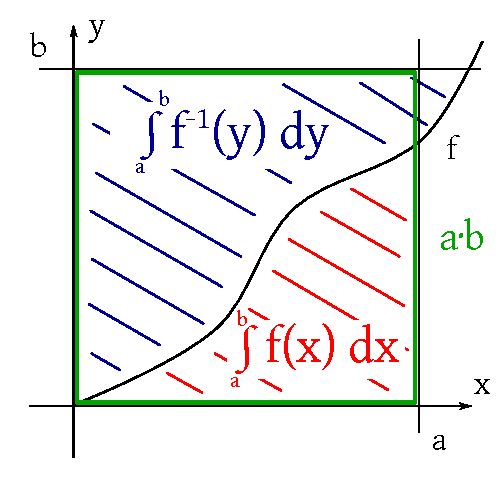
\includegraphics{img/youngs_inequality.pdf}
    \caption{Young's inequality: the blue and red areas are larger than the green area}
    \label{img:youngs-ineq}
  \end{center}
\end{figure}
\begin{proof}
  \[ \int_0^b f^{-1}(y) \, dy \overset{\text{substitution}}{=}
    \begin{vmatrix}
      y = f(x) \\
      dy = f'(x) \, dx \\
      y = 0 \Leftrightarrow x = f^{-1}(0) = 0 \\
      y = b \Leftrightarrow x = f^{-1}(b)
    \end{vmatrix}
  \]
  \begin{align*}
    &= TODO
    &= \left. f(x) x \right|_0^{f^{-1}(b)} - \int_0^{f^{-1}(b)} 1 \cdot f(x) \, dx \\
    &= f(f^{-1}(b)) \cdot f^{-1}(b) - \int_0^{f^{-1}(b)} f(x) \, dx \\
    &= b \cdot f^{-1}(b) - \int_0^{f^{-1}(b)} f(x) \, dx
  \end{align*}
  Therefore,
  \[
    \int_0^a f(x) \, dx + \int_0^b f^{-1}(y) \, dy
    = \int_0^a f(x) \, dx + \int_{f^{-1}(b)}^0 f(x) \, dx + b \cdot f^{-1}(b)
  \]

  \begin{description}
    \item[Case 1: $f^{-1}(b) = a$] ($f(a) = b$)
      \[
        \Rightarrow I = \underbrace{\int_a^b f(x) \, dx}_{=0} + b \cdot a = ab
      \]
      Proven.
    \item[Case 2: $b < f(a) \Leftrightarrow f^{-1}(b) < a$]
      $f$ is strictly monotonically increasing, hence $f(x) > f(f^{-1}(b)) = b$
      for all $x \in (f^{-1}(b), a]$.
      \[ \int_{f^{-1}(b)}^a f(x) \, dx > b \cdot \int_{f^{-1}(b)}^a 1 \, dx \]
      \[ = b \cdot \left(a - f^{-1}(b)\right) \]
      \[ I > b \left(a - f^{-1}(b)\right) + b \cdot f^{-1}(b) = a \cdot b \]
      Proven.
    \item[Case 3: $b > f(a)$]
      \[ I = \underbrace{- \int_a^{f^{-1}(b)} f(x) \, dx}_{\text{strictly mon. decreasing}} + b f^{-1}(b) \]
      For $(-f(x))$ it holds that:
      \[ > (-f(f^{-1}(b)) = -b) \]
      \[ > (-b) \left(f^{-1}(b) - a\right) + b \cdot f^{-1}(b) = a \cdot b \]
      Proven.
  \end{description}
\end{proof}
\begin{rem}
  Young's inequality also holds if $f$ has all the properties above
  but is not necessarily differentiable.
\end{rem}
\begin{theorem}[Young's inequality, special case]
  Let $A, B \geq 0$. $p,q > 1$ such that $\frac1p + \frac1q = 1$ (hence $p$ and $q$ are \enquote{conjugate exponents}).
  Then it holds that
  \[ A \cdot B \leq \frac{A^p}{p} + \frac{B^q}{q} \]
\end{theorem}
\begin{proof}
  Let $f(x) = x^{p-1}$ satisfy the requirements for Young's inequality.
  \[ f^{-1}(y) = y^{\frac{1}{p-1}} \]
  \[ \left( \frac1q = 1 - \frac1q \qquad q = \left(1 - \frac1q\right)^{-1}\right) \]
  \[ q - 1 = \left(1 - \frac1p\right)^{-1} - 1 = \left(\frac{p-1}{p}\right)^{-1} - 1 \]
  \[ = \frac{p}{p-1} - 1 = \frac{p - p + 1}{p - 1} = \frac{1}{p-1} \]
  \[ f^{-1}(y) = y^{q-1} \]
  Therefore
  \[
    A \cdot B \leq \int_0^A x^{p-1} \, dx + \int_0^B y^{q-1} \, dy
    = \left.\frac{x^p}{p}\right|_0^A + \left.\frac{y^q}{q}\right|_0^B
    = \frac{A^p}{p} + \frac{B^q}{q}
  \]
\end{proof}
\begin{rem}
  Equality holds if $A^p = B^q$. The proof is left as an exercise to the reader.
\end{rem}

\index[English]{Hölder's inequality}
\index[German]{\foreignlanguage{ngerman}{Hölder's Ungleichung}}
\begin{theorem}[Hölder's inequality]
  Let $I$ be an interval, $a, b$ are boundary values of $I$ ($a,b \in [-\infty, \infty]$).
  Let $p,q$ be conjugate exponents, hence $p,q > 1$ and $\frac1p + \frac1q = 1$.

  Let $f_1$ and $f_2$ be regulated functions in $I$ and
  \[ \int_a^b \abs{f_1(x)}^p \, dx \text{ exists and } \int_a^b \abs{f_2(x)}^q \, dx \text{ exists} \]

  Let
  \[ \norm{f_1}_p = \left(\int_a^b \abs{f_1(x)}^p \, dx\right)^{\frac1p} \]
  and
  \[ \norm{f_2}_q = \left(\int_a^b \abs{f_2(x)}^q \, dx\right)^{\frac1q} \]
  Then it holds that
  \[
    \int_a^b \abs{f_1(x) \cdot f_2(x)} \, dx \text{ exists and }
    \int_a^b \abs{f_1(x) f_2(x)} \, dx
    \leq \norm{f_1}_p \cdot \norm{f_2}_q
  \]
\end{theorem}
\begin{proof}
  Let $A = \frac{\abs{f_1(x)}}{\norm{f_1}_p}$ and $B = \frac{\abs{f_2(x)}}{\norm{f_2}_q}$.
  \[
    A \cdot b \leq \frac{A^p}{p} + \frac{B^q}{q}
  \] \[
    \overset{\text{integration}}{\Rightarrow}
    \int_a^b \frac{\abs{f_1(x)}}{\norm{f_1}_p} \cdot \frac{\abs{f_2(x)}}{\norm{f_2}_q} \, dx
    \leq \frac1p \int_a^b \frac{\abs{f_1(x)}^p}{\norm{f_1}_p^p} \, dx
    + \frac1q \int_a^b \frac{\abs{f_2(x)}^q}{\norm{f_2}_q^q} \, dx
  \] \[
    \Rightarrow \frac{1}{\norm{f_1}_p \norm{f_2}_q} \cdot
    \int_a^b \abs{f_1(x) \cdot f_2(x)} \, dx
  \] \[
    \leq \frac{1}{p} \frac{1}{\norm{f_1}_p^p} \underbrace{\int_a^b \abs{f_1(x)}^p}_{\norm{f_1}_p^q} \, dx
    + \frac1q \frac1{\norm{f_2}_q^q} \underbrace{\int_a^b \abs{f_2(x)}^q}_{\norm{f_2}_q^q} \, dx
  \] \[
    = \frac1p + \frac1q = 1
  \] \[
    = \underbrace{\int_a^b \abs{f_1(x) \cdot f_2(x)} \, dx}_{\text{exists}}
    \leq \norm{f_1}_p \cdot \norm{f_2}_q
  \]
\end{proof}

\meta{lecture}{28th of April 2016}{Wolfgang Ring}

\begin{ex}[Special case $p = q = 2$]
  Let $p = q = 2$. $\frac12 + \frac12 = 1$ holds.
  \[
    \int_a^b \abs{f_1(x) \cdot f_2(x)} \, dx
    \leq \left(\int_a^b \abs{f_1(x)}^2 \, dx\right)^{\frac12}
    \cdot \left(\int_a^b \abs{f_2(x)}^2 \, dx\right)^{\frac12}
  \] \[
    \int_a^b \abs{f_1(x) \cdot f_2(x)} \, dx \geq \abs{\int_a^b f_1(x) \cdot f_2(x) \, dx}
  \]
  $f_1$ and $f_2$ such that $\norm{f_i}_2 < \infty$ for $i = 1,2$,
  then
  \[ \fun{f_1, f_2} = \int_a^b f_1(x) \cdot f_2(x) \, dx \]
  is a scalar (= inner) product in the vector space of functions
  with norm:
  \[
    \norm{f} = (\fun{f, f})^{\frac12} = \norm{f}_2
  \]
\end{ex}

\index[English]{Cauchy-Schwarz inequality}
\index[German]{\foreignlanguage{ngerman}{Cauchy-Schwarz Ungleichung}}
The resulting inequality is named \enquote{Cauchy-Schwarz inequality}
\[
  \abs{\fun{f_1, f_2}} \leq \norm{f_1}_2 \cdot \norm{f_2}_2
\]

\subsection{Elementwise integration of series}
%
\begin{lemma}
  Let $f_n \in R(I)$ with $I$ as interval, $f_n$ converges uniformly to $f$ in $I$.
  Then also $f$ is a regulated function and
  \[ \int_a^b f(x) \, dx = \lim_{n\to\infty} \int_a^b f_n(x) \, dx \]
\end{lemma}
\begin{proof}
  We know $f$ is a regulated function if and only if $f$ can be uniformly
  approximated using a step function.

  Let $\varepsilon > 0$ be arbitrary.
  Because $f$ is the uniform limit of $f_n$, there exists $n \in \mathbb N$
  such that $\inorm{f - f_N} < \frac\varepsilon2$. Because $f_N$ is a regulated
  function, there exists $\varphi \in \tau(I)$ with
  \[
    \inorm{f_N - \varphi} < \frac\varepsilon2 \Rightarrow
    \inorm{f - \varphi} \leq \inorm{f - f_N} + \inorm{f_N - \varphi}
    < \frac\varepsilon2 + \frac\varepsilon2 = \varepsilon
  \]
  Hence $f$ is a regulated function.
  Choose $N$ such that $\forall n \geq N$:
  \[ \inorm{f - f_n} < \frac\varepsilon{b - a} \]
  Then it holds that
  \begin{align*}
    \abs{\int_a^b f_n(x) \, dx - \int_a^b f(x) \, dx}
      &\leq \int_a^b \abs{f_n(x) - f(x)} \, dx \\
      &\leq \int_a^b \underbrace{\inorm{f_n - f}}_{< \frac\varepsilon{b - a}} \, dx \\
      &< \frac\varepsilon{b - a} \cdot (b - a) \\
      &= \varepsilon
  \end{align*}
\end{proof}

\begin{ex}[Application]
  Let $f(x) = \sum_{n=0}^\infty a_k x^k$ is a power series.
  Let $\rho_f$ be a convergence radius of $f$ and $0 < r < \rho_f$.
  Then it holds that
  \[ f_n(x) = \sum_{k=0}^n a_k x^k \text{ converges uniformly to $f$ in $[-r,r]$} \]
  \[ f_n \in R([-r,r]) \]
  \[
    \Rightarrow
    \int_{-r}^r f(x) \, dx
    = \lim_{n\to\infty} \int_{-r}^r f_n(x) \, dx
  \]
  The integral is determined by elementwise integration
  \[ \int_{-r}^r a_k x^k \, dx = \left. a_k \frac{x^{k+1}}{k+1} \right|_{-r}^r \]
  Analogously for integration over any compact interval $[a,b] \subset (-\rho_f, \rho_f)$
  i.e. for the indefinite integration. Hence,
  \[ \sum_{k=0}^\infty a_k \frac{x^{k+1}}{n+1} + c \]
  is primitive function of $f$ uniformly convergent on every interval
  $[-r,r] \subseteq (-\rho_f, \rho_f)$.
\end{ex}

\begin{ex}
  \[ F: \mathbb R \to \left(-\frac\pi2, \frac\pi2\right) \qquad F(x) = \arctan(x) \]
  \[
    F'(x) = f(x) = \frac{1}{1 + x^2}
    = \sum_{k=0}^\infty \left(-(x^2)\right)^k = \sum_{k=0}^\infty (-1)^k x^{2k}
    \qquad \forall x \in (-1, 1)
  \]

  Elementwise integration:
  \[ F(x) = \arctan(x) = \sum_{k=0}^\infty (-1)^k \frac{x^{2k+1}}{2k + 1} + c \]
  \[ \arctan(0) = 0 = c \]
  Hence,
  \[ \arctan(x) = \sum_{k=0}^\infty (-1)^k \frac{x^{2k+1}}{2k + 1} \quad \text{ in } (-1, 1) \]
  Compare with Figure~\ref{img:arctan-approx}
\end{ex}

\begin{figure}[!h]
  \begin{center}
    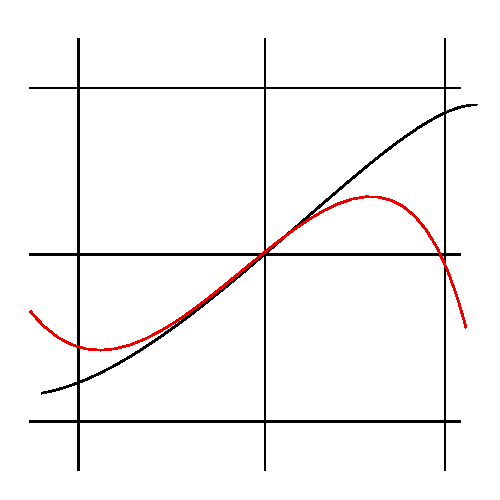
\includegraphics{img/approximation_of_arctan.pdf}
    \caption{Approximation of $\arctan(x)$}
    \label{img:arctan-approx}
  \end{center}
\end{figure}

\section{Taylor polynomials and Taylor series}
%
\begin{theorem}
  Approximation of a function with polynomials or representation
  of a function using a power series.
  \[
    \mathcal C^n((a,b))
    = \setdef{f: (a,b) \to \mathbb R}{f \text{ differentiable $n$ times in } (a,b)}
  \]
  Hence $f^{(k)}: (a,b) \to \mathbb R$ is continuous for $k = 0, 1, \ldots, n$.
  Choose $x_0 \in (a,b)$.
  Find a polynomial $T_f^a(x)$ of degree $n$ such that
  \[ \left(T_f^a\right)^{(k)}(x_0) = f^{(k)}(x_0) \]
  It holds that $T_f^a$ can be determined uniquely as
  \[ T_f^a(x) = \sum_{k=0}^n \frac{f^{(k)}(x_0)}{k!} (x - x_0)^k \]
  Taylor polynomial of $n$-th order of $f$ in point $x_0$.
\end{theorem}

\meta{lecture}{29th of April 2016}{Kniely Michael}

\begin{defi}[Additional remark to Taylor polynomials]
  Let $P(x) \coloneqq \sum_{k=0}^n a_k x^k$, $a_n \neq 0$. Let $k \in \set{1, \ldots, n}$.
  \begin{enumerate}
    \item $x_0$ is called $k$-th root of $P$ iff $P(x) = (x - x_0)^k Q(x)$ with $Q(x_0) \neq 0$.
    \item It holds that $x_0$ is a $k$-th  root of $P$ iff
      \[ \forall j \in \set{0,\ldots,k-1}: P^{(j)}(x_0) = 0 \land P^{(k)}(x_0) \neq 0 \]
  \end{enumerate}
\end{defi}
\begin{proof}[Complete induction over $k$]
  \begin{description}
    \item[$\mathbf{k=1}$] \hfill{} \\
      $\Rightarrow$: Let $x_0$ be 1st root of $P$.
        \[ P(x) = (x - x_0) Q(x) \Rightarrow P^{(0)}(x_0) = 0 \land P^{(1)}(x_0) = Q(x_0) \neq 0. \]
      $\Leftarrow$: Let $P^{(0)}(x_0) = 0$.
        \[ P^{(1)}(y_0) \neq 0 \]
        Division with remainder $\Rightarrow$
        \[ P(x) = (x - x_0) Q(x) + R(x) \text{ with } \deg(R) < \deg(x - x_0) = 1 \]
        with $R$ constant.
        \[ 0 = P(y_0) = R \Rightarrow P(x) = (x - x_0) Q(x) \]
        \[
          x \neq x_0 \Rightarrow Q(x) = \frac{P(x)}{x - x_0}
          = \frac{P(x) - P(x_0)}{x - x_0}
          \Rightarrow Q(x_0)
        \] \[
          \overset{\text{Q continuous}}{=}
          \lim_{x\to x_0} Q(x) = \lim_{x \to x_0} \frac{P(x) - P(x_0)}{x - x_0}
          = P^{(1)}(x_0) \neq 0
        \]
    \item[$\mathbf{k\geq 2, k-1 \to k}$]
      $\Rightarrow$. Let $x_0$ be the k-th root of $P$.
      Hence $P(x) = (x - x_0)^k Q(x)$ with $Q(x_0) \neq 0$.
      Let $\tilde{P}(x) \coloneqq (x - x_0)^{k-1} Q(x)$.
      $x_0$ is $(k-1)$-th root of $\tilde{P}$.
      \[
        \xRightarrow{\text{ind. hypo.}}
        \tilde{P}^{(j)}(x_0) = 0
        \land \tilde{P}^{(k-1)}(x_0) \neq 0
        \quad \forall j \in \set{0,\ldots,k-2}
      \] \[
        P(x) = (x - x_0) \tilde{P}(x) \Rightarrow
        P^{(j)}(x) = (x - x_0) \tilde{P}^{(j)}(x) + j \tilde{P}^{(j-1)}(x)
      \]
      We prove the last statement using complete induction:
      \begin{proof}
        \begin{description}
          \item[$j=0$]
            Follows immediately.
          \item[$j \geq 0, j \to j+1$]
            \[ P^{(j+1)}(x) = \left(P^{(j)}\right)'(x) \]
            \[
              = \tilde{P}^{(j)}(x) + \tilde{P}^{(j+1)}(x) (x - x_0)
            \] \[
              + j \tilde{P}^{(j)}(x)
              = (x - x_0) \tilde{P}^{(j+1)}(x) + (j+1)P^{j}(x).
            \] \[
              P^{(j)}(x_0) = j \tilde{P}^{(j-1)}(x_0)
            \] \[
              \begin{cases}
                = 0 & j = 0,\ldots,k-1 \\
                \neq 0 & j = k
              \end{cases}
            \]
        \end{description}
      \end{proof}

      We then prove the second part: $\Leftarrow$.

      Let $P^{(j)}(x_0) = 0$ for $j \in \set{0,\ldots,k-1}$, $P^{(k)}(x_0) \neq 0$.
      It holds that $P(y_0) = 0$ because of $P^{(0)}(x_0) = 0$.
      Like above: $P(x) = (x - x_0) \tilde{P}(x)$ and
      \[ P^{(j)}(x) = (x - x_0) \tilde{P}^{(j)}(x) + j \tilde{P}^{(j-1)}(x). \]
      \[ j \in \set{1,\ldots,k-1} \Rightarrow 0 = P^{(j)}(x_0) = TODO \]
      \[ \Rightarrow \forall l \in \set{0,\ldots,k-2}: \tilde{P}^{(l)}(x_0) = 0 \]
      TODO

      \[ 0 \neq P^{(k)}(x_0) = k \tilde{P}^{(k-1)}(x_0) \Rightarrow \tilde{P}^{)k-1}(x_0) \neq 0 \]

      induction hypothesis $\Rightarrow$
      \[ \tilde{P}(x) = (x - x_0)^{k-1} Q(x) \text{ with } Q(x_0) \neq 0 \]
      \[ \Rightarrow P(x) = (x - x_0) \tilde{P}(x) = (x - x_0)^k Q(x). \]
  \end{description}
\end{proof}

\index[English]{Taylor polynomial}
\index[German]{\foreignlanguage{ngerman}{Taylorpolynom}}
\begin{theorem}
  Let $f$ in $\mathbb C^n((a,b))$ with $n \in \mathbb N$.
  Let $a,b \in [-\infty, \infty]$, $x_0 \in (a,b)$.
  Find a polynomial $T$ of degree $n$ such property
  \begin{align}
    \forall k \in \set{0,\ldots,n}: T^{(k)}(x_0) = f^{(k)}(x_0).
    \label{taypoly}
  \end{align}
  Claim:
  \[ T_f^n(x) \equiv T_f^n(x; x_0) \coloneqq \sum_{k=0}^n \frac{f^{(k)}(x_0)}{k!} (x - x_0)^k \]
  where $x_0$ is the base point, is the only polynmial of degree $n$, which satisfies
  property~\ref{taypoly}.

  $T_f^n$ is called \emph{Taylor polynomial} of $n$-th degree of $f$ in $x_0$.
\end{theorem}
\begin{proof}
  Let $k \in \set{0,\ldots,n}$.
  \[ (T_g^n)^{(k)}(x) = \sum_{j=k}^n \frac{f^{(j)}(x_0)}{j!} j (j-1) \cdot \ldots \cdot (j - (k-1))(x - x_0)^{j-k} \]
  \[
    \left(T_f^n\right)^{(k)} (x_0)
    = \frac{f^{(k)}(x_0)}{k!} \underbrace{\left(k \cdot \ldots \cdot (k - (k-1))\right)}_{= k!}
    = f^{(k)}(x_0).
  \]
  Let $T(x) = \sum_{j=0}^n a_j x^j$ be a polynomial, which satisfies \ref{taypoly}.
  For $P \coloneqq T_g^n - T$ it holds that $P^{(k)}(x_0) = 0$ for all $k \in \set{0,\ldots,n}$.
  And $P$ is a polynomial of degree at most $n$.
  $x_0$ is at least an $(n+1)$-th root of $P \Rightarrow P \equiv 0$.
\end{proof}

\index[English]{Taylor series error}
\index[German]{\foreignlanguage{ngerman}{Taylorreihen-Fehler}}
\index[English]{Error of Taylor series}
\index[German]{\foreignlanguage{ngerman}{Fehler von Taylorreihen}}
\begin{defi}[Deviation, error, remainder]
  \[ R_g^{n+1}(x; x_0) \equiv R_g^{n+1}(x) \coloneqq f(x) - T_g^n(x; x_0) \]
\end{defi}
\begin{theorem}[Integration form of the remainder]
  Let $f \in C^{n+1}((a,b), \mathbb C)$, $n \in \mathbb N$,
  $a,b \in [-\infty, \infty], x_0, x \in (a,b)$. Then it holds that
  \[
    R_g^{n+1}(x) = \frac{1}{n!} \int_{x_0}^x (x - t)^n f^{(n+1)}(t) \, dt
  \]
\end{theorem}
\begin{proof}[Complete induction over $n$]
  Let $n = 0$.
  \[ R_g^1(x) = f(x) - T_g^0(x) = f(x) - f(x_0) \]
  \[
    \frac1{n!} \int_{x_0}^{x} (x - t)^n f^{(n+1)} (t) \, dt
    = \int_{x_0}^x f'(t) \, dt = f(x) - f(x_0).
  \]

  Consider $n\geq 1, n-1 \to n$.
  From induction hypothesis we consider
  \begin{align*}
    \Rightarrow f(x) - T_g^{n-1}(x) = R_g^n(x)
    &= \frac{1}{(n-1)!} \int_{x_0}^x (x - 1)^{n-1} f^{(n)}(t) \, dt \\
    &= - \left.\frac{(x - t)^n}{n (n-1)!} f^{(n)}(t)\right|_{x_0}^x + \int_{x_0}^x \frac{(x - t)^n}{n (n-1)!} f^{(n+1)}(t) \, dt \\
    &= \frac{(x - x_0)^n}{n!} f^{(n)}(x_0) + \frac{1}{n!} \int_{x_0}^x (x - t)^n f^{(n+1)}(t) \, dt
  \end{align*}
  \[ \Rightarrow R_f^{n+1}(x) = f(x) - T_g^n(x) = f(x) - T_g^{n-1}(x) - \frac{f^{(n)}(x_0)}{n!}(x - x_0)^n \]
  \[ = \frac{1}{n!} \int_{x_0}^x (x - t)^n f^{n+1}(t) \, dt \]

  Recognize that we consider $f$ over $\mathbb C$. In the next theorem we will only
  consider it in $\mathbb R$.
\end{proof}

\index[English]{Lagrange representation of remainder}
\index[German]{\foreignlanguage{ngerman}{Lagrange-Form des Restglieds}}
\begin{theorem}[Lagrange representation of remainder]
  Let $f \in C^{n+1}((a,b), \mathbb R), n \in \mathbb N$,
  $a,b \in [-\infty, \infty]$, $x_0,x \in (a,b)$. Then there exists some $\xi$
  between $x_0$ and $x$ such that
  \[ R_g^{n+1}(x) = \frac{f^{(n+1)}(\xi)}{(n+1)!} (x - x_0)^{n+1} \]
\end{theorem}
\begin{proof}
  \[ R_f^{n+1}(x) = \frac{1}{n!} \int_{x_0}^x (x - t)^n f^{(n+1)}(t) \, dt \]
  \begin{description}
    \item[Case 1: $x \geq x_0$:] \hfill{} \\
      \[ \forall t \in [x_0, x]: (x - t)^n \geq 0 \]
      $f \mapsto (x - 1)^n$ regulated function.
      $t \mapsto f^{(n+1)}(t)$ continuous. Hence,
      \[
        \exists \xi \in [x_0, x]:
        \int_{x_0}^x (x - 1)^n f^{n+1} (t) \, dt
        = f^{n+1}(\xi) \int_{x_0}^x (x - t)^n \, dt
      \] \[
        = f^{(n+1)}(\xi) \frac{(x - x_0)^{n+1}}{n + 1}
      \] \[
        \Rightarrow R_f^{n+1}(x) = \frac{f^{n+1}}{(n+1)!} (x - x_0)^{n+1}.
      \]
    \item[Case 2: $x < x_0$:]
      \[
        \forall t \in [x, x_0]: (t - x)^n \geq 0 \qquad \text{ analogously }
      \] \[
        \exists \xi \in [x, x_0]: \int_{x}^{x_0} (t - x)^n f^{(n+1)} (t) \, dt
      \]
      \begin{align*}
        &= f^{(n+1)}(\xi) \int_x^{x_0} (1 - x)^n \, dt \\
        &= \frac{f^{(n+1)}(\xi)}{n+1} (x_0 - x)^{n+1} \\
        &\Rightarrow R_g^{n+1}(x) = \frac{(-1)^{n+1}}{n!} \int_{x}^{x_0} (t - x)^n f^{(n+1)}(t) \, dt \\
        &= (-1)^{n+1} \frac{f^{(n+1)}(\xi)}{(n+1)!} (x_0 - x)^{n+1} \\
        &= \frac{f^{(n+1)}(\xi)}{(n+1)!} (x - x_0)^{n+1}
      \end{align*}
  \end{description}
\end{proof}

\begin{cor}[Sufficient criterion for local extremes]
  Let $f \in C^{n+1}((a,b), \mathbb R), x_0 \in (a,b)$ with
  $f^{(n)}(x_0) = \ldots = f^{(n)}(x_0) = 0, f^{(n+1)}(x_0) \neq 0$.
  Then $f$ has the following in $x_0$:
  \begin{itemize}
    \item a strict local minimum, if $n$ is odd and $f^{(n+1)}(x_0) > 0$.
    \item a strict local maximum, if $n$ is odd and $f^{(n+1)}(x_0) < 0$.
    \item no extreme, if $n$ is even.
  \end{itemize}
\end{cor}
\begin{proof}
  \begin{description}
    \item[Case 1: $f^{(n+1)}(x_0) > 0$:] \hfill{} \\
      $f^{(n+1)}$ is continuous $\Rightarrow$
      \[ \exists \varepsilon > 0: f^{(n+1)} > 0 \text{ in } (x_0 - \varepsilon, x_0 + \varepsilon) \eqqcolon I \]
      by Induction hypothesis it holds that
      \[ \forall x \in (a,b): f(x) = T_g^n(x) + R_g^{n+1}(x) = f(x_0) + R_f^{n+1}(x). \]

      If $n$ is even, then $n+1$ is odd, then
      \[ \forall x \in I \setminus \set{x_0}: \exists \xi \in I: R_f^{n+1}(x) = \frac{f^{(n+1)}(\xi)}{(n+1)!} (x - x_0)^{n+1} > 0. \]
      So,
      \[ \forall x \in I \setminus \set{x_0}: f(x) > f(x_0) \]

      If $n$ is odd, $n+1$ is even, then
      \[ \forall x \in I \setminus \set{x_0}: \exists \xi \in I: R_f^{n+1}(x) = \frac{f^{(n+1)}(\xi)}{(n+1)!} (x - x_0)^{n+1} \]
      \[
        \begin{cases}
          >0 & x > x_0 \\
          <0 & x < x_0
        \end{cases}
      \]
      $\Rightarrow$ $f$ has no extremum in $x_0$.
    \item[Case 2: $f^{(n+1)}(x_0) < 0$] follows analogously like Case~1.
  \end{description}
\end{proof}
\begin{theorem}[Qualitative Taylor formula]
  Let $f \in C^n((a,b), \mathbb C), x, x_0 \in (a,b)$.
  There exists some $r \in C((a,b), \mathbb C)$ with $r(x_0) = 0$ and
  \begin{align} f(x) = T_f^n(x) + (x - x_0)^n r(x) \label{qtf} \end{align}
\end{theorem}
\begin{proof}
  Equation~\ref{qtf} only has to be shown for $f: (a,b) \to \mathbb R$,
  because for $f: (a,b) \to \mathbb C$, $f = f_R + i f_I$ with $f_R, f_I: (a,b) \to \mathbb R$.
  Representations for $f_R$ and $f_I$ provide corresponding representations for $f$.
  Hence let $f: (a,b) \to \mathbb R$. Let $r: (a,b) \to \mathbb R$.
  \[ x \mapsto \frac{f(x) - T_f^n(x)}{(x - x_0)^n}, x \neq x_0 \text{ and } r(x_0) \coloneqq 0 \]
  We only need to show: \\
  $r$ is continuous in $x_0$, hence $\lim_{x\to x_0} r(x) = r(x_0) = 0$.
  \[
    x \in (a,b) \setminus \set{x_0} \Rightarrow
    r(x) = \frac{1}{(x - x_0)^n} \left(f(x) - T_f^{n-1}(x) - \frac{f^{(n)}}{n!} (x - x_0)^n\right)
  \] \[
    = \frac{1}{(x - x_0)^n} \left(R_g^n(x) - \frac{f^{(n)}(x_0)}{n!} (x - x_0)^n\right)
  \] \[
    = \frac{1}{(x - x_0)^n} \left(\frac{f^{(n)}(\xi)}{n!} (x - x_0)^n - \frac{f^{(n)}(x_0)}{n!} (x - x_0)^n\right)
  \] \[
    = \frac{1}{n!} \left(f^{(n)}(\xi) - f^{(n)}(x_0)\right)
  \]
  $\xi$ is between $x_0$ and $x$.
  $f^{(n)}$ is continuous and $\xi \to x_0$ for $x \to x_0$
  \[ \Rightarrow r(x) = \frac{1}{n!}(f^{(n)}(\xi) - f^{(n)}(x_0)) \overset{x \to x_0}{\to} 0 \]
\end{proof}

\meta{lecture}{3rd of May 2016}{Wolfgang Ring}

\begin{theorem}
  Assumption:
  Let $f: I \to \mathbb R$ be arbitrarily often continuously derivable.
  Hence,
  \[ T_f^n(x; x_0) \text{ exists for } \forall n \in \mathbb N \]
  Therefore we can consider a power series
  \[ T_f(x; x_0) = \sum_{k=0}^\infty \frac{f^{(k)}(x_0)}{k!} (x - x_0)^k \]
  $T_f(x; x_0)$ is called Taylor series of $f$ in $x_0$.
  Is a power sereis in $\xi = (x - x_0)$.
  Converges for $\abs{\xi} = \abs{x - x_0} < \rho(T_f)$.

  If $\rho(T_f) > 0$, it holds that $T_f(x;x_0) = f(x)$?
  \[ \lim_{n\to\infty} T_f^n(x; x_0) = T_f(x; x_0) = f(x) \text{ for } \abs{x - x_0} < \rho(T_f) \]
  is \emph{not} always satisfied.
\end{theorem}

\begin{ex}
  \[
    f(x) = \begin{cases}
      e^{-\frac1x} & \text{ for } x > 0 \\
      0 & \text{ for } x < 0
    \end{cases}
  \]
  Compare with Figure~\ref{img:e1x}.
  \begin{figure}[!h]
    \begin{center}
      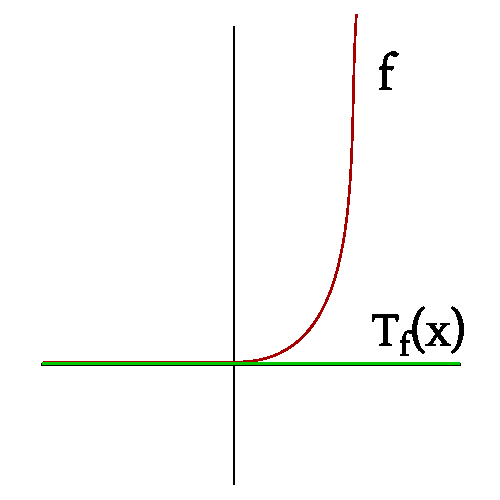
\includegraphics[width=150px]{img/e1x.pdf}
      \caption{Plot of $f$}
      \label{img:e1x}
    \end{center}
  \end{figure}
  \[ f_-^{(n)}(0) = 0 \]
  \[ f_+^{(n)}(0) = \lim_{x\to0^+} f^{(n)}(x) \]

  \[ f^{(n)}(x) = R(x) \cdot e^{-\frac1x} \]
  with $R(x) = \frac{P(x)}{Q(x)}$ with $P$ and $Q$ as polynomials.
  $R$ is a rational function (i.e. division of two polynomials).

  \[ \lim_{x\to0_+} R(x) \cdot e^{-\frac1x} = 0 \]
  Hence $f^{(n)}(0) = 0$ and therefore Taylor series
  $T_f(x; 0) = \sum_{k=0}^\infty \frac{0}{k!} x^k = 0$.
\end{ex}

\begin{rem}
  Taylor:
  \[ R_f(x) = T_f(x; 0) - f(x) \]
  It holds that
  \[ \abs{R_f(x)} \leq c_n \cdot \abs{x}^n \qquad \forall n \in \mathbb N \]
\end{rem}

\begin{theorem}
  Let $f(x) = \sum_{k=0}^\infty a_k (x - x_0)^k$ be a power series in $\xi = x - x_0$.
  Let $\rho(f) > 0$. We already know that $f$ is differentiable for all $\abs{\xi} = \abs{x - x_0} < \rho(f)$ (differentiable by $x$) and $f'$ is a power series with convergence radius $\rho(f') = \rho(f)$.
  \[ f'(x) = \sum_{k=1}^\infty a_k \cdot k x^{k-1} \]
  By complete induction it follows that:
  \begin{itemize}
    \item For all $n \in \mathbb N$ there exists $f^{(n)}(x)$ as power series of form
      \[
        f^{(n)}(x)
        = \sum_{k=n}^\infty a_k \cdot k \cdot (k-1) \cdot (k-2)
          \cdot \ldots (k-n+1) \cdot x^{k-n}
      \]
    \item
      $f^{(n)}$ as convergent power series is a continuous function. Hence,
      \[ f^{(n)}(x_0) = a_n \cdot n \cdot (n-1) \cdot (n-2) \ldots (n-n+1) = a_n \cdot n! \]
      \[ a_n = \frac{f^{(n)}(x_0)}{n!} \]
      Backsubstitution in the power series yields
      \[
        f(x) = \sum_{k=0}^\infty a_k (x - x_0)^k
          = \sum_{k=0}^\infty \frac{f^{(k)}(x_0)}{k!} (x - x_0)^k
          = T_f(x; x_0)
      \]
      Hence $f$ has a power series representation, then the power series is the Taylor series in $f$.
  \end{itemize}
\end{theorem}

\index[English]{Analytical function}
\index[German]{\foreignlanguage{ngerman}{Analytische Funktion}}
\begin{rem}
  A function representable with a power series is called \emph{analytical}.
  In the complex space, once differentiable means arbitrary often differentiable.
\end{rem}

\section{Curves in $\mathbb R^n$}
%
\index[English]{Parametric curve}
\index[German]{\foreignlanguage{ngerman}{Parametrische Kurve}}
\begin{defi}
  A parametric curve is a map $\gamma: I \to \mathbb R^n$ where $I$ is an interval.
  \[
    \gamma(t) = \begin{bmatrix}
      \gamma_1(t) \\
      \gamma_2(t) \\
      \vdots \\
      \gamma_n(t)
    \end{bmatrix}
  \]
  where every function $\gamma_i: I \to \mathbb R$ ($i = 1, \ldots, n$) is continuous.
  Often we write $\gamma_i(t) = x_i(t)$.
  If every $\gamma_i$ is differentiable in $I$, a differentiable, parameterized curve
  is given. $t$ is the curve parameter.

  We call $\Gamma = \setdef{\gamma(t)}{t \in I} = \gamma(I) \subseteq \mathbb R$
  the trace of the curve $\gamma$.
\end{defi}

\begin{ex}
  \[ \gamma: [0, 4\pi] \to \mathbb R^2 \]
  \[ \gamma(t) = \begin{bmatrix} \cos(t) \\ \sin(t) \end{bmatrix} \]
  In this example, every point on the curve is hit twice by the function.

  \[ \Gamma = \setdef{\begin{bmatrix} x_1 \\ x_2 \end{bmatrix} \in \mathbb R}{x_1^2 + x_2^2 - 1 =0 } \]
  $F(x_1, x_2) = x_1^2 + x_2^2 - 1 = 0$ is called trace equation of the curve
  \[ \tilde{\gamma}(t) = \begin{bmatrix} \cos{t} \\ -\sin{t} \end{bmatrix} \text{ in } I = [0, 4\pi] \]

  If $\begin{bmatrix} x_1 \\ x_2 \end{bmatrix} = \begin{bmatrix} \cos{t} \\ \sin{t} \end{bmatrix}$, then
  \[ x_2^1 + x_2^2 - 1 = \cos^2(t) + \sin^2(t) - 1 = 1 - 1 = 0 \]
  On the inverse, let $\begin{bmatrix} x_1 \\ x_2 \end{bmatrix} \in \mathbb R^2$ with $x_1^2 + x_2^2 = 1$. Then there exists $t \in [0,2\pi)$ such that $x_1 = \cos{t}$ and $x_2 = \sin{t}$.

  In this example it holds that $\tilde{\gamma} \neq \gamma$, but $T = \tilde{T}$.
\end{ex}

\begin{ex}
  Let $\tilde{\gamma}(t) = \begin{bmatrix} \cos{t} \\ \sin{t} \end{bmatrix}$.

  \[ \forall \begin{bmatrix} x_1 \\ x_2 \end{bmatrix} \in \tilde{T}: T(x_1, x_2) = x_1^2 + x_2^2 - 1 = 0 \]
  but
  \[ \tilde{T} \neq \setdef{\begin{bmatrix} x_1 \\ x_2 \end{bmatrix}}{F(x_1, x_2) = 0} \]
\end{ex}

\begin{defi}
  Let $\gamma: I \to \mathbb R^n$ be a differentiable, parameterized curve.
  We define
  \[
    \dot{\gamma}(t) =
    \begin{bmatrix} \gamma'_1(t) \\ \gamma'_2(t) \\ \vdots \\ \gamma'_n(t) \end{bmatrix}
    = \begin{bmatrix} x'_1(t) \\ x'_2(t) \\ \vdots \\ x'_n(t) \end{bmatrix}
  \]
  and we call $\dot\gamma(t)$ the derivation vector of $\gamma$ in $t$.
  If $\gamma$ is considered as motion curve, then $\dot\gamma(t)$ is considered as
  speed vector of $\gamma$ in $t$.

  Consider
  \[ \dot{\gamma}(t) = \lim_{h\to 0} \frac{1}{R} \left[\gamma(t + h) - \gamma(t)\right] \]
  as illustrated in Figure~\ref{img:curve_example}.

  \begin{figure}[!h]
    \begin{center}
      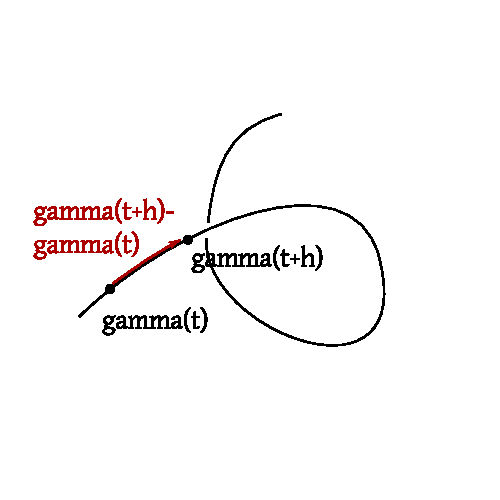
\includegraphics{img/curve_example.pdf}
      \caption{Curve example}
      \label{img:curve_example}
    \end{center}
  \end{figure}

  If $\dot{\gamma}(t) \neq 0$, then $\dot{\gamma}$ is tangential into $\Gamma$
  and we denote $\dot\gamma(t)$ as tangential vector of $\gamma$ in $t$.

  If $\dot\gamma(t) \neq 0$, we set
  \[ T_\gamma(t) = \frac{\dot\gamma(t)}{\norm{\dot\gamma(t)}_2} \]
  and we call $T_\gamma(t)$ the tangential unit vector of $\gamma$ in $t$.
\end{defi}

\begin{ex}
  \[ \gamma: \mathbb R \to \mathbb R^2 \]
  \[ \gamma(t) = \begin{bmatrix} t^2 - 1 \\ t^3 - 1 \end{bmatrix} \text{ differentiable} \]

  \[ \gamma(1) = \begin{bmatrix} 1-1 \\ 1-1 \end{bmatrix} = \vec0 \]
  \[ \gamma(-1) = \begin{bmatrix} 1-1 \\ -1+1 \end{bmatrix} = \vec0 \]

  \begin{figure}[!h]
    \begin{center}
      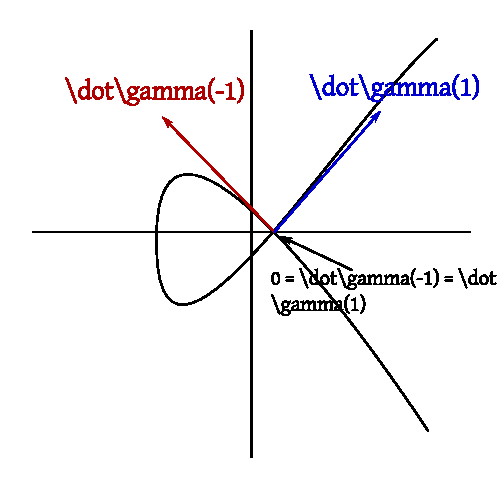
\includegraphics{img/double_point.pdf}
      \caption{A double pointed curve}
      \label{img:dbl-point}
    \end{center}
  \end{figure}

  This curve has a double point, meaning that one point is crossed two times (compare with Figure~\ref{img:dbl-point}).
  \[ \dot\gamma(t) = \begin{bmatrix} 2t \\ 3t^2 - 1 \end{bmatrix} \]
  \[ \dot\gamma(-1) = \begin{bmatrix} -2 \\ 2 \end{bmatrix} \]
  \[ \dot\gamma(1) = \begin{bmatrix} 2 \\ 2 \end{bmatrix} \]
\end{ex}

\index[English]{Regular curve}
\index[German]{\foreignlanguage{ngerman}{Reguläre Kurve}}
\begin{defi}
  % TODO: verify the following notes
  Let $\gamma: I \to \mathbb R^n$ be a differentiable, parameterized curve.
  $\gamma$ is called \emph{regular} curve, if $\dot\gamma(t) \neq \vec0 \forall t \in I$.
\end{defi}

\index[English]{Neil's parabola}
\index[German]{\foreignlanguage{ngerman}{Neilsche Parabel}}
\begin{ex}
  \[ \gamma(t) = \begin{bmatrix} t^2 \\ t^3 \end{bmatrix} \]
  is called \emph{Neil's parabola} and non-regular.
  \[ \dot\gamma(t) = \begin{bmatrix} 2t \\ 3t^3 \end{bmatrix} \]
  \[ \dot\gamma(0) = \vec0 \]
  Has no tangent in the root.
\end{ex}

\begin{figure}[!h]
  \begin{center}
    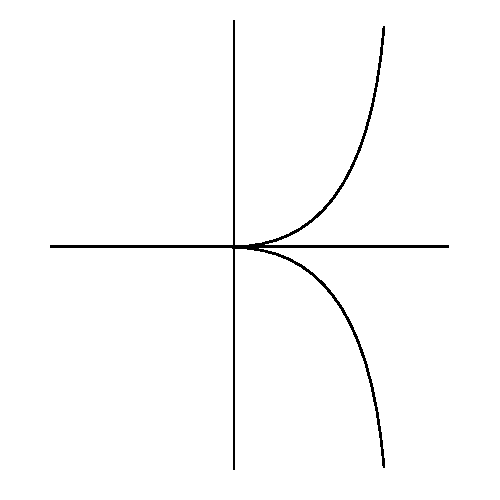
\includegraphics{img/neils_parabola.pdf}
    \caption{Neil's parabola}
  \end{center}
\end{figure}

\begin{ex}
  \[
    \gamma(t)
    = \begin{bmatrix} x_1(t) \\ x_2(t) \end{bmatrix}
    = \begin{bmatrix} a\cos(t) \\ b\sin(t) \end{bmatrix}
  \]
  $a, b > 0$ and $t \in [0,2\pi]$.
  We search for a trace equation of $\gamma$:
  \[
    \frac{x_1(t)}{a} = \cos(t)
    \qquad
    \frac{x_2(t)}{b} = \sin(t)
  \]

  We use the trace equation of the unit circle:
  \[ \left(\frac{x_1}{a}\right)^2 + \left(\frac{x_2}{b}\right)^2 - 1 = 0 \]
  \[ \frac{x_1^2}{a^2} + \frac{x_2^2}{b^2} = 1 \]

  $\gamma$ has an ellipsis as trace with major axes.

  % TODO:
  % TODO: ellipsis.svg
\end{ex}

\meta{lecture}{6th of May 2016}{Wolfgang Ring}

\section{Hyperbolic functions}

\index[English]{Cosine hyperbolic function}
\index[German]{\foreignlanguage{ngerman}{Cosinus Hyperbolicus Funktion}}
\index[English]{Hyperbolic cosine function}
\index[English]{Sine hyperbolic function}
\index[German]{\foreignlanguage{ngerman}{Sine Hyperbolicus Funktion}}
\index[English]{Hyperbolic sine function}
\begin{defi}
  We define the \emph{cosine and sinus hyperbolic functions} as follows:
  \[ \cosh: \mathbb C \to \mathbb C; \cosh(z) = \frac12 \left(e^z + e^{-z}\right) \]
  \[ \sinh: \mathbb C \to \mathbb C; \sinh(z) = \frac12 \left(e^z - e^{-z}\right) \]

  For real values we get Figure~\ref{img:coshsinh}.

  Properties:
  \begin{align*}
    TODO & \\
    \cosh^2(x) - \sinh^2(x) &= \frac14 \left(e^{2x} + 2 e^x + TODO \right) \\
      &= \frac14 \cdot 4 \cdot 1 = 1 \\
    \cosh^2(x) - \sinh(x) &= 1
  \end{align*}
\end{defi}

\begin{figure}[!h]
  \begin{center}
    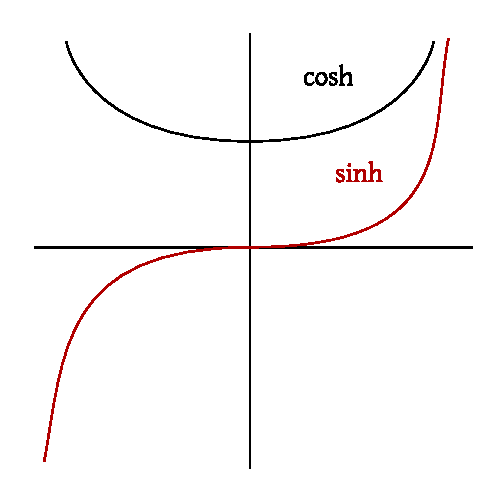
\includegraphics{img/sinhcosh.pdf}
    \caption{Plot of hyperbolic cosine and sine}
    \label{img:coshsinh}
  \end{center}
\end{figure}

\begin{ex}
  Let $y: \mathbb R \to \mathbb R^2$.
  \[
    \gamma(t)
      = \begin{bmatrix} \underbrace{a \cosh(t)}_{>0} \\ b \sinh(t) \end{bmatrix}
      = \begin{bmatrix} x(t) \\ y(t) \end{bmatrix}
  \] \[
    \frac{(x(t))^2}{a^2} - \frac{(y(t))^2}{b^2} = \cosh^2(t) - \sinh^2(t) = 1
  \]
  hence the trace $T$ of $\gamma$ is inside the hyperbola
  \[ H = \setdef{\begin{bmatrix} x \\ y \end{bmatrix} \in \mathbb R^2}{\frac{x^2}{a^2} - \frac{y^2}{b^2} = 1} \]
  \begin{figure}[h!]
    \begin{center}
      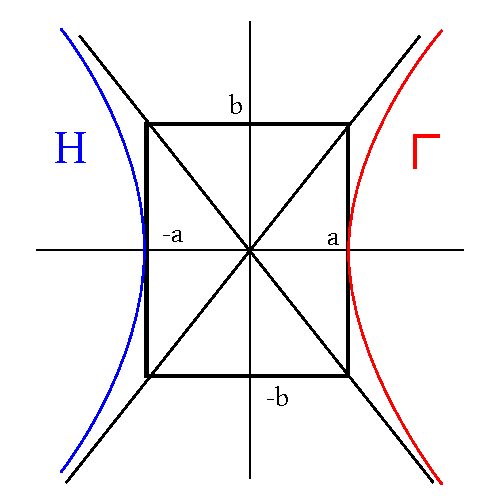
\includegraphics{img/hyperbolic_hyperbola.pdf}
      \caption{Hyperbola $H$}
    \end{center}
  \end{figure}
\end{ex}

\begin{theorem}
  Let $I \subseteq \mathbb R$ be an interval and $f: I \to \mathbb R$
  continuously differentiable. Then
  \[
    \left.\begin{array}{c}
      t \mapsto \begin{bmatrix} t \\ f(t) \end{bmatrix} \\
      I \to \mathbb R^2
    \end{array}\right\}
  \]
  a parametric, differentiable curve.
  The function graph is equivalent to the trace of the curve.
\end{theorem}

\begin{theorem}[Representation as function graph]
  Let $\gamma: I \to \mathbb R^2$ a continuously differentiable curve,
  $I$ is an interval and
  \[
    \gamma(t) = \begin{bmatrix} \gamma_1(t) \\ \gamma_2(t) \end{bmatrix}
    = \begin{bmatrix} x(t) \\ y(t) \end{bmatrix}
  \]
  it holds that
  \[ \dot{\gamma}_1(t) \neq 0 \quad \forall t \in I \]
  Then there exists a continuously differentiable function
  $f: J = \gamma_1(I) \to \mathbb R$ such that the graph of $f$
  matches the trace of $\gamma$.

  Let $x_0 = \gamma_1(t_0)$. Then it holds that
  \[ f'(x_0) = \frac{\dot{y}(t_0)}{\dot{x}(t_0)}. \]
  If $\gamma$ is differentiable twice in $t_0$,
  then $f$ is differentiable twice in $x_0$.
  \[ f''(x_0) = \frac{\dot{x}(t_0) \ddot{y}(t_0) - \ddot{x}(t_0) \dot{y}(t_0)}{[\dot{x}(t_0)]^3} \]
\end{theorem}
\begin{proof}
  $\dot{y}_1$ has no root, is continuous,
  this means $\dot{\gamma}_1$ has a uniform sign in $I$.
  Hence $\gamma_1$ is strictly monotonical in $I$.
  So $\gamma_1: I \to J = \gamma_1(I)$ is bijective.

  Let $\gamma_1^{-1}: J \to I$ be the inverse function.
  Because $\dot{\gamma}_1 \neq 0$ in $I$ is $\gamma_1^{-1}$ is differentiable
  with
  \[ \left(\gamma_1^{-1}\right)'(s) = \frac{1}{\dot{\gamma}_1(\gamma_1^{-1}(s))} \]
  We define \[ f(x) = \gamma_2(\gamma_1^{-1}(x)) \]
  \[ I \to \mathbb R \]

  Let $T_f = \setdef{(x, f(x))}{x \in I}$ be the graph of $f$ and $(x, f(x)) \in T_f$;
  $(x, f(x)) = (x, \gamma_2(\gamma_1^{-1}(x)))$.
  Let $\gamma_1^{-1}(x) = t \in I$ and therefore $x = \gamma_1(t)$. So it holds that
  \[ (x, f(x)) = (\gamma_1(t), \gamma_2(t)) \in T \qquad \text{\dots{} trace of } \gamma \]

  On the opposite, we have $(\gamma_1(t), \gamma_2(t)) \in T$.
  Let $x = \gamma_1(t) \in J$ and $t = \gamma_1^{-1}(x)$ and $(\gamma_1(t), \gamma_2(t)) = (x, \gamma_2(\gamma_1^{-1}(x))) = (x, f(x)) \in T_f$.

  \[ \left.f'(x)\right|_{x = x_0} = \dot{\gamma}_2(\gamma_1^{-1}(x_0)) \cdot \frac{1}{\dot{\gamma}_1^{-1}(x_0)} = \frac{\dot{y}(t_0)}{\dot{x}(t_0)} \]
  Let $\gamma_1^{-1}(x_0) = t_0$.

  \[
    f''(x_0) = \frac{\ddot{\gamma_2}(t_0) \cdot \frac{1}{\dot{\gamma}_1(t_0)} \cdot \dot{\gamma}_1(t_0) - \dot{\gamma}_2(t_0) \cdot \ddot{\gamma}_1(t_0) \cdot \frac{1}{\dot{\gamma}_1(t_0)}}{(\dot{\gamma}_1(t_0))^2}
  \] \[
    = \frac{\ddot{\gamma}_2(t_0) \cdot \dot{\gamma}_1(t_0) - \ddot{\gamma}_1(t_0) \cdot \dot{\gamma}_2(t_0)}{(\dot{x}(t_0))^3}
  \]
  \[ = \frac{\ddot{\gamma}(t_0) \cdot \dot{x}(t_0) - \dot{y}(t_0) \ddot{x}(t_0)}{(\dot{x}(t_0))^3} \]
\end{proof}

TODO

\begin{figure}[h!]
  \begin{center}
    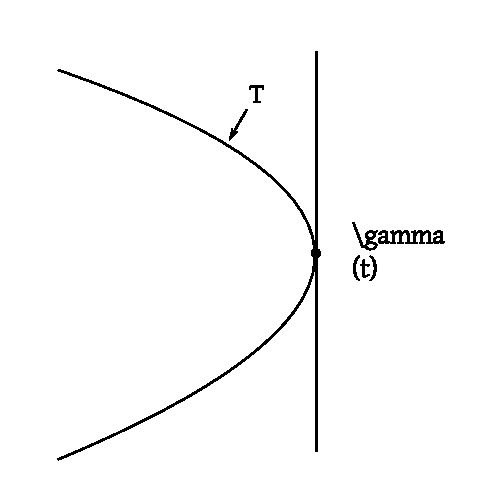
\includegraphics{img/parametric_curve_hyperbola.pdf}
    \caption{Parametric curve}
  \end{center}
\end{figure}

\section{Arc length of a parametric curve}
%
\begin{theorem}
  Let $\gamma: I = [a,b] \to \mathbb R^n$ be a parametric curve.
  Let $z = \set{t_0 = a, t_1, t_2, \ldots, t_N = b}$ with $t_{i-1} < t_i$
  for $i = 1, \ldots, N$ be a partition of the interval $I$.
  We denote the length of the polygonal line through the partition points
  $\gamma(t_0)$, $\gamma(t_1)$, \ldots, $\gamma(t_N)$ with
  \[ s(z) = s_{\gamma}(z) = \sum_{i=1}^{N} \norm{\gamma(t_1) - \gamma(t_{i-1})} \]

  Let $z^*$ be more detailed than $z$. Then it holds that
  \[ s(z^*) \geq s(z) \]
\end{theorem}
\begin{figure}[!h]
  \begin{center}
    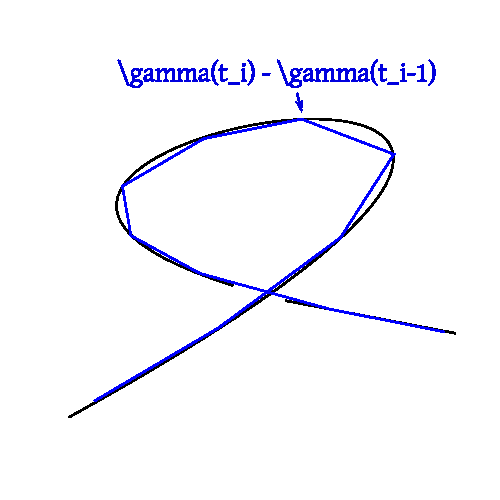
\includegraphics{img/arc.pdf}
    \caption{Approximation of the arc length}
  \end{center}
\end{figure}
\begin{proof}[Insertion of partition points]
  Let $z = \set{t_0 < t_1 < \ldots < t_N}$ and $z^* = \set{t_0 < \ldots < t_{k-1} < t' < t_k < \ldots < t_N}$.
  \begin{align*}
    s(z)   &= \sum_{i=1}^N \norm{\gamma(t_i) - \gamma(t_{i-1})} \\
    s(z^*) &= \sum_{i=1}^{k-1} \norm{\gamma(t_i) - \gamma(t_{i-1})} \\
           & + \underbrace{\norm{\gamma(t') - \gamma(t_{k-1})} + \norm{\gamma(t_k) - \gamma(t')}}_{\geq \norm{\gamma(t_K) - \gamma(t') + \gamma(t') - \gamma(t_{K-1})}} \\
           &+ \sum_{i=K+1}^N \norm{\gamma(t_i) - \gamma(t_{i-1})} \\
           &\geq \sum_{i=1}^N \norm{\gamma(t_1) - \gamma(t_{i-1})} = s(z)
  \end{align*}
  For insertion of multiple points use induction.
\end{proof}

\index[English]{Rectifiable curve}
\index[German]{\foreignlanguage{ngerman}{Rektifizierbare Kurve}}
\index[English]{Length of a curve}
\index[German]{\foreignlanguage{ngerman}{Länge einer Kurve}}
\index[English]{Curve length}
\index[German]{\foreignlanguage{ngerman}{Kurvenlänge}}
\begin{defi}
  Let $\gamma: I = [a,b] \to \mathbb R^n$ be a continuous curve.
  $\gamma$ is call \emph{rectifiable} if
  \[ s(\gamma) = \sup{s(z)} < \infty \]
  where $z$ is a partition of $I$.
  In this case $s(\gamma)$ is called length of curve $\gamma$.
\end{defi}
\begin{ex}
  Let $\gamma: I \to \mathbb R^n$ be Lipschitz continuous.
  Hence
  \[ \exists L \geq 0: \norm{\gamma(s) - \gamma(t)} \leq L(s - 1)  \]
  for all $s,t \in I$. Then $\gamma$ is rectifiable and $s(\gamma) \leq L \cdot (b-a)$.
\end{ex}
\begin{proof}
  Let $z$ be a partition of $I$.
  \[ z = \set{t_0 < t_1 < t_2 < \ldots < z_N} \]
  Then it holds that
  \begin{align*}
    s(z) &= \sum_{i=1}^N \norm{\gamma(t_i) - \gamma(t_{i-1})} \\
         &\leq \sum_{i=1}^N L \abs{t_i - t_{i-1}} \\
         &= L \sum_{i=1}^N (t_i - t_{i-1}) \\
         &= L (t_N - t_0) = L(b - a)
  \end{align*}
\end{proof}

\begin{theorem}
  Let $\gamma: I \to \mathbb R^n$ be a continuous curve.
  \[
    \gamma(t) = \begin{bmatrix}
      \gamma_1(t) \\
      \vdots \\
      \gamma_n(t)
    \end{bmatrix}
  \]
  Let every $\gamma_i: I \to \mathbb R$ be a primitive function of a regulated function
  (hence $\dot{\gamma}_i$ exists for all $t$ except for finitely many points,
  furthermore $\dot{\gamma}_i$ has left-sided and right-sided limits everywhere).
  \[ I = [a,b] \]
  Then $\gamma$ is rectifiable and it holds that
  \[ s(\gamma) = \int_a^b \norm{\dot{\gamma}(t)} \, dt \]
\end{theorem}

\begin{rem}[Some necessary preparations]
  \[
    \int_a^b \gamma(t) \, dt \coloneqq
    \begin{bmatrix}
      \int_a^b \gamma_1(t) \, dt \\
      \int_a^b \gamma_2(t) \, dt \\
      \vdots \\
      \int_a^b \gamma_n(t) \, dt
    \end{bmatrix}
  \]
\end{rem}

\begin{lemma}
  Let $\gamma: [a,b] \to \mathbb R^n$ be a continuous curve.
  Then it holds that
  \[ \norm{\int_a^b \gamma(t) \, dt} \leq \int_a^b \norm{\gamma(t)} \, dt \]
\end{lemma}
\begin{proof}
  Let $\varphi_i$ be a step function which approximates $\gamma_i$ uniformly.
  Hence, we assume that $\inorm{\varphi_i - \gamma_i} < \varepsilon$.
  $z_i$ is a partition such that $\varphi_i$ is constant at every interval.

  Define $z = \bigcup_{i=1}^n z_i$ ascendingly ordered.
  Then every $\varphi_i$ is also a step function in terms of $z$.
  \[ z = \set{t_0 < t_1 < \ldots < t_N} \]
  \[ \varphi_i(t) = c^i_k \quad \text{ for } t \in (t_{k-1}, t_k) \]
  \[ \int_a^b \varphi_i(t) \, dt = \sum_{k=1}^n c_k^i (t_k - t_{k-1}) \]
  Build
  \[
    \varphi(t) = \begin{bmatrix}
      \varphi_1(t) \\
      \vdots \\
      \varphi_N(t)
    \end{bmatrix}
  \]
  Then it holds that
  \[
    \norm{\int_a^b \varphi(t) \, dt} = \norm{
      \begin{bmatrix}
        \sum_{k=1}^N c_k^1 (t_k - t_{k-1}) \\
        \sum_{k=1}^N c_k^2 (t_k - t_{k-1}) \\
        \vdots \\
        \sum_{k=1}^N c_k^n (t_k - t_{k-1})
      \end{bmatrix}
    } = \norm{\sum_{k=1}^N (t_k - t_{k-1}) \cdot \begin{bmatrix} c_k^1 \\ \vdots \\ c_k^n \end{bmatrix}}
  \] \[
    \underbrace{\leq}_{\text{triangle ineq. in } \mathbb R^n} \sum_{k=1}^N (t_k - t_{k-1})
    \norm{\begin{bmatrix} c_k^1 \\ \vdots \\ c_k^n \end{bmatrix}}
    = \int_a^b \underbrace{\norm{\varphi(t)}}_{\text{step function in } \mathbb R} \, dt
  \] \[
    \norm{\gamma(t) - \varphi(t)} = \left(\sum_{i=1}^n \abs{\gamma_i(t) - \varphi_i(t)}^2\right)^{\frac12}
  \] \[
    \leq \left(\sum_{i=1}^n \varepsilon^2\right)^{\frac12} = \sqrt{n} \cdot \varepsilon
  \] \[
    \Rightarrow \int_a^b \norm{\gamma(t) - \varphi(t)} \, dt < \varepsilon \sqrt{n} (b - a)
   \] \[
    \norm{\int_a^b (\gamma(t) - \varphi(t)) \, dt} = \norm{
      \begin{bmatrix}
        \int_a^b \gamma_1(t) - \varphi_1(t) \, dt \\
        \int_a^b \gamma_2(t) - \varphi_2(t) \, dt \\
        \vdots \\
        \int_a^b (\gamma_n(t) - \varphi_n(t)) \, dt
      \end{bmatrix}
    }
  \] \[
    = \norm{\begin{bmatrix}
      \abs{\int_a^b (\gamma_1(t) - \varphi_1(t)) \, dt} \\
      \abs{\int_a^b (\gamma_2(t) - \varphi_2(t)) \, dt} \\
      \vdots \\
      \abs{\int_a^b (\gamma_n(t) - \varphi_n(t)) \, dt}
    \end{bmatrix}}
    \leq
    \norm{\begin{bmatrix}
      \varepsilon (b - a) \\
      \varepsilon (b - a) \\
      \vdots \\
      \varepsilon (b - a) \\
    \end{bmatrix}}
    = \varepsilon (b - a) \sqrt{n}
  \]
  Hence it holds that
  \[
    \norm{\int_a^b \gamma(t) \, dt}
    = \norm{\int_a^b \varphi(t) \, dt - \int_a^b (\varphi(t) - \gamma(t)) \, dt}
  \] \[
    \leq \norm{\int_a^b \varphi(t) \, dt} + \norm{\int_a^b (\varphi(t) - \gamma(t)) \, dt}
  \] \[
    \leq \int_a^b \norm{\varphi(t)} \, dt + \varepsilon (b - a) \sqrt{n}
  \] \[
    \leq \int_a^b \left(\norm{\varphi(t) - \gamma(t)} + \norm{\gamma(t)}\right) \, dt
    + \varepsilon (b - a) \sqrt{n}
  \] \[
    \leq \varepsilon (b - a) \sqrt{n} + \int_a^b \norm{\gamma(t)} \, dt + \varepsilon (b - a) \sqrt{n}
  \]
  Hence
  \[ \norm{\int_a^b \gamma(t) \, dt} \leq \int_a^b \norm{\gamma(t)} \, dt + 2 \varepsilon (b - a) \sqrt{n} \qquad \forall \varepsilon > 0 \]
  Hence
  \[ \norm{\int_a^b \gamma(t) \, dt} \leq \int_a^b \norm{\gamma(t)} \, dt \]
\end{proof}

\meta{lecture}{10th of May 2016}{Wolfgang Ring}

\begin{proof}[Proof of the formula for the arc length]
  Its definition depends on the parameterization.
  \[ s(\gamma) = \sup_z{s(z)} \]
  \[ s(z) = \sum_{k=1}^N \norm{\gamma(t_k) - \gamma(t_{k-1})} \]

  We show:
  \begin{enumerate}
    \item
      For all decompositions of $z$, it holds that
      \[ s(z) \leq \int_a^b \norm{\dot\gamma(t)} \, dt \]
      \[ \Rightarrow s(\gamma) \leq \int_a^b \norm{\dot\gamma(t)} \, dt \]
    \item
      \[ \forall \varepsilon > 0 \exists \text{ decomposition } z: s(\gamma) \geq s(z) \geq \int_a^b \norm{\dot\gamma(t)} \, dt - \varepsilon \]
  \end{enumerate}

  \begin{enumerate}
    \item Let $z = \set{t_0 < t_1 < \ldots < t_N}$.
      \begin{align*}
        s(z) &= \sum_{k=1}^N \norm{\gamma(t_k) - \gamma(t_{k-1})}  \\
          &\overset{\substack{\text{fundamental} \\ \text{theorem}}}{=}
            \sum_{k=1}^N \norm{\int_{t_{k-1}}^{t_k} \dot\gamma(t) \, dt} \\
          &\overset{\text{Lemma}}{=}
            \sum_{n=1}^n \int_{t_{k-1}}^{t_k} \norm{\dot\gamma(t)} \, dt \\
          &\sum_{n=1}^N TODO
      \end{align*}
    \item Let $\varepsilon > 0$ be arbitrary.
      Find decomposition $z$ such that $s(\gamma) \geq s(z) \geq \int_a^b \norm{\dot\gamma(t)} \, dt - \varepsilon$.
      Let
      \[ \varphi(t) = \begin{bmatrix} \varphi_1(t) \\ \vdots \\ \varphi_n(t) \end{bmatrix} \]
      and $\varphi_t$ is a step function in $[a,b]$.

      Every $\varphi_i$ is constant in ($t_{k-1}, t_k$) for $k=1,\ldots,N$.
      and we let $z = \set{t_0, t_1, \ldots, t_N}$.
      Let $\varphi_i$ such that $\inorm{\dot\gamma_i - \varphi_i} \leq \frac{\varepsilon}{2(b - a) \sqrt{N}}$.

      Then it holds that $\forall t \in [a,b]$:
      \[ \norm{\dot\gamma(t) - \gamma(t)} = \left(\sum_{i=1}^n \abs{\dot\gamma_i(t) - \varphi_i(t)}\right)^{\frac12} \]
      \[
        \leq \left(\sum_{i=1}^n \inorm{\dot\gamma_i - \varphi_i}^2\right)^{\frac12}
        \leq \left(\sum_{i=1}^n \left(\frac{\varepsilon}{2(b - a)}^2 \cdot \frac1n\right)\right)^[\frac12]
        = \frac{\varepsilon}{2 (b - a)}
      \]
      We let
      \begin{align*}
        \inorm{\dot\gamma - \varphi}
          &= \sup\set{\norm{\dot\gamma(t) - \varphi(t)}_2: t \in [a,b]} \\
          &= \max\set{\norm{\dot\gamma(t) - \varphi(t)}_2: t \in [a,b]}
      \end{align*}
      It holds that
      \[ \inorm{\dot\gamma - \varphi} < \frac{\varepsilon}{2 (b - a)} \]
      \[ z = \set{t_0, t_1, \ldots, t_N} \]
      \[
        \norm{\int_{t_{k-1}}^{t_k} \dot\gamma(t) \, dt}
        = \norm{\int_{t_{k-1}}^{t_k} (\dot\gamma(t) - \varphi(t)) \, dt + \int_{t_{k-1}}^{t_k} \varphi(t) \, dt}
      \] \[
        \geq \norm{\int_{t_{k-1}}^{t_k} \varphi(t) \, dt} - \norm{\int_{t_{k-1}}^{t_k} (\dot\gamma(t) - \varphi(t)) \, dt}
      \]
      $\varphi$ is constant and the right summand is $\leq \int_{t_{k-1}}^{t_k} \norm{\dot\gamma(t) - \varphi(t)} \, dt$.
      \[
        \geq \int_{t_{k-1}}^{t_k} \norm{\varphi(t)} \, dt - \int_{t_{k-1}}^{t_k} \underbrace{\norm{\dot\gamma(t) - \varphi(t)}}_{< \frac{\varepsilon}{2(b-1)}} \, dt
      \] \[
        > \int_{t_{k-1}}^{t_k} \norm{\varphi(t)} \, dt - \frac{\varepsilon}{2(b - a)} (t_k - t_{k-1})
      \] \[
        s(z) = \sum_{k=1}^N \norm{\int_{t_{k-1}}^{t_k} \dot\gamma(t) \, dt}
          > \sum_{k=1}^N \int_{t_{k-1}}^{t_k} \norm{\varphi(t)} - \frac{\varepsilon}{2(b - a)} (t_{k} - t_{k-1})
      \] \[
        = \int_a^b \norm{\varphi(t)} \, dt - \frac{\varepsilon}{2(b - a)} \underbrace{(t_N - t_0)}_{= b - a}
      \] \[
        = \int_a^b \norm{\varphi(t)} \, dt - \frac{\varepsilon}{2}
      \]

      \[
        \int_a^b \norm{\varphi(t)} \, dt = \int_a^b \norm{\varphi(t) - \dot\gamma(t) + \dot\gamma(t)} \, dt
      \] \[
        \geq \int_a^b \left(\norm{\dot\gamma(t)} - \underbrace{\norm{\varphi(t) - \dot\gamma(t)}}_{< \frac{\varepsilon}{2(b - a)}}\right) \, dt
      \] \[
        = \int_a^b \norm{\dot\gamma(t)} \, dt - \frac{\varepsilon}{2}
      \] \[
        \Rightarrow s(z) > \int_a^b \norm{\dot\gamma(t)} \, dt - \frac\varepsilon2 - \frac\varepsilon2
      \] \[
        \Rightarrow s(\gamma) \geq s(z) > \int_a^b \norm{\dot\gamma(t)} \, dt - \varepsilon
        \qquad \forall \varepsilon > 0
      \] \[
        \Rightarrow s(\gamma) \geq \int_a^b \norm{\dot\gamma(t)} \, dt
      \]
  \end{enumerate}
\end{proof}

\begin{ex}[Circumference of a circle with radius $r$]
  \[
    \gamma_r(t) = r \begin{bmatrix}
      \cos(t) \\
      \sin(t)
    \end{bmatrix}
    \qquad t \in [0, 2\pi];
    \dot\gamma_t(t) = r \begin{bmatrix}
      -\sin(t) \\
      \cos(t)
    \end{bmatrix}
  \] \[
    s(\gamma_r) = \int_0^{2\pi} \norm{r \begin{bmatrix} - \sin(t) \\ \cos(t) \end{bmatrix}} \, dt
    = \int_0^{2\pi} r \, dt = 2\pi r
  \]
\end{ex}

\index[English]{Elliptic integral}
\index[German]{\foreignlanguage{ngerman}{Elliptisches Integral}}
\begin{ex}[Ellipsis]
  \[
    \gamma(t) = \begin{bmatrix}
      a \cos(t) \\
      b \sin(t)
    \end{bmatrix} \qquad a,b > 0
  \] \[
    \dot\gamma(t) = \begin{bmatrix}
      -a \sin(t) \\
      b \cos(t)
    \end{bmatrix}
  \] \[
    \norm{\dot\gamma(t)} = (a^2 \underbrace{\sin^2(t)}_{1 - \cos^2(t)} + b^2 \cos^2 (t))^{\frac12}
  \]
  Let $a \geq b$, $\varepsilon^2 = 1 - \frac{b^2}{a^2}$.
  \begin{align*}
    \norm{\dot\gamma(t)} &= (a^2 - (a^2 - b^2) \cos^2(t))^{\frac12} \\
      &= a \left(1 - \left(1 - \frac{b^2}{a^2}\right) \cos^2(t)\right)^2 \\
      &= a \left(1 - \varepsilon^2 \cos^2(t)\right)^{\frac12}
  \end{align*}
  \[ s(\gamma) = a \int_0^{2\pi} \sqrt{1 - \varepsilon^2 \cos^2(t)} \, dt \]
  This defines a new set of functions which cannot be solved with means we discussed so far.
  They are called \emph{elliptic integral}.
\end{ex}

\subsection{Change of parameters, reparameterization}
\index[English]{Reparameterization}
\index[German]{\foreignlanguage{ngerman}{Reparametrisierung}}
%
Let $\sigma: I \to J$ as smooth (ie. differentiable) as required.
$\sigma$ is bijective and $\sigma^{-1}: J \to I$ is be part
of the same differentiation class like $\sigma$.
Let $\gamma: I \to \mathbb R^n$ be a curve. We call
$\beta = \gamma \circ \sigma^{-1}: I \to \mathbb R^n$ a reparameterization
of $\gamma$ using $\sigma$. Compare with Figure~\ref{img:reparam}.

\begin{figure}[!h]
  \begin{center}
    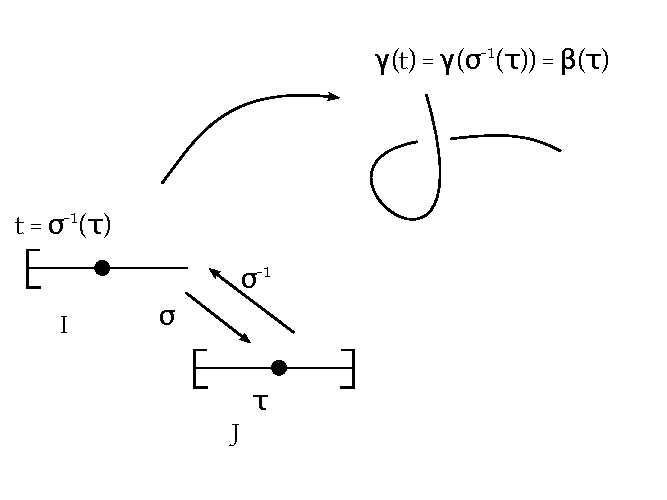
\includegraphics{img/reparameterization.pdf}
    \caption{Reparameterization: $\beta$ and $\gamma$ have the same trace}
    \label{img:reparam}
  \end{center}
\end{figure}

\index[English]{Orientation preserving reparameterization}
\index[German]{\foreignlanguage{ngerman}{Orientierungserhaltende Reparameterisierung}}
$\sigma$ is called parameter transformation.
$\gamma$ is called orientation preserving, if $\sigma$ is strictly monotonically
decreasing.

\index[English]{Geometric curve measures}
\index[German]{\foreignlanguage{ngerman}{Geometrisches Maß}}
A measure, defined by the curve (arc length, tangential vector, curvature, \dots)
is called \emph{geometric}, if reparameterization can be applied without modifications.

$s(\gamma)$ is obviously a geometric measure, because
\begin{enumerate}
  \item By definition of polygonal lines
  \item Let $\beta(\tau) = \gamma \circ \sigma^{-1}(\tau)$.
    \[ \dot{\beta}(\tau) = \dot{\gamma}(\sigma^{-1}(\tau)) \circ (\sigma^{-1})'(\tau) \]
    \[ \norm{\dot\beta(\tau)} = \norm{\dot\gamma(\sigma^{-1})(\tau)} \cdot \abs{(\sigma^{-1})'(\tau)} \]
    \begin{description}
      \item[Case $\sigma$ is orientation preserving]
        If and only if $\sigma' > 0 \Leftrightarrow (\sigma^{-1})' > 0$

        Let $I = [a,b]; J = [c,d]; c = \sigma(a); d = \sigma(b)$.
        \[ s(\beta) = \int_c^d \norm{\dot\gamma(\underbrace{\sigma^{-1}(\tau)}_{= t})} \cdot \underbrace{(\sigma^{-1})' (\tau) \, d\tau}_{dt} \]
        \[ = \int_a^b \norm{\dot\gamma(t)} \, dt = s(\gamma) \qquad \text{ (by substitution)} \]
      \item[Case $\sigma$ is orientation inversing]
        \[ \gamma' < 0 \qquad (\gamma^{-1})' < 0 \]
        \[ \abs{(\sigma^{-1})'(\tau)} = -(\sigma^{-1})'(\tau) \qquad \sigma(a) = d, \sigma(b) = c \]
        \[
          \int_c^d \norm{\dot\beta(\tau)} \, d\tau
          = \int_c^d \norm{\dot\gamma(\underbrace{\sigma^{-1}(\tau)}_{t})} \cdot \underbrace{\left(- (\sigma^{-1})'(\tau)\right)\, d\tau}_{dt}
        \] \[
          \begin{vmatrix}
            \tau = c \Leftrightarrow t = b \\
            \tau = a \Leftrightarrow t=  a
          \end{vmatrix}
        \] \[
          = -\int_b^a \norm{\dot\gamma(t)} \, dt
        \] \[
          = \int_a^b \norm{\dot\gamma(t)} \, dt = s(\gamma)
        \]
    \end{description}
\end{enumerate}

\subsection{Reparameterization by arc length}
%
We consider a regular curve $\gamma$, hence $\norm{\dot\gamma(t)} > 0 \quad \forall t \in I$
and let $s: I \to J = S(I)$ by
\[ s(t) = \int_a^t \norm{\dot\gamma(\tau)} \, d\tau \]

$s(t)$ is the length of the curve $\gamma$ between $a$ and $t$. Let $s(a) = 0$.
It holds that $\dot{s}(t) = \norm{\dot\gamma(t)} > 0$ (by the Fundamental Theorem of Differential and Integration Theory), hence $s$ is strictily monotonically increasing.
We use $s$ for reparameterization.
\[ \beta(\xi) = \gamma \circ s^{-1}(\xi) \]
is a reparameterization of $\gamma$ by the arc length.

\begin{align*}
  \norm{\dot\beta(\xi)}
    &= \norm{\dot\gamma(s^{-1}(\xi)) \circ (s^{-1})'(\xi)} \\
    &= \norm{\dot\gamma(s^{-1}(\xi)) \frac{1}{\dot{s}(s^{-1}(\xi))}} \\
    &= \norm{\dot\gamma(s^{-1})(\xi)} \cdot \abs{\frac{1}{\dot{s} (s^{-1}(\xi))}} \\
    &= \frac{\norm{\dot{\gamma}(s^{-1}(\xi))}}{\norm{\dot\gamma(s^{-1}(\xi))}} = 1
\end{align*}
Hence the tangential vector is the unit vector (in every point)
\[ s_{\beta}(\xi) = \int_0^{\xi} \underbrace{\norm{\dot\beta(\eta)}}_{=1} \, d\eta = \xi \]
So the curve parameter corresponds to the arc length.
On the opposite: Let $\gamma: I \to \mathbb R^n$ with property $\norm{\dot\gamma(t)} = 1 \quad\forall t \in I = [0,b]$.
Then it holds that
\[ s(t) = \int_0^t \underbrace{\norm{\dot\gamma(\tau)}}_{=1} \, d\tau = t \]
So it holds that $s = s^{-1} = \operatorname{id}_{[0,b]}$.
So $\gamma$ is parameterized by the arc length.

\begin{rem}[Notation]
  We don't write $\xi = s(t)$, but $s = s(t)$.
\end{rem}

Reparameterization by the arc length:
\[ \beta(s) = \gamma(s^{-1}(s)) = \gamma(t) \]

\meta{lecture}{12th of May 2016}{Wolfgang Ring}

\subsection{Invariance of arc length}
%
Let $\gamma: I \to \mathbb R$ be a parameterized curve.
\[ \sigma: I \to J \text{ orientation-preserving parameter transformation} \]
\[ S_\gamma(t) = \int_a^t \norm{\dot\gamma(\xi)} \, d\xi \]
\[ I = [a,b] \qquad J = [c,d] \]

\[ \tilde{\gamma} = \gamma \circ \sigma^{-1}: J \to \mathbb R^n \quad \text{ reparameterization} \]
\[ S_{\tilde{\gamma}}(\tau) = \int_C^\tau \abs{\dot{\tilde{\gamma}}(\eta)} \, d\eta \]
We know that $S_{\tilde{\gamma}}(\tau) = S_{\tilde{\gamma}}(\sigma(t)) = S_{\gamma}(t)$.
\[ S_{\tilde{\gamma}} \circ \sigma = S_{\gamma} \]
Let $S = S_{\gamma}(t)$ and $\beta$ is a reparameterization of $\gamma$ by its arc length.
Hence $\beta(s) = \gamma(s^{-1}_\gamma(s))$ and $\beta = \gamma \circ S_{\gamma}^{-1}$.

\[ \tilde{\beta}(s) = \tilde{\gamma} \circ S_{\tilde{\gamma}}^{-1} = \gamma \circ \sigma^{-1} \circ \sigma \circ S_{\gamma}^{-1} = \gamma \circ S_{\gamma}^{-1} = \beta(s) \]

Hence, reparameterized curves $\gamma$ and $\tilde{\gamma}$ have the same reparameterization by its arc length $\beta$.

We require orientation preservation (compare with Figure~\ref{img:arclength}).
%
\begin{figure}[!h]
  \begin{center}
    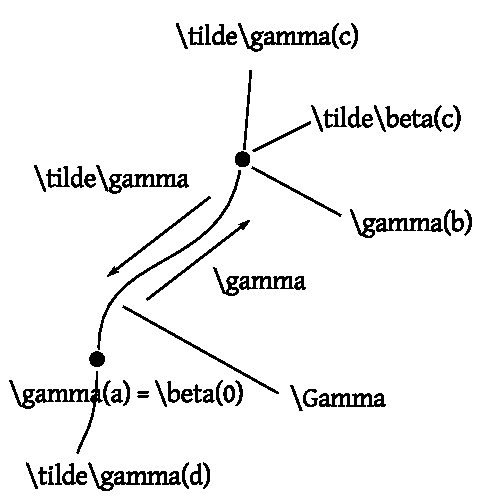
\includegraphics{img/arc_length_invariance.pdf}
    \caption{Invariance of arc length}
    \label{img:arclength}
  \end{center}
\end{figure}

Then it holds that
\[ \tilde{\beta}(s) = \beta(s(\gamma) - s) \]

Consider special case $\gamma: I \to \mathbb R^2$.

\[
  \gamma(t) = \begin{bmatrix} x(t) \\ y(t) \end{bmatrix};
  \qquad
  S_\gamma(t) = \int_a^t \sqrt{\dot{x}(\xi)^2 + \dot{y}(\xi)^2} \, d\xi
\]
or even more special:
\[ \gamma(t) = \begin{bmatrix} t \\ f(t) \end{bmatrix} \qquad \text{ \dots function graph} \]
\[ S_\gamma(t) = S_f(t) = \int_a^t \sqrt{1 + (f'(\xi))^2} \, d\xi \]


\subsection{Curvature}
%
Curvature corresponds to the rate of change of the direction of motion.
This corresponds to the rate of change of
\[ T(t) = \frac{\dot{\gamma}(t)}{\abs{\gamma(t)}} \]
in regards of the arc length.

\begin{enumerate}
  \item Let $\gamma: I \to \mathbb R^2$ be a parameterized regular curve.
    $\beta(s)$ is the reparameterization of $\gamma$ by its arc length.
    $\beta: [0, s(\gamma)] \to \mathbb R^2$.
    \[ \dot\beta(s) = T(s) \quad \text{ is a unit vector} \]
    It holds that $\langle \dot\beta(s), \dot\beta(s)\rangle = 1$,
    hence $\dot\beta_1^2(s) + \dot\beta_2^2(s) = 1$.
    $\beta$ can be differentiated twice.

    So we derive $\dot\beta_1^2(s) + \dot\beta_2^2(s)$:
    \[ 2\dot\beta_1(s) \cdot \ddot{\beta_1}(s) + 2 \dot\beta_2(s) \cdot \ddot{\beta}_2(s) = 0 \]
    So it holds with
    \[
      \ddot{\beta}(s) = \begin{bmatrix} \ddot{\beta}_1(s) \\ \ddot{\beta}_2(s) \end{bmatrix}
      \qquad
      \langle \dot{\beta}(s), \ddot{\beta}(s) \rangle = 0
    \]
    $\ddot{\beta}$ is orthogonal to $\dot{\beta} = T$.
    We define $N = \begin{bmatrix} -\dot{\beta}_2 \\ \dot{\beta}_1 \end{bmatrix} = \begin{bmatrix} 0 & -1 \\ 1 & 0 \end{bmatrix} \cdot T$.
\end{enumerate}

\begin{defi}
  We define a \emph{signed} curvature $\kappa$ in $\gamma$ in point $\gamma(t) = \beta(s)$
  by its relation
  \[ \frac{d^2 \beta}{ds^2} = \ddot{\beta}(s) = \kappa(S) \cdot N(S) \]
  $\kappa$ (with this property) actually exists, because $\ddot{\beta}$ is orthogonal to $T$
  and therefore a multiple of $N$.

  In case of reparameterization $\gamma(t) = \tilde{\gamma}(\tau)$, the arc length stays
  the same. Therefore the curvature in $\gamma(t)$ and $\dot{\gamma}(\tau)$ is also the same.
  Hence the curvature is invariant in terms of orientation-preserving reparameterization.
\end{defi}

\meta{lecture}{13th of May 2016}{Wolfgang Ring}




%\index[English]{}
%\index[German]{\foreignlanguage{ngerman}{}}

\clearpage
\begin{otherlanguage}{ngerman}
\printindex[German]
\end{otherlanguage}
\printindex[English]

\end{document}

%%% Local Variables:
%%% mode: latex
%%% TeX-master: t
%%% End:
